\documentclass[a4paper,11pt]{book}
%\documentclass[a4paper,twoside,11pt,titlepage]{book}
\usepackage{listings}
\usepackage[utf8]{inputenc}
\usepackage[spanish]{babel}

% \usepackage[style=list, number=none]{glossary} %
%\usepackage{titlesec}
%\usepackage{pailatino}

\decimalpoint
\usepackage{dcolumn}
\newcolumntype{.}{D{.}{\esperiod}{-1}}
\makeatletter
\addto\shorthandsspanish{\let\esperiod\es@period@code}
\makeatother


%\usepackage[chapter]{algorithm}
\RequirePackage{verbatim}
%\RequirePackage[Glenn]{fncychap}
\usepackage{fancyhdr}
\usepackage{graphicx}
\usepackage{afterpage}

\usepackage{longtable}

\usepackage[pdfborder={000}]{hyperref} %referencia

% ********************************************************************
% Re-usable information
% ********************************************************************
\newcommand{\myTitle}{Título del proyecto\xspace}
\newcommand{\myDegree}{Grado en ...\xspace}
\newcommand{\myName}{Nombre Apllido1 Apellido2 (alumno)\xspace}
\newcommand{\myProf}{Nombre Apllido1 Apellido2 (tutor1)\xspace}
\newcommand{\myOtherProf}{Nombre Apllido1 Apellido2 (tutor2)\xspace}
%\newcommand{\mySupervisor}{Put name here\xspace}
\newcommand{\myFaculty}{Escuela Técnica Superior de Ingenierías Informática y de
Telecomunicación\xspace}
\newcommand{\myFacultyShort}{E.T.S. de Ingenierías Informática y de
Telecomunicación\xspace}
\newcommand{\myDepartment}{Departamento de ...\xspace}
\newcommand{\myUni}{\protect{Universidad de Granada}\xspace}
\newcommand{\myLocation}{Granada\xspace}
\newcommand{\myTime}{\today\xspace}
\newcommand{\myVersion}{Version 0.1\xspace}


\hypersetup{
pdfauthor = {\myName (email (en) ugr (punto) es)},
pdftitle = {\myTitle},
pdfsubject = {},
pdfkeywords = {palabra_clave1, palabra_clave2, palabra_clave3, ...},
pdfcreator = {LaTeX con el paquete ....},
pdfproducer = {pdflatex}
}

%\hyphenation{}


%\usepackage{doxygen/doxygen}
%\usepackage{pdfpages}
\usepackage{url}
\usepackage{colortbl,longtable}
\usepackage[stable]{footmisc}
%\usepackage{index}

%\makeindex
%\usepackage[style=long, cols=2,border=plain,toc=true,number=none]{glossary}
% \makeglossary

% Definición de comandos que me son tiles:
%\renewcommand{\indexname}{Índice alfabético}
%\renewcommand{\glossaryname}{Glosario}

\pagestyle{fancy}
\fancyhf{}
\fancyhead[LO]{\leftmark}
\fancyhead[RE]{\rightmark}
\fancyhead[RO,LE]{\textbf{\thepage}}
\renewcommand{\chaptermark}[1]{\markboth{\textbf{#1}}{}}
\renewcommand{\sectionmark}[1]{\markright{\textbf{\thesection. #1}}}

\setlength{\headheight}{1.5\headheight}

\newcommand{\HRule}{\rule{\linewidth}{0.5mm}}
%Definimos los tipos teorema, ejemplo y definición podremos usar estos tipos
%simplemente poniendo \begin{teorema} \end{teorema} ...
\newtheorem{teorema}{Teorema}[chapter]
\newtheorem{ejemplo}{Ejemplo}[chapter]
\newtheorem{definicion}{Definición}[chapter]

\definecolor{gray97}{gray}{.97}
\definecolor{gray75}{gray}{.75}
\definecolor{gray45}{gray}{.45}
\definecolor{gray30}{gray}{.94}

\lstset{ frame=Ltb,
     framerule=0.5pt,
     aboveskip=0.5cm,
     framextopmargin=3pt,
     framexbottommargin=3pt,
     framexleftmargin=0.1cm,
     framesep=0pt,
     rulesep=.4pt,
     backgroundcolor=\color{gray97},
     rulesepcolor=\color{black},
     %
     stringstyle=\ttfamily,
     showstringspaces = false,
     basicstyle=\scriptsize\ttfamily,
     commentstyle=\color{gray45},
     keywordstyle=\bfseries,
     %
     numbers=left,
     numbersep=6pt,
     numberstyle=\tiny,
     numberfirstline = false,
     breaklines=true,
   }
 
% minimizar fragmentado de listados
\lstnewenvironment{listing}[1][]
   {\lstset{#1}\pagebreak[0]}{\pagebreak[0]}

\lstdefinestyle{CodigoC}
   {
	basicstyle=\scriptsize,
	frame=single,
	language=C,
	numbers=left
   }
\lstdefinestyle{CodigoC++}
   {
	basicstyle=\small,
	frame=single,
	backgroundcolor=\color{gray30},
	language=C++,
	numbers=left
   }

 
\lstdefinestyle{Consola}
   {basicstyle=\scriptsize\bf\ttfamily,
    backgroundcolor=\color{gray30},
    frame=single,
    numbers=none
   }


\newcommand{\bigrule}{\titlerule[0.5mm]}


%Para conseguir que en las páginas en blanco no ponga cabecerass
\makeatletter
\def\clearpage{%
  \ifvmode
    \ifnum \@dbltopnum =\m@ne
      \ifdim \pagetotal <\topskip
        \hbox{}
      \fi
    \fi
  \fi
  \newpage
  \thispagestyle{empty}
  \write\m@ne{}
  \vbox{}
  \penalty -\@Mi
}
\makeatother

\usepackage{pdfpages}
\usepackage{datetime}
\begin{document}
\begin{titlepage}
\newlength{\centeroffset}
\setlength{\centeroffset}{-0.5\oddsidemargin}
\addtolength{\centeroffset}{0.5\evensidemargin}
\thispagestyle{empty}

\noindent\hspace*{\centeroffset}\begin{minipage}{\textwidth}

\centering

\includegraphics[width=0.9\textwidth]{imagenes/logo_ugr.jpg}\\[1.4cm]

\textsc{ \Large TRABAJO FIN DE GRADO\\[0.2cm]}
\textsc{ INGENIERÍA EN INGENIERÍA INFORMÁTICA}\\[1cm]
% Upper part of the page
% 
% Title
{\Huge\bfseries Software para el diseño de rutas con 
	puntos de interés\\
}
\noindent\rule[-1ex]{\textwidth}{3pt}\\[3.5ex]
{\large\bfseries Software para el diseño de rutas con 
	puntos de interés en dispositivos móviles}
\end{minipage}

\vspace{1cm}
\noindent\hspace*{\centeroffset}\begin{minipage}{\textwidth}
\centering

\textbf{Autor}\\ {Alberto Armijo Ruiz}\\[2.5ex]
\textbf{Directores}\\
{David Alejandro Pelta}\\[2cm]

\includegraphics[width=0.3\textwidth]{imagenes/etsiit_logo.png}\\[0.1cm]
\textsc{Escuela Técnica Superior de Ingenierías Informática y de Telecomunicación}\\
\textsc{---}\\
\today
\end{minipage}
%\addtolength{\textwidth}{\centeroffset}
%\vspace{\stretch{2}}
\end{titlepage}



%\chapter*{}
%\thispagestyle{empty}
%\cleardoublepage

%\thispagestyle{empty}



\cleardoublepage
\thispagestyle{empty}

\begin{center}
	{\large\bfseries Software para el diseño de rutas con 
		puntos de interés}\\
\end{center}
\begin{center}
	Alberto Armijo Ruiz\\
\end{center}
\noindent{\textbf{Palabras clave}: Sistema recomendador, Touring Trip Design Problem, Turismo, Dispositivo móvil.}\\

\vspace{0.7cm}
\noindent{\textbf{Resumen}}\\

El objetivo de este trabajo ha sido documentar los aspectos más significativos del diseño, desarrollo de un prototipo de app para el diseño de rutas turísticas con puntos de interés teniendo en cuenta las preferencias del usuario.\newline

Para ello, fueron esenciales los conocimientos y la experiencia en programación adquirida a lo largo del grado, en especial la aportada por las asignaturas \enquote*{Metaheurística} y \enquote*{Programación de dispositivos móviles}; las cuales el autor cursó durante el tercer y cuarto curso del Grado en Ingeniería Informática de la Universidad de Granada. \newline

El producto resultante es un prototipo de aplicación que, a través de la interacción con varios servidores utilizados para obtener información de diferentes tipos sobre puntos de interés, las preferencias del usuario y un algoritmo de cálculo de rutas; obtiene y dibuja en un mapa una ruta recomendada para el usuario.

\cleardoublepage


\thispagestyle{empty}


\begin{center}
{\large\bfseries Software for the desing of routes with points of interest}\\
\end{center}
\begin{center}
Alberto Armijo Ruiz\\
\end{center}

%\vspace{0.7cm}
\noindent{\textbf{Keywords}: Recommender system, Touring Trip Design Problem, Tourism, Mobile device.}\\

\vspace{0.7cm}
\noindent{\textbf{Abstract}}\\
The objective of this work was to compile the most significant aspects of design, development and deployment of a tourism recommender system for the creation of POI's routes in cities executed in mobile devices.\newline
The knowledge and experience acquired during the degree were essential, especially those from the subjects \enquote*{Metaheurísticas} and \enquote*{Programación de dispositivos móviles}; which the autor attended during the third and fourth year of the \enquote*{Grado en Ingeniería Informática} of the University of Granada.\newline
The resulting system is a tourism system recommender with an app that, through the interaction with differents servers used for getting information about the POI and an algorithm for obtaining routes integrated in the app, gets and draws differents routes among which the user can choose. The user can also use filters to obtain different routes, depending on his needs and his likings.

\chapter*{}
\thispagestyle{empty}

\noindent\rule[-1ex]{\textwidth}{2pt}\\[4.5ex]

Yo, \textbf{Alberto Armijo Ruiz}, alumno de la titulación Grado en Ingeniería Informática de la \textbf{Escuela Técnica Superior
de Ingenierías Informática y de Telecomunicación de la Universidad de Granada}, con DNI 26256219V, autorizo la
ubicación de la siguiente copia de mi Trabajo Fin de Grado en la biblioteca del centro para que pueda ser
consultada por las personas que lo deseen.

\vspace{6cm}

\noindent Fdo: Alberto Armijo Ruiz

\vspace{2cm}

\begin{flushright}
Granada a 24 de Abril de 2018 .
\end{flushright}


\chapter*{}
\thispagestyle{empty}

\noindent\rule[-1ex]{\textwidth}{2pt}\\[4.5ex]

D. \textbf{David A. Pelta Mochcovsky}, Profesor del Área de Models of Decision and Optimization del Departamento DECSAI de la Universidad de Granada.\newline

D. \textbf{Marina Torres Anaya}, Profesor del XXXX del Departamento XXXX de la Universidad de Granada.

\vspace{0.5cm}

\textbf{Informan:}

\vspace{0.5cm}

Que el presente trabajo, titulado \textit{\textbf{Software para el diseño de rutas con puntos de interés}},
ha sido realizado bajo su supervisión por \textbf{Alberto Armijo Ruiz}, y autorizamos la defensa de dicho trabajo ante el tribunal
que corresponda.

\vspace{0.5cm}

Y para que conste, expiden y firman el presente informe en Granada a 12 de Mayo de 2018 .

\vspace{1cm}

\textbf{Los directores:}

\vspace{5cm}

\noindent \textbf{David A. Pelta Mochcovsky} \\
\noindent \textbf{Marina Torres Anaya}



%\frontmatter
\tableofcontents
%\listoffigures
%\listoftables
%
%\mainmatter
%\setlength{\parskip}{5pt}

\chapter{Introducción}

\section[Motivación]{Motivación}
Como consecuencia de la globalización, las naciones están cada vez más conectadas. Esto se debe en gran parte a los ordenadores, a Internet; y desde hace unos años a los dispositivos móviles.\newline

Hoy en día casi todo el mundo cuenta con un móvil, el cual utiliza para todo tipo de cosas: redes sociales (Twitter, Facebook, etc...), consultar su cuenta bancaria, escuchar música, ver películas, editar documentos o incluso pagar con él.\newline

Una consecuencia de esto es el aumento en el turismo mundial, en el cual cada año crece más el número de turistas y los ingresos generados por el turismo. Según los últimos datos ofrecidos por el UNWTO \cite{unwto_resumen}, el turismo representa el 10\% del PIB mundial. Según dicha fuente también, el turismo representa el 7\% de las exportaciones mundiales y aporta uno de cada diez puestos de trabajos en todo el mundo. Además, en el año 2016 hubo más de 1200 millones de turistas y se prevé que para 2030 haya 1800 millones de turistas. Este último año ha habido en España unos 82 millones de turistas internacionales, lo que ha generado 87.000 millones de euros, suponiendo un $12.4\%$ más que el año anterior.\newline

Por todo esto, debería aprovecharse el potencial del turismo y adaptarlo a la tecnología actual; mejorando la calidad de las visitas, adaptándose a sus preferencias y necesidades. Con este propósito existen los sistemas de recomendación.\newline

Un sistema de recomendación ofrece al turista encontrar los recursos adecuados a sus preferencias ofreciéndole una relación de puntos de interés filtrados y ordenados.\newline

La propuesta de sistema de recomendación a desarrollar en este proyecto pretende ofrecer itinerarios personalizados que incluyan rutas asociadas a los intereses del usuario y que maximicen la satisfacción de este. El producto será una aplicación móvil desarrollada en Android que ejecutará un algoritmo en Java basado el el problema Tourist Trip Desing Problem. Dicho algoritmo usa una implementación de una heurística voraz (Greedy) y retornará la mejor solución encontrada en una clase contendora, la cual permite dibujar los diferentes puntos de interés de la solución y la ruta asociada a dichos puntos. Para este proyecto se utilizará como ejemplo la ciudad de Granada.
\section[Tourist Trip Design Problem]{Tourist Trip Design Problem}
\section[Antecedentes y estado del arte]{Antecedentes y estado del arte}
\section[Objectivos]{Objetivos}
Los objetivos concretos que persigue este proyecto son los siguientes:
\begin{enumerate}
	\item Estudio del estado del arte de los sistemas de planificación de rutas con recomendaciones, y de los sistemas de información sobre puntos de interés en las ciudades.
	\item Definición y diseño de modelos y herramientas de recomendación de itinerarios ajustados a las necesidades y preferencias de los turistas.
	\item Validación de modelos y métodos, empleando pruebas y datos de puntos de interés en ciudades de interés turístico.
	\item Obtención de un prototipo software integrado en una aplicación para dispositivos móviles.
	\item Creación de documentación técnica, entregables y memoria final del proyecto.
\end{enumerate}
	
	


%
%\chapter{Especificación de  Requisitos}
\section[Requisitos]{Requisitos}
En este apartado se resumirán los requisitos funcionales y no funcionales del proyecto, dividiéndolos en los requisitos de la interfaz de usuario y los requisitos internos de la aplicación.
\subsection[Requisitos interfaz]{Requisitos de la interfaz del usuario}
\subsubsection[Requisitos funcionales]{Requisitos funcionales}
\begin{itemize}
	\item \textbf{Mapa de la ciudad elegida por el usuario:} la aplicación mostrará el mapa de la ciudad seleccionada por el usuario, así como los alojamientos y puntos de interés que haya en la ciudad con marcadores en el mapa.
	\item\textbf{ Formulario de generación de rutas:} la aplicación dispondrá de una lista de puntos de interés y de alojamientos entre los que el usuario podrá elegir para generar la ruta. 
	\begin{itemize}
		\item Alojamiento: hostales y hoteles.
		\item Puntos de interés: museos, miradores, lugares históricos o de culto.
	\end{itemize}
	\item\textbf{ Especificación de las rutas:} la aplicación deberá mostrar los puntos de interés que contiene la ruta como marcadores, así como las direcciones que deberá seguir el usuario para llegar desde un punto hasta otro. También mostrará una lista ordenada de dichos puntos en los cuales se especificará la hora de entrada y salida aproximadas de cada punto de interés.
	\item \textbf{Información sobre los marcadores:} la aplicación deberá mostrar información referente a los marcadores mostrados en la interfaz. Dicha información será el nombre de dicho punto de interés.
\end{itemize}
\subsubsection[Requisitos no funcionales]{Requisitos no funcionales}
\begin{itemize}
	\item \textbf{Interfaz:} la interfaz deberá ser atractiva, ligera y lo más intuitiva posible.
	\item \textbf{Plataforma:} la aplicación estará disponible para todos los dispositivos móviles que utilicen el sistema operativo Android a partir de la versión 5.0 (Lollipop).
\end{itemize}

\subsection[Requisitos internos]{Requisitos de la aplicación}
\subsubsection[Requisitos funcionales]{Requisitos funcionales}
\begin{itemize}
	\item \textbf{Recepción de peticiones del cliente:} la aplicación será capaz de recibir peticiones que el cliente le envía a través de la interfaz gráfica que contienen los puntos de interés seleccionados por el usuario.
	\item \textbf{Cálculo y retorno de rutas óptima:} a partir de los datos proporcionados por el usuario y la información que se tiene sobre dichos datos; la aplicación calculará y devolverá la ruta que después será mostrada en la interfaz.
	\item \textbf{Publicación de lista de alojamientos y puntos de interés:} la aplicación tendrá acceso a una lista de alojamientos y puntos de interés que el usuario podrá seleccionar desde la interfaz de la aplicación.
	\item \textbf{Publicación de la ruta en una mapa:} la aplicación será capaz de mostrar en la interfaz de usuario los puntos de interés seleccionados en un mapa, así como una lista ordenada de la ruta y el camino para llegar desde un punto de interés hasta el siguiente. El primer punto siempre será el alojamiento seleccionado por el usuario.
\end{itemize}
\subsubsection[Requisitos no funcionales]{Requisitos no funcionales}
\begin{itemize}
	\item \textbf{Envío de peticiones de puntos de interés y alojamientos:} la aplicación deberá mandar peticiones a un servidor que es capaz de conectarse a una base de datos para obtener los datos necesarios sobre alojamientos y puntos de interés. Dicha información se devuelve en un fichero .json.
	\item \textbf{Importación de información sobre puntos de interés y alojamientos:} tras obtener los puntos de interés y alojamientos del servidor; la aplicación deberá procesar la información contenida en el fichero .json para mostrarlos en la interfaz.
	\item \textbf{Envío de peticiones a servidor de cálculo de matrices de tiempos:} la aplicación deberá mandar peticiones a un servidor que calculará la distancias entre los puntos seleccionados por el usuario. Dichos tiempos se devuelve en un archivo .json.
	\item \textbf{Importación de matriz de tiempos:} una vez se ha obtenido el archivo .json que contiene la matriz de tiempos, la aplicación debe procesar dicho fichero y guardar la matriz para su uso en el cálculo de rutas.
	\item \textbf{Envío de peticiones para obtener ruta entre los distintos puntos de interés que contiene la solución calculada:} la aplicación deberá enviar peticiones a un servidor que devolverá la ruta a seguir el usuario para llegar a cada uno de los puntos de interés. Dicha información se devuelve en un archivo .json.ç
	
	\item \textbf{Importación de direcciones entre puntos de interés:} la aplicación deberá guardar y procesar la información que contiene el archivo .json para después mostrar las direcciones en la interfaz de usuario.
\end{itemize}

\section[Casos de uso]{Diagramas de casos de uso}
\subsection[Interfaz de usuario]{Interfaz de usuario}
\begin{figure}[H]
	\centering
	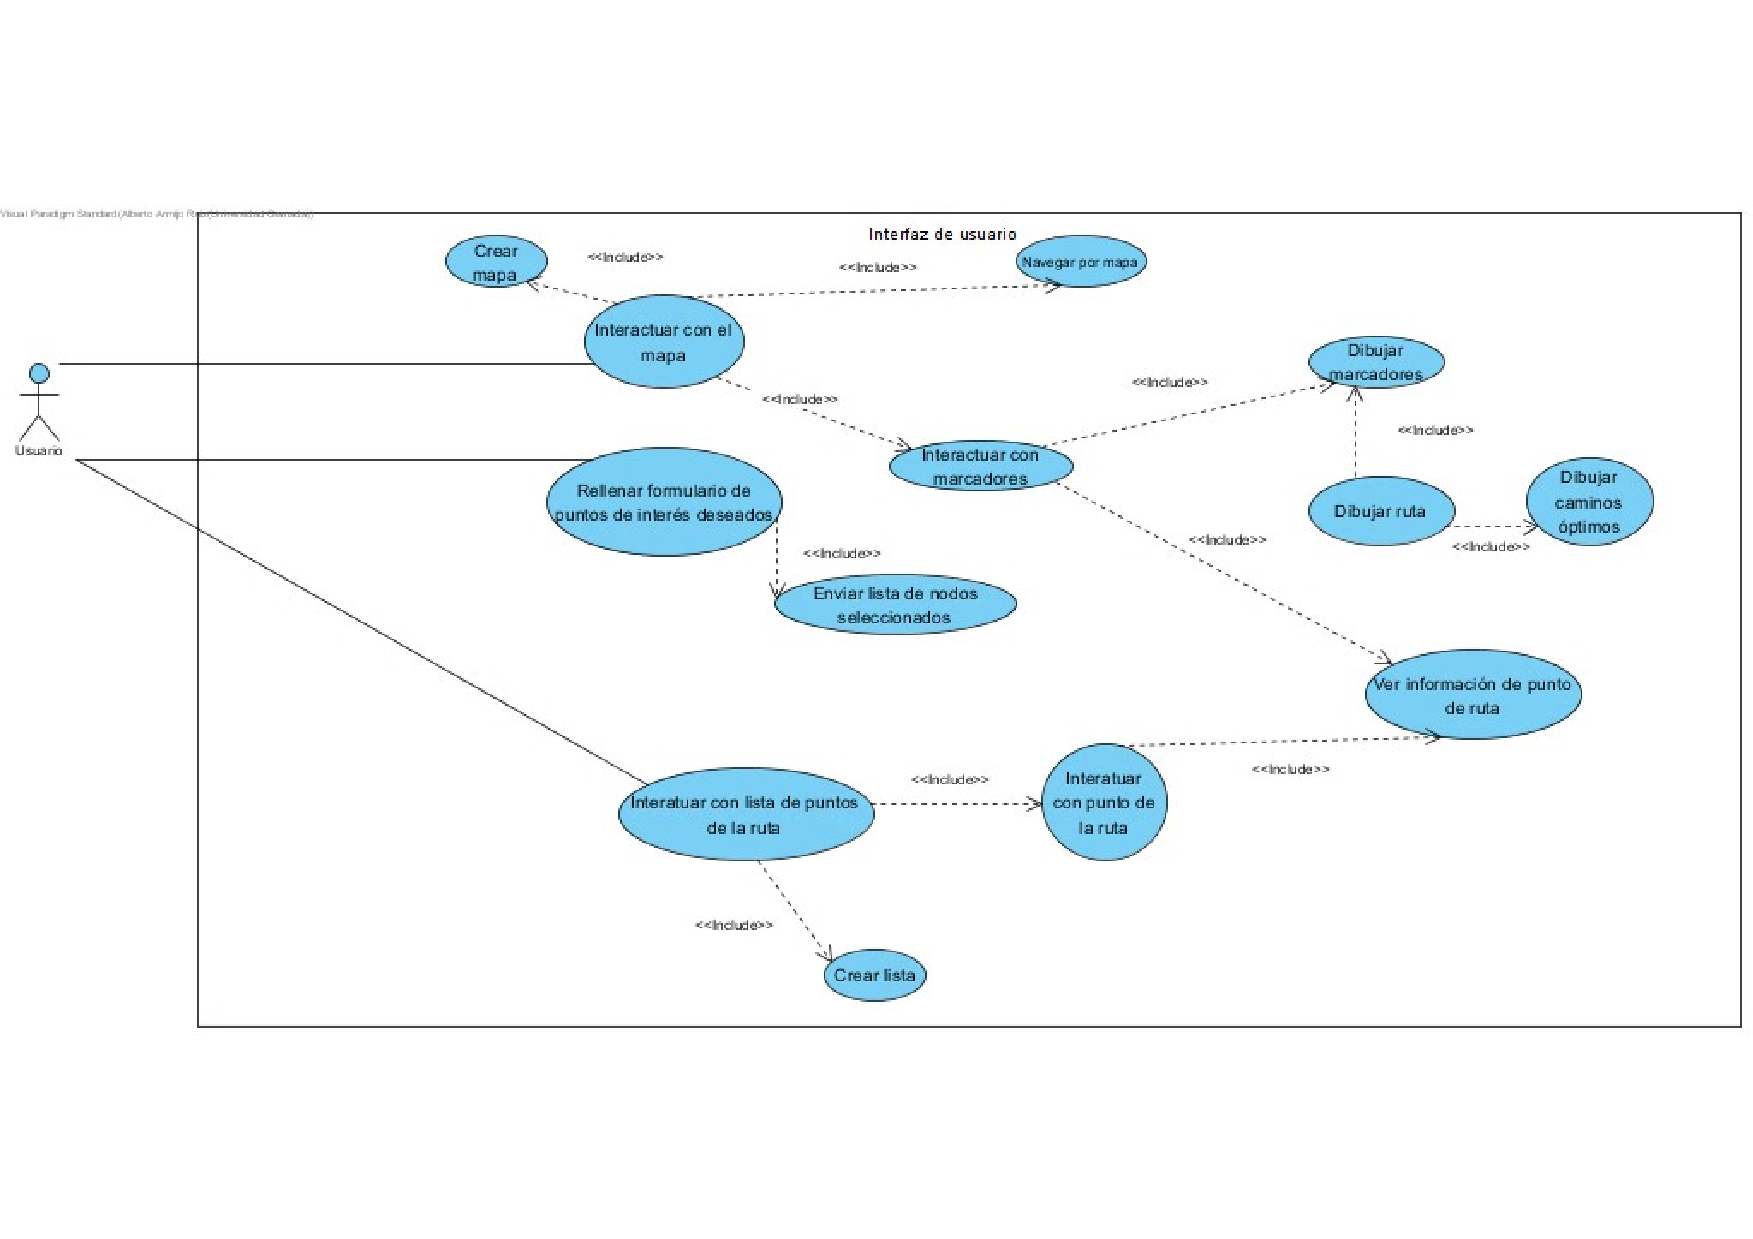
\includegraphics[scale=0.5]{imagenes/Interfaz.pdf}
	\caption{Diagrama de casos de uso de la interfaz de usuario}
	\label{fig:user_interface}
\end{figure}

\subsection[Aplicación]{Aplicación móvil}
\begin{figure}[H]
	\centering
	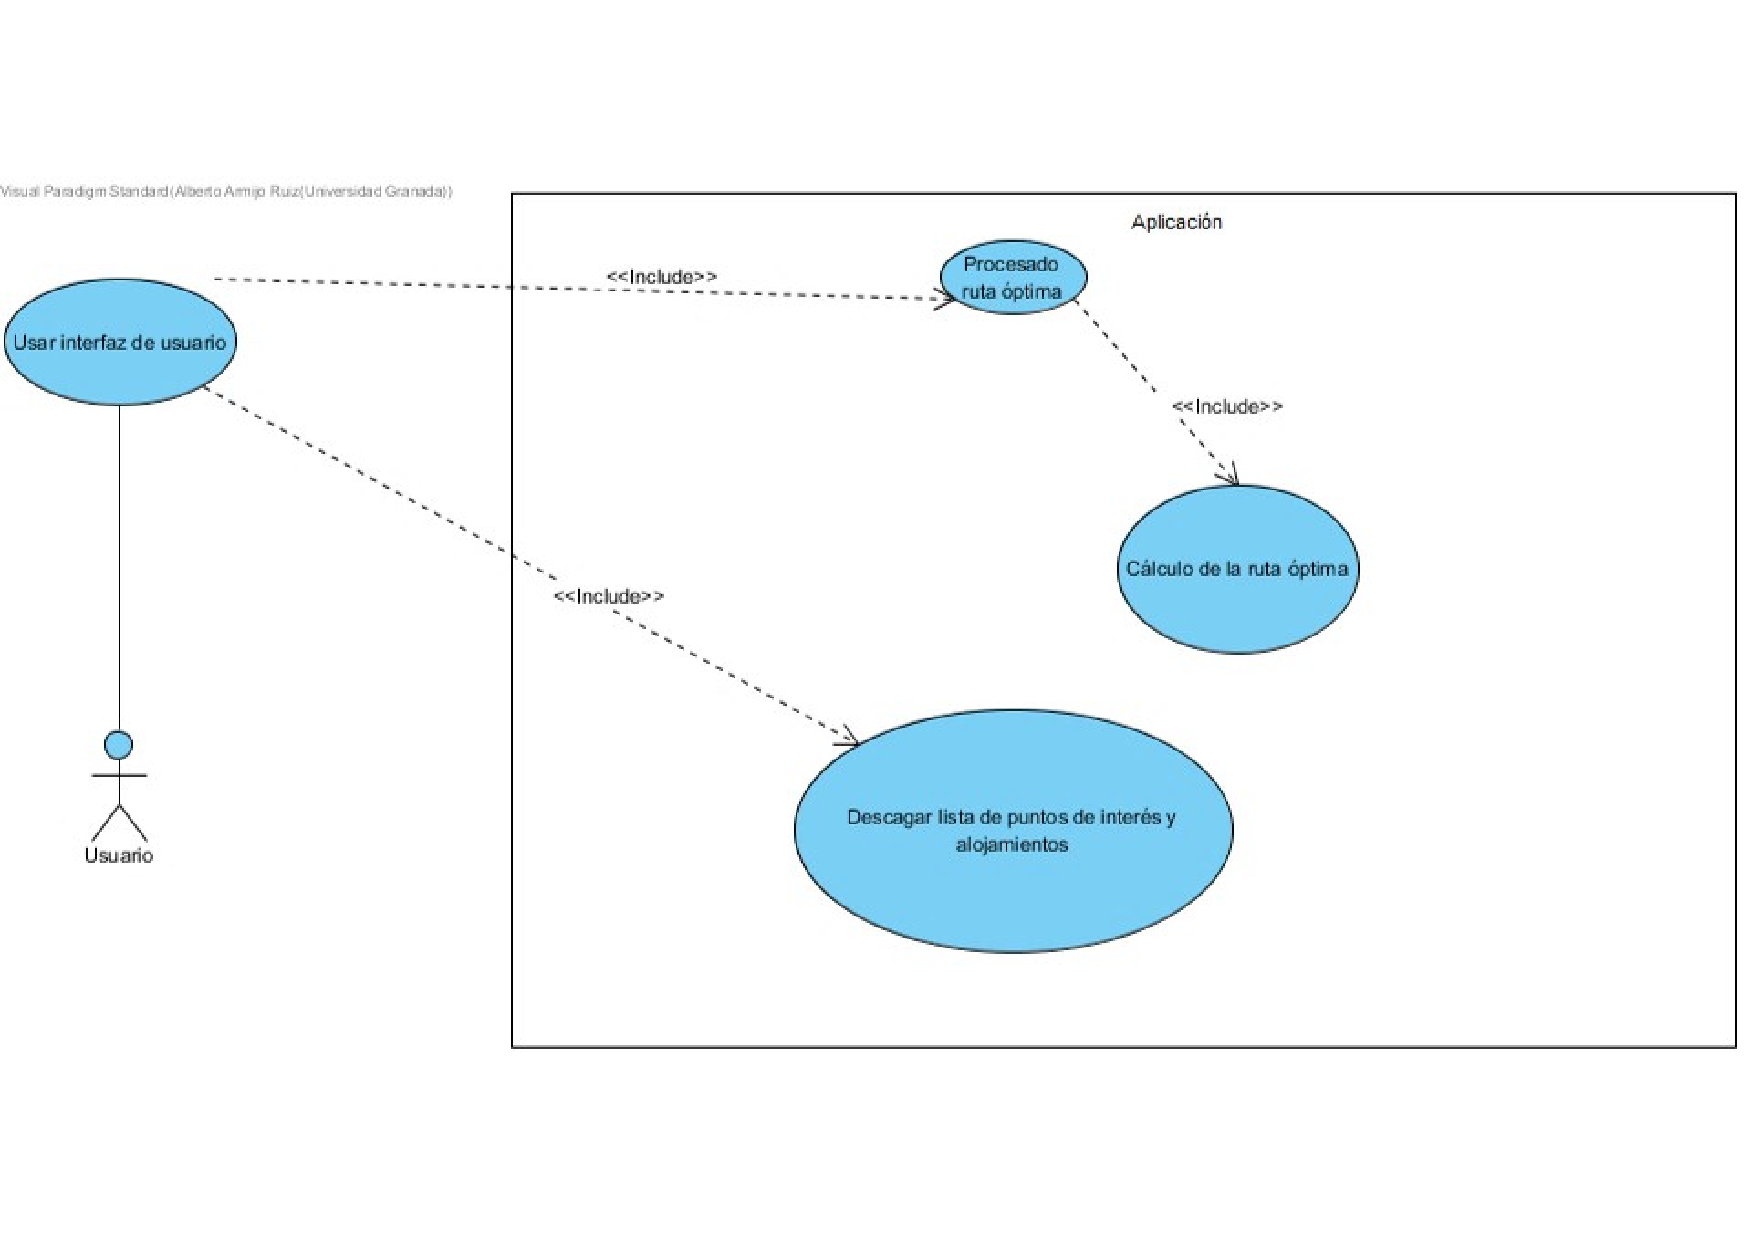
\includegraphics[scale=0.55]{imagenes/Aplicacion.pdf}
	\caption{Diagrama de casos de uso de la aplicación}
	\label{fig:app}
\end{figure}

\section[Fuente de los datos]{Fuente de los datos}
\subsection[OSM]{Open Street Map}
Ya que el objetivo de la aplicación fue crear rutas a partir de puntos de interés, se requirió obtener una lista con todos los puntos de interés y alojamientos disponibles en una ciudad con la suficiente información para que puedan ser usados para calcular rutas.\newline
Tras investigar diferentes posibilidades, se decidió utilizar OpenStreetMap, el cual es un proyecto colaborativo que permite crear mapas y editar los ya existentes.\newline
\begin{figure}[H]
	\centering
	
\includegraphics[scale=0.05]{imagenes/Openstreetmap_logo}
	\caption{Logo de OpenStreetMap}
	\label{fig:openstreetmap}
\end{figure}
OpenStreetMap tiene una web \cite{openstreetmap} en la cual puedes editar cualquiera de los puntos de interés que contiene el mapa o crear nuevos siempre que estés registrado. Además, cuenta con diferentes tipos de estructuras para representar edificios, carreteras, etc... OpenStreetMap utiliza tres tipos diferentes de información:\newline
\begin{itemize}
	\item Líneas: sirven para describir cualquier tipo de vía, como por ejemplo carreteras.
	\item Nodos: sirven para definir cualquier tipo de edificio, como por ejemplo farmacias o museos.
	\item Áreas: sirven para definir el espacio ocupado por un nodo, por ejemplo, un parque. Dichas áreas están formadas un conjunto de nodos que delimitan el área.
\end{itemize}
Al no estar disponible el acceso a la base de datos que contiene OpenStreetMap de forma directa se tuvo que buscar una API para poder obtener los datos.
\subsection[Overpass]{Overpass API}
Para obtener la información necesaria de OpenStreetMap, se necesitó buscar una API que permitiera obtener dicha información. Overpass es una API que permite hacer consultas sobre puntos de interés y que utiliza la información de OpenStreetMap para devolver la información sobre los puntos de interés. Dichas consultas pueden realizarse mediante urls. Las respuestas obtenidas por Overpass se devuelven en formato JSON, dentro de dicho fichero se encuentra un array llamado \enquote{elements} que contiene cada uno de los elementos. A continuación, se muestra una parte del fichero que devuelve Overpass para alojamientos y puntos de interés en Granada.\newline
\begin{lstlisting}[caption=Respuesta Overpass sobre alojamientos y puntos de interés en Granada]
{
"version": 0.6,
"generator": "Overpass API 0.7.54.13 ff15392f",
"osm3s": {
"timestamp_osm_base": "2018-02-27T10:23:02Z",
"copyright": "The data included in this document is from www.openstreetmap.org. The data is made available under ODbL."
},
"elements": [

{
"type": "node",
"id": 533647928,
"lat": 37.1734517,
"lon": -3.5888790,
"tags": {
"name": "Museo Manuel de Falla",
"tourism": "museum"
}
},
{
"type": "node",
"id": 940435771,
"lat": 37.1770011,
"lon": -3.5900734,
"tags": {
"name": "Museo de la Alhambra",
"tourism": "museum"
}
},
},
{
"type": "node",
"id": 1351215450,
"lat": 37.1765624,
"lon": -3.5897641,
"tags": {
"designation": "Museo de Bellas Artes",
"email": "museobellasartesgranada.ccul@juntadeandalucia.es",
"name": "Museo de Bellas Artes",
"tourism": "museum"
}
},
{
"type": "node",
"id": 1667155336,
"lat": 37.1625928,
"lon": -3.6066354,
"tags": {
"name": "Parque de las Ciencias",
"tourism": "museum"
}
},
...
{
"type": "node",
"id": 4029579625,
"lat": 37.1800207,
"lon": -3.5957336,
"tags": {
"addr:city": "Granada",
"addr:housenumber": "18",
"addr:postcode": "18010",
"name": "Makuto Guesthouse",
"tourism": "hostel",
"website": "http://makutohostel.com"
}
},
]
}
\end{lstlisting}

Para generar dicho fichero de salida, se deben ajustar ciertos parámetros dentro de la petición que se hace a Overpass. Para probar diferentes parámetros, se puede utilizar la herramienta de Overpass llamada Overpass-turbo.\newline
Overpass-turbo es una página web que contiene un mapa interactivo y una ventana donde nos permite escribir consultas a Overpass; desde ahí, se puede generar un script que encuentre todos los puntos de interés y alojamientos en una ciudad; después, dicho script puede exportarse como una petición en formato URL para utilizarla sin necesidad de utilizar Overpass-turbo. Dentro de dicho script debe especificarse los tipos de nodos que se quieren obtener, la información sobre los diferentes tipos de nodos se encuentra dentro de la documentación de OpenStreetMap \cite{openstreetmap_doc}.El script para obtener la información mostrada arriba es el siguiente. \newline
\begin{lstlisting}[caption=Script para encontrar todos los puntos de interés y alojamientos de una ciudad]
[out:json][timeout:100]; 

(node["place"="city"]["name"="Granada"]["is_in:province"="Granada"]["is_in:country"="Spain"];)->.ciudad; 

node["tourism"="museum"](around.ciudad:7000);
out;>;out;

node["tourism"="viewpoint"](around.ciudad:7000);
out;

// Catedrales.
node["building"="cathedral"](around.ciudad:7000);
out;

// Hoteles.
node["tourism"="hotel"](around.ciudad:7000);
out;

// Hotales.
node["tourism"="hostel"](around.ciudad:7000);
out;
\end{lstlisting}

\subsection[OSRM]{Open Source Routing Machine}
Como la aplicación necesita obtener la matriz de distancias entre los distintos puntos seleccionados por el usuario, se investigó para encontrar una herramienta que permitiera obtener dicha matriz a través de peticiones mediante URL.\newline
Tras probar con varias herramientas, se optó por usar OSRM \cite{osmr},la cual es de uso gratuito. OSRM permite hacer peticiones a sus servidores\cite{osmr_doc} o montar uno propio \cite{osmr_backend}.\newline
OSRM devuelve de sus peticiones un archivo JSON que contiene las distancias entre los puntos especificados en la petición, el tiempo que se tarda en llegar desde un punto a otro está guardado en un array llamado \enquote{durations}; cada elemento de dicho array contiene otro array con los tiempos desde dicho punto de interés al resto de puntos de interés. Un ejemplo de la salida de OSRM es el siguiente:
\begin{lstlisting}[caption=Salida de OSRM]
{"durations":
	[[0,245,165.9,165.9,165.9,44.9,162.3,130.6,130.6,44.9,56.2],
	[245,0,79.1,79.1,79.1,200.1,82.7,114.4,114.4,200.1,188.8],
	[165.9,79.1,0,0,0,121,3.6,35.3,35.3,121,109.7],
	[165.9,79.1,0,0,0,121,3.6,35.3,35.3,121,109.7],
	[165.9,79.1,0,0,0,121,3.6,35.3,35.3,121,109.7],
	[44.9,200.1,121,121,121,0,117.4,85.7,85.7,0,11.3],
	[162.3,82.7,3.6,3.6,3.6,117.4,0,31.7,31.7,117.4,106.1],
	[130.6,114.4,35.3,35.3,35.3,85.7,31.7,0,0,85.7,74.4],
	[130.6,114.4,35.3,35.3,35.3,85.7,31.7,0,0,85.7,74.4],
	[44.9,200.1,121,121,121,0,117.4,85.7,85.7,0,11.3],
	[56.2,188.8,109.7,109.7,109.7,11.3,106.1,74.4,74.4,11.3,0]],
	...
}
\end{lstlisting}

\subsection[Google Routes API]{Google Maps Directions API}
Dado que la aplicación debe mostrar el camino óptimo entre dos puntos seleccionados en la solución, se buscó una herramienta que lo calculara. Tras investigar y probar diferentes herramientas, se optó por utilizar Google Maps Directions API \cite{directions_api}.\newline
Esta herramienta permite hacer peticiones a un servidor y devuelve un archivo JSON que contiene la ruta que se debe seguir. Este archivo se debe procesar para obtener las polilíneas que represetan el camino entre dos puntos. Un ejemplo de este archivo es el siguiente.\newline
\begin{lstlisting}[caption=Salida de Google Maps Directions API]
{"routes" : [
...
"legs" : [
{
"distance" : {
"text" : "2.0 km",
"value" : 2044
},
"duration" : {
"text" : "25 min",
"value" : 1496
},
"end_location" : {
"lat" : 37.1622873,
"lng" : -3.6068922
},
"start_location" : {
"lat" : 37.1761203,
"lng" : -3.6025799
},
"steps" : [
{
"distance" : {
"text" : "0.1 km",
"value" : 115
},
"duration" : {
"text" : "1 min",
"value" : 75
},
"end_location" : {
"lat" : 37.1757377,
"lng" : -3.6037831
},

"polyline" : {
"points" : "w}{aFbs~TNx@VrAV|@Jb@"
},
"start_location" : {
"lat" : 37.1761203,
"lng" : -3.6025799
},
"travel_mode" : "WALKING"
},
{
"distance" : {
"text" : "0.4 km",
"value" : 354
},
"duration" : {
"text" : "4 min",
"value" : 252
},
"end_location" : {
"lat" : 37.1738268,
"lng" : -3.6069271
},

"polyline" : {
"points" : "k{{aFrz~T@Hp@nBP`@T\\j@p@fA|ADF~AtBfAlD"
},
"start_location" : {
"lat" : 37.1757377,
"lng" : -3.6037831
},
"travel_mode" : "WALKING"
},
}
\end{lstlisting}
%
%\chapter{Planificación}
\section[Objectivos]{Objetivos}
Los objetivos concretos que persigue este proyecto son los siguientes:
\begin{enumerate}
	\item Estudio del estado del arte de los sistemas de planificación de rutas con recomendaciones, y de los sistemas de información sobre puntos de interés en las ciudades.
	\item Definición y diseño de modelos y herramientas de recomendación de itinerarios ajustados a las necesidades y preferencias de los turistas.
	\item Validación de modelos y métodos, empleando pruebas y datos de puntos de interés en ciudades de interés turístico.
	\item Obtención de un prototipo software integrado en una aplicación para dispositivos móviles.
	\item Creación de documentación técnica, entregables y memoria final del proyecto.
	
\end{enumerate}

%
%\chapter{Análisis}
En este capítulo se explican los modelos teóricos y algorítmicos empleados para el diseño de las rutas y el desarrollo del sistema recomendador.
\section[Diseño de rutas turísticas]{Diseño de rutas turísticas}
Los problemas de diseño de rutas turísticas (Tourist Trip Design Problems, TTDP) consisten seleccionar los puntos de interés (point of interest, POI) a visitar por un turista atendiendo a sus restricciones y al beneficio o grado de satisfacción que produce su visita. El turista dispone en su estancia de un cierto número de días para organizar las visitas a los puntos de interés mediante rutas de duración limitada. Se parte de un conjunto de puntos disponibles a visitar de los que se conoce, el beneficio o grado de satisfacción, la duración de la visita y el intervalo de tiempo en el que puede realizarse. El beneficio total que intenta maximizar el turista es la suma de los beneficios obtenidos en cada visita.\newline
Los elementos que forman parte del modelo son:
\begin{itemize}
	\item Un conjunto de puntos de interés (POI), asociado a un índice $i, i=1,2,...,n$ y con los siguientes atributos:
	\begin{itemize}
		\item Una puntuación o beneficio $s_i$.
		\item Un tiempo de duración de la visita $r_i$.
		\item Un intervalo de tiempo $[e_i,l_i]$ dentro del que se puede realizar la visita.
	\end{itemize}
	\item Un punto de partida de cada una de las rutas denotado por $i=0$.
	\item Los tiempos de recorrido entre los pares de puntos $t_{ij}, i=0,1,...,n$.
	\item Un tiempo máximo $T_{max}$ de duración total de la ruta del día considerando los tiempos de viaje, visita y espera en los POI.
	\item Una función objetivo $max \sum_{i=1}^{n}s_iy_i^k$ \newline
	En la que $y_i$ corresponde a una variable de visita para cada uno de los puntos de interés $i, i=1,...,n$. Dicha variable es binaria, teniendo como valor 1 si el punto de interés $i$ es visitado en la ruta y un 0 si no se visita.
\end{itemize}
El problema de optimización coincide con el Team Orienteering Problem with Time Windows (TOPTW) que se ha estudiado en la literatura científica con algunas modificaciones. Se consideran puntos de interés museos, miradores, catedrales, mezquitas, etc... de la ciudad que el usuario elija.
\section[Heurísticas del diseño]{Heurísticas del diseño}
Para dar soluciones de alta calidad al problema de optimización planteado se ha elegido la metaheurística constructiva GRASP (Greedy Randomized Adaptive Search Procedure) que comprende dos fases: una fase contructiva y otra de búsqueda local. En la fase constructiva se genera una solución partiendo de una ruta vacía a la que se va añadiendo puntos de interés desde una Lista Restringida de Candidatos (Restricted Candidate List, RCL en inglés) de forma aleatoria hasta que no se puedan añadir nuevos puntos a la ruta. En la fase de búsqueda local se reemplaza la solución obtenida en la parte constructiva por la mejor de sus soluciones vecinas si existe mejora. Estas dos fases se ejecutan un cierto número de iteraciones.

Ahora se mostrará el pseudocódigo del algoritmo, y de cada una de las fases en inglés.
\vspace{0.06in}

\begin{algorithm}
	\caption{Pseudocódigo algoritmo GRASP}
	\label{alg:grasp}
\begin{algorithmic}
	\Function{GRASP}{maxIterations,sizeRCL}
	\State $ readInput() $
	\For{$i=1$ to maxIterations}
		\State $ solution \gets GRASPConstructPhase(sizeRCL)$
		\State $ solution \gets LocalSearch(solution)$
		\If{$solution \geq bestSolution$}
			\State $ bestSolution \gets solution$
		\EndIf
	\EndFor
	
	\State \textbf{return} $bestSolution$
	\EndFunction
\end{algorithmic}
\end{algorithm}

\vspace{0.06in}
Para la parte constructiva del algoritmo, primero crearemos una lista de candidatos (CL), la cual tiene un tamaño igual al de la lista de puntos de interés que queden disponibles. Dicha lista de candidatos contiene la posición dentro de la lista de puntos de interés y la puntuación que tiene dicho punto de interés según las preferencias elegidas por el usuario. La forma de puntuar a cada punto de interés se hace de la siguiente manera:\newline
$ \frac{1}{time\_between(poi_{i-1},poi_i)}\sum_{j=1}^{n}c_j$ \newline
Donde time\_between(x,y) representa el tiempo que hay entre el punto de interés x y el y. $poi_{i-1}$ representa el último punto de interés que hemos incluido en la solución y $poi_i$ al punto de interés que estamos evaluando; $c_j$ es cada uno de las preferencias posibles sobre los puntos de interés, es decir, si se ha seleccionado museos como preferencia y el punto de interés $i$ es un museo, $c_j$ devolverá uno, es caso contrario es cero.\newline
Una vez hemos calculado la lista de candidatos, se crea la lista restringida de candidatos con los puntos de interés mejor valorados, esta es de tamaño sizeRCL. Una vez hemos obtenido la lista de candidatos restringida, elegimos uno de los puntos de interés de forma aleatoria y lo introducimos dentro de la solución. Este proceso se repite hasta que no se puedan introducir más puntos de interés dentro de la solución. El pseudocódigo de este algoritmo es el siguiente.
\vspace{0.06in}
\begin{algorithm}
	\caption{Pseudocódigo algoritmo GRASPConstructPhase}
	\label{alg:grasp_contruct}
	\begin{algorithmic}
		\Function{GRASPConstructPhase}{sizeRCL}
		\State $solution.add(first\_node)$
		\While{is posible to visit POIs}
			\For{each poi in POIs}
				\State $value \gets f(poi)$
				\State $cl.add([value,i])$
			\EndFor
			\State Create rcl with the top sizeRCL duos in cl
			\State Select a random duo from rcl.
			\State Update solution adding the poi in the position i.
		\EndWhile
		\State \textbf{return} $solution$
		\EndFunction
	\end{algorithmic}
\end{algorithm}

\vspace{0.06in}
Para la fase de optimización se utilizará el algoritmo de búsqueda local, dicho algoritmo busca la mejor solución posible entre la solución actual y los vecinos de esta. Una solución vecina es aquella que intercambie dos puntos de interés dentro de la solución, por ejemplo, el segundo por el cuarto. El procedimiento es el siguiente, se generan todos los posibles vecinos de la solución, y por cada uno de ellos se comprueba si la valoración de dicha solución vecina es mejor que la mejor solución actual; finalmente se devuelve la mejor solución encontrada. El pseudocódigo del algoritmo es el siguiente.
\begin{algorithm}[H]
	\caption{Pseudocódigo algoritmo LocalSearch}
	\label{alg:local_search}
	\begin{algorithmic}
		\Function{LocalSearch}{solution}
		\ForAll{neighbor\_solution of solution}
		\If{$neighbor\_solution \geq solution$}
			\State $solution \gets neighbor_solution$
		\EndIf
		\EndFor
		\State \textbf{return} $solution$
		\EndFunction
	\end{algorithmic}
\end{algorithm}



%
%\chapter{Diseño}
En este capítulo se detalla la arquitectura del sistema.
\section[Diagrama de clases]{Diagrama de clases}
En este apartado se mostrarán los diagramas de clases de los elementos más importantes de la aplicación.\newline

La primera figura que se muestra es el diagrama de clases del Fragment \enquote{TypesFragment} \ref{fig:fragment_diagram}. Dicho diagrama de clases muestra las siguientes clases:
\begin{itemize}
	\item La clase \textbf{TypesFragment}:esta clase es la encargada de comunicar los elementos gráficos que se encuentra dentro de la lista de alojamientos y puntos de interés, también del botón que inicia el algoritmo de búsqueda de la ruta óptima.
	\item La clase \textbf{TypesRecyclerFragment}: es la encargada de manejar la lista de alojamientos y puntos de interés, además devuelve los elementos seleccionados en la lista al iniciar la búsqueda de la ruta. También se encarga de gestionar la interfaz gráfica de la lista.
	\item La clase \textbf{CityNodesViewHolder}: es la encargada de gestionar los elementos gráficos de los puntos de interés o los alojamientos de forma individual.
	\item La clase \textbf{TypeViewHolder}: es la encargada de gestionar los elementos gráficos de los tipos que aparecen en la lista de alojamientos y puntos de interés.
	\item La clase \textbf{CityNode}: clase que contiene toda la información importante sobre un alojamiento o punto de interés que se muestra en la lista.
	\item La clase \textbf{TypeOfNode}: clase que contiene la información sobre un tipo de nodo de interés.
\end{itemize}
\vspace{0.06in}
En la segunda figura  \ref{fig:main_activity_diagram}, se muestra el diagrama de clases de la actividad principal de la aplicación. Las clases que se muestran en el diagrama son las siguientes:
\begin{itemize}
	\item La clase \textbf{MapsActivity} es la clase clase principal y gestiona el mapa que se muestra y se comunica con la clase \textbf{TypesFragment} para obtener los nodos seleccionados. Esta clase contiene vectores que almacenan información sobre los marcadores que aparecen en el mapa. Dicha información se utiliza también para obtener la matriz de distancias. También contiene otros vectores para almacenar la información contenida en la solución, dichos vectores se utilizan para mandar la información de la solución a la actividad ResultActivity.
	\item La clase \textbf{DownloadFileFromURL}: se encarga de descargar y guardar la información que devuelven las peticiones a los servidores sobre alojamientos, puntos de interés, rutas y matriz de tiempos entre puntos de interés. Esta clase hereda de la clase AsyncTask, lo cual le permite ejecutarse en segundo plano sin que afecte al rendimiento de la interfaz de usuario.
	\item La clase \textbf{jsonProcessor} se encarga de procesar la información que se ha guardado en ficheros tras ser descargada. Esta clase utiliza la clase \textbf{JsonParser} para procesar los archivos. Además, también hereda de la clase AsyncTask por lo que se ejecuta en segundo plano.
	\item La clase \textbf{JsonParser} se encarga de procesar archivos JSON y devuelve la información contenida en los archivos en estructuras que la aplicación puede manipular.
	\item La clase \textbf{SendNodes} se encarga de obtener la matrix de distancias entre los puntos de interés selecionados. Para ello utiliza las clases \textbf{DownloadFileFromURL} y\textbf{ jsonProcessor}, también se ejecuta en segundo plano debido a que hereda de la clase AsyncTask.
	\item La clase\textbf{ FindSolution} se encarga de ejecutar en segundo plano el algoritmo de búsqueda de rutas y de mandar la solución a la siguiente actividad. Para ello hace uso de la clase \textbf{PathFinder} y la clase \textbf{Solution}.
	\item La clase \textbf{PathFinder} es la clase que contiene el algoritmo de búsqueda de rutas. Dicha clase obtiene la solución al problema mediante un algoritmo Greedy y devuelve un objeto de la clase \textbf{Solution}.
	\item La clase \textbf{Solution} es la que clase que contiene una solución al problema. Esta clase cuenta con un vector que almacena los identificadores de los puntos de la solución, así como dos vectores que almacenan las horas de entrada y de salida de cada uno de los puntos de la solución.
\end{itemize}
\vspace{0.06in}
En la tercera figura \ref{fig:models_diagram}, se muestra el diagrama de clases del paquete models; dicho paquete está formador por clases que se utilizan para modelar diferentes estructuras dentro del proyecto. Las clases que aparecen en el diagrama son las siguientes:
\begin{itemize}
	\item La clase \textbf{Solution}: clase que contiene una solución al problema. Contiene vectores para almacenar identificadores y horarios de entrada y salida de los lugares por los que pasa la solución.
	\item La clase \textbf{ModelNode}: clase genérica que se utiliza para poder mostrar elementos tanto de la clase \textbf{CityNode} y \textbf{TypeOfNode}; ambas clases están explicadas en la descripción del primer diagrama de clases.
	\item La clase \textbf{SolutionNode}: clase que contiene el nombre, el horario de entrada y salida de un nodo de la solución. Esta clase se utiliza para encapsular los nodos de la solución y acceder a los datos a la hora de mostrar la lista de la solución.
\end{itemize}
\vspace{0.06in}
La cuarta figura \ref{fig:result_activity_diagram} muestra el diagrama de clases de la Activity ResultActivity, dicha Activity se muestra cuando se obtiene una solución. Las clases que se muestran en el diagrama son las siguientes:
\begin{itemize}
	\item La clase \textbf{ResultActivity}. Esta clase se ocupa de leer los datos mandados por la actividad principal y procesarlos para comunicarselos a la clase \textbf{SolutionFragment}.
	\item La clase \textbf{SimpleFragmentPagerAdapter}. Esta clase se ocupa de ver el número de soluciones que se han encontrado y crear un objeto de la clase \textbf{SolutionFragment} para mostrar cada una de ellas.
	\item La clase SolutionFragment. Esta clase se ocupa de mostrar en un mapa los marcadores de la solución y la lista con la información específica de cada uno de los marcadores. Además se ocupa de calcular el camino entre los distintos marcadores de la solución.
\end{itemize}
\vspace{0.06in}
Por último, en la quinta figura \ref{fig:solution_recycler_diagram} se muestra el diagrama de clases de la clase \textbf{SolutionFragment}. A continuación se describen cada una de las clases que se muestran en el diagrama:
\begin{itemize}
	\item La clase \textbf{SolutionFragment} se ha definido en la figura \ref{fig:result_activity_diagram} anterior. Es la encargada de gestionar todas las vistas que muestran la solución.
	\item La clase \textbf{FindRoutes}. Esta clase se encarga de mandar una petición a un servidor para obtener la ruta óptima entre los nodos de la solución y procesarla, después manda la información procesada a la clase \textbf{SolutionFragment} para que dibuje la ruta.
	\item La clase \textbf{SolutionRecyclerAdater} se encarga de manejar la lista con los nodos de la solución y de mostrarlos en una lista.
	\item La clase \textbf{SolutionNode}. Es una clase que contiene la información sobre un nodo de la solución.
	\item La clase \textbf{SolutionNodeViewHolder}. Es una clase que utiliza la información de un objeto de la clase \textbf{SolutionNode}  y la muestra dentro de la lista que gestiona la clase \textbf{SolutionRecyclerAdapter}.
\end{itemize}
\begin{figure}[H]
	\centering
	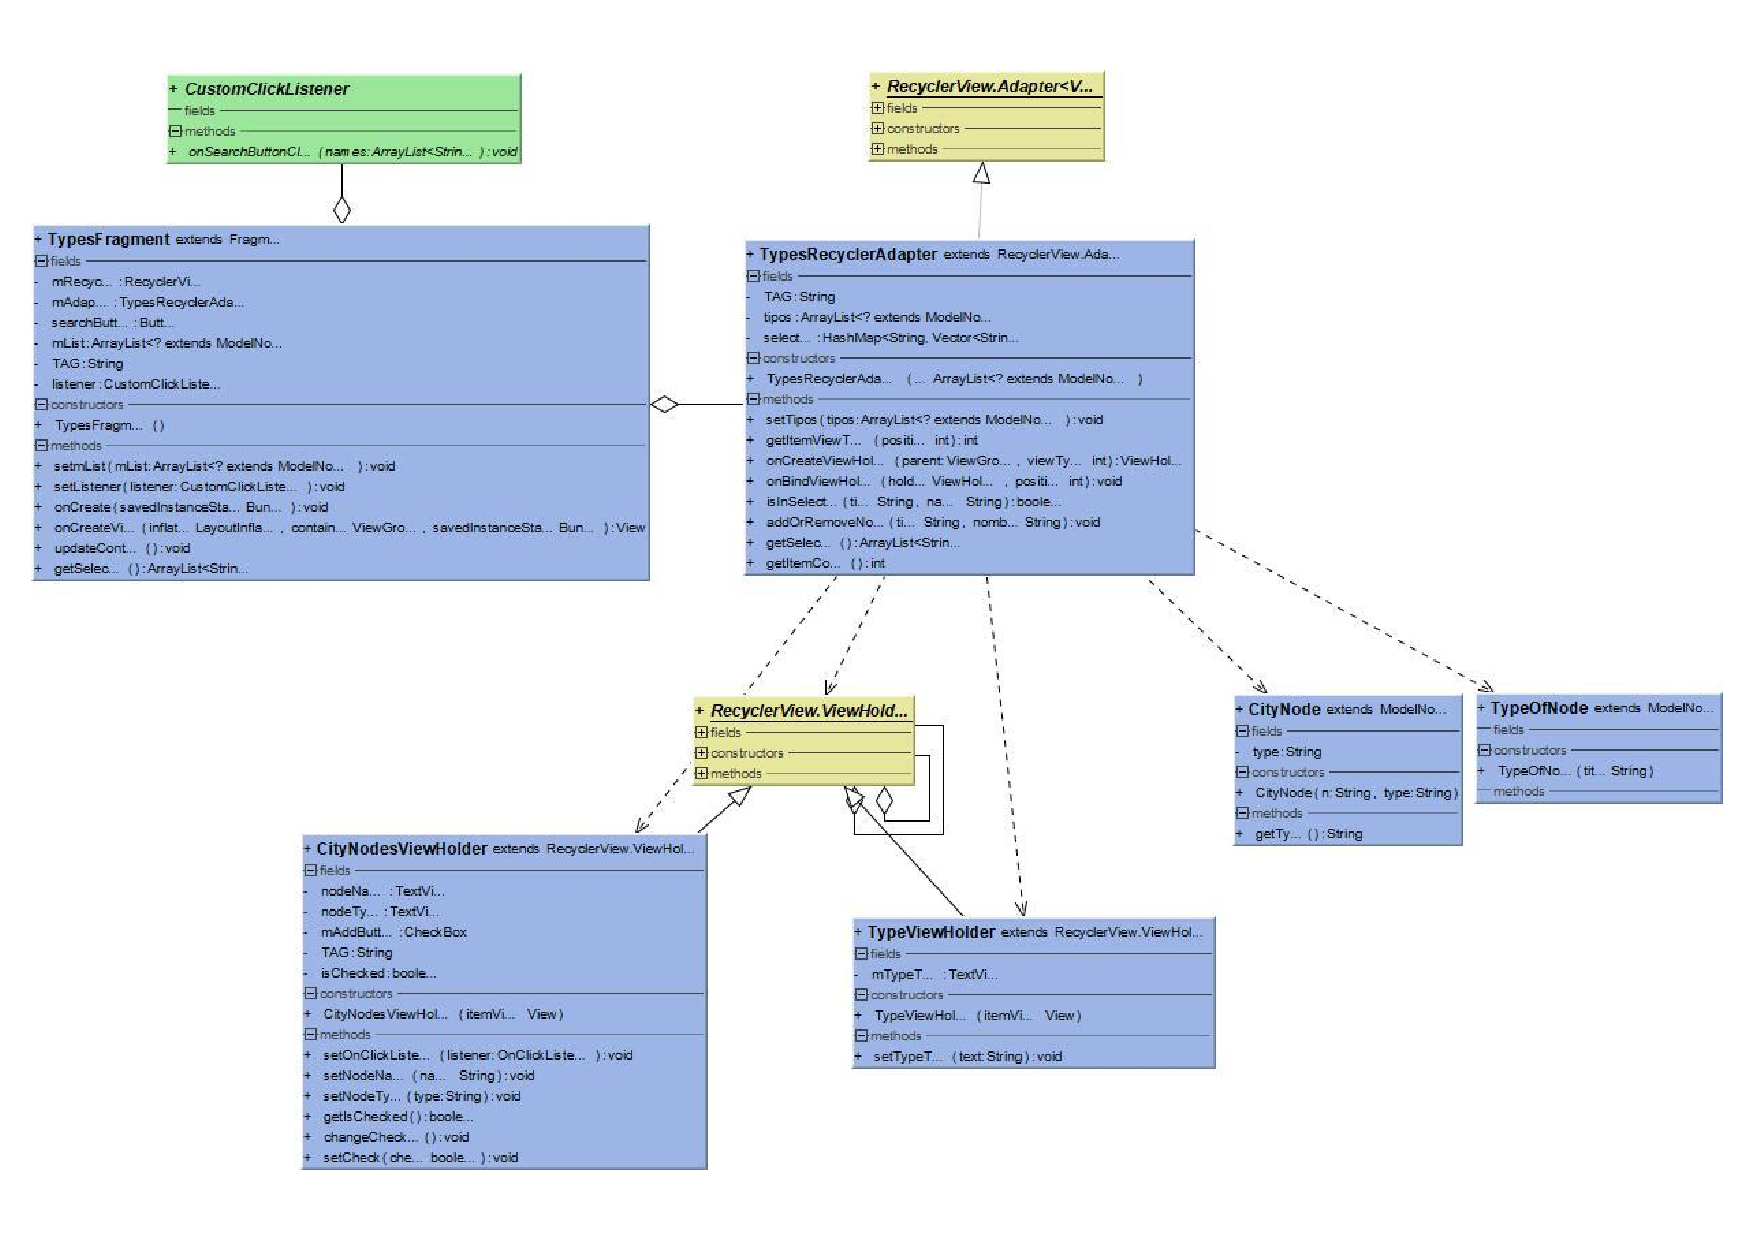
\includegraphics[scale=.8,angle=90]{imagenes/fragment_class_diagram.pdf}
	\caption{Diagrama de clases del \textbf{TypesFrament} }
	\label{fig:fragment_diagram}
\end{figure}
\begin{figure}[H]
	\centering
	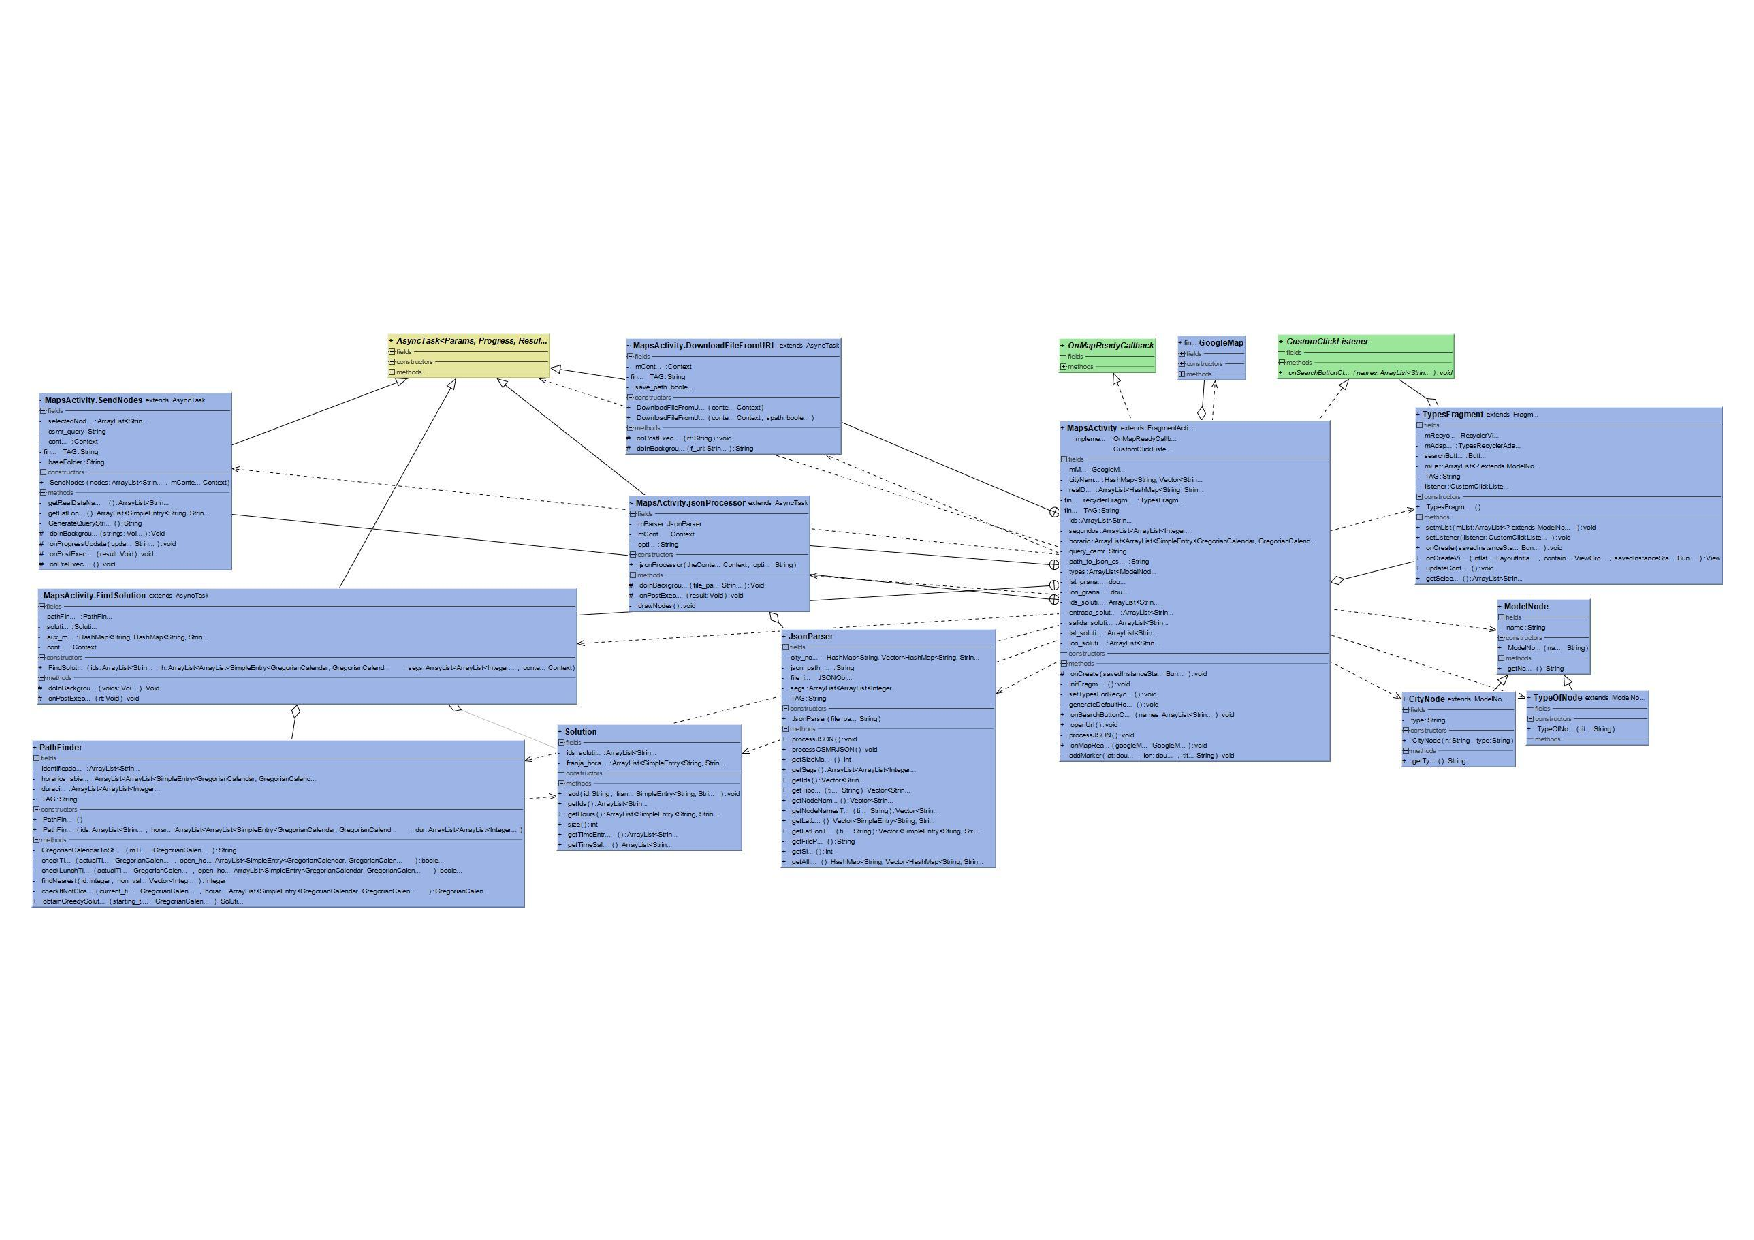
\includegraphics[scale=.8,angle=90]{imagenes/main_activity_class_diagram.pdf}
	\caption{Diagrama de clases de la actividad principal \ref{fig:anexo_diagrama_main_activity} }
	\label{fig:main_activity_diagram}
\end{figure}
\begin{figure}[H]
	\centering
	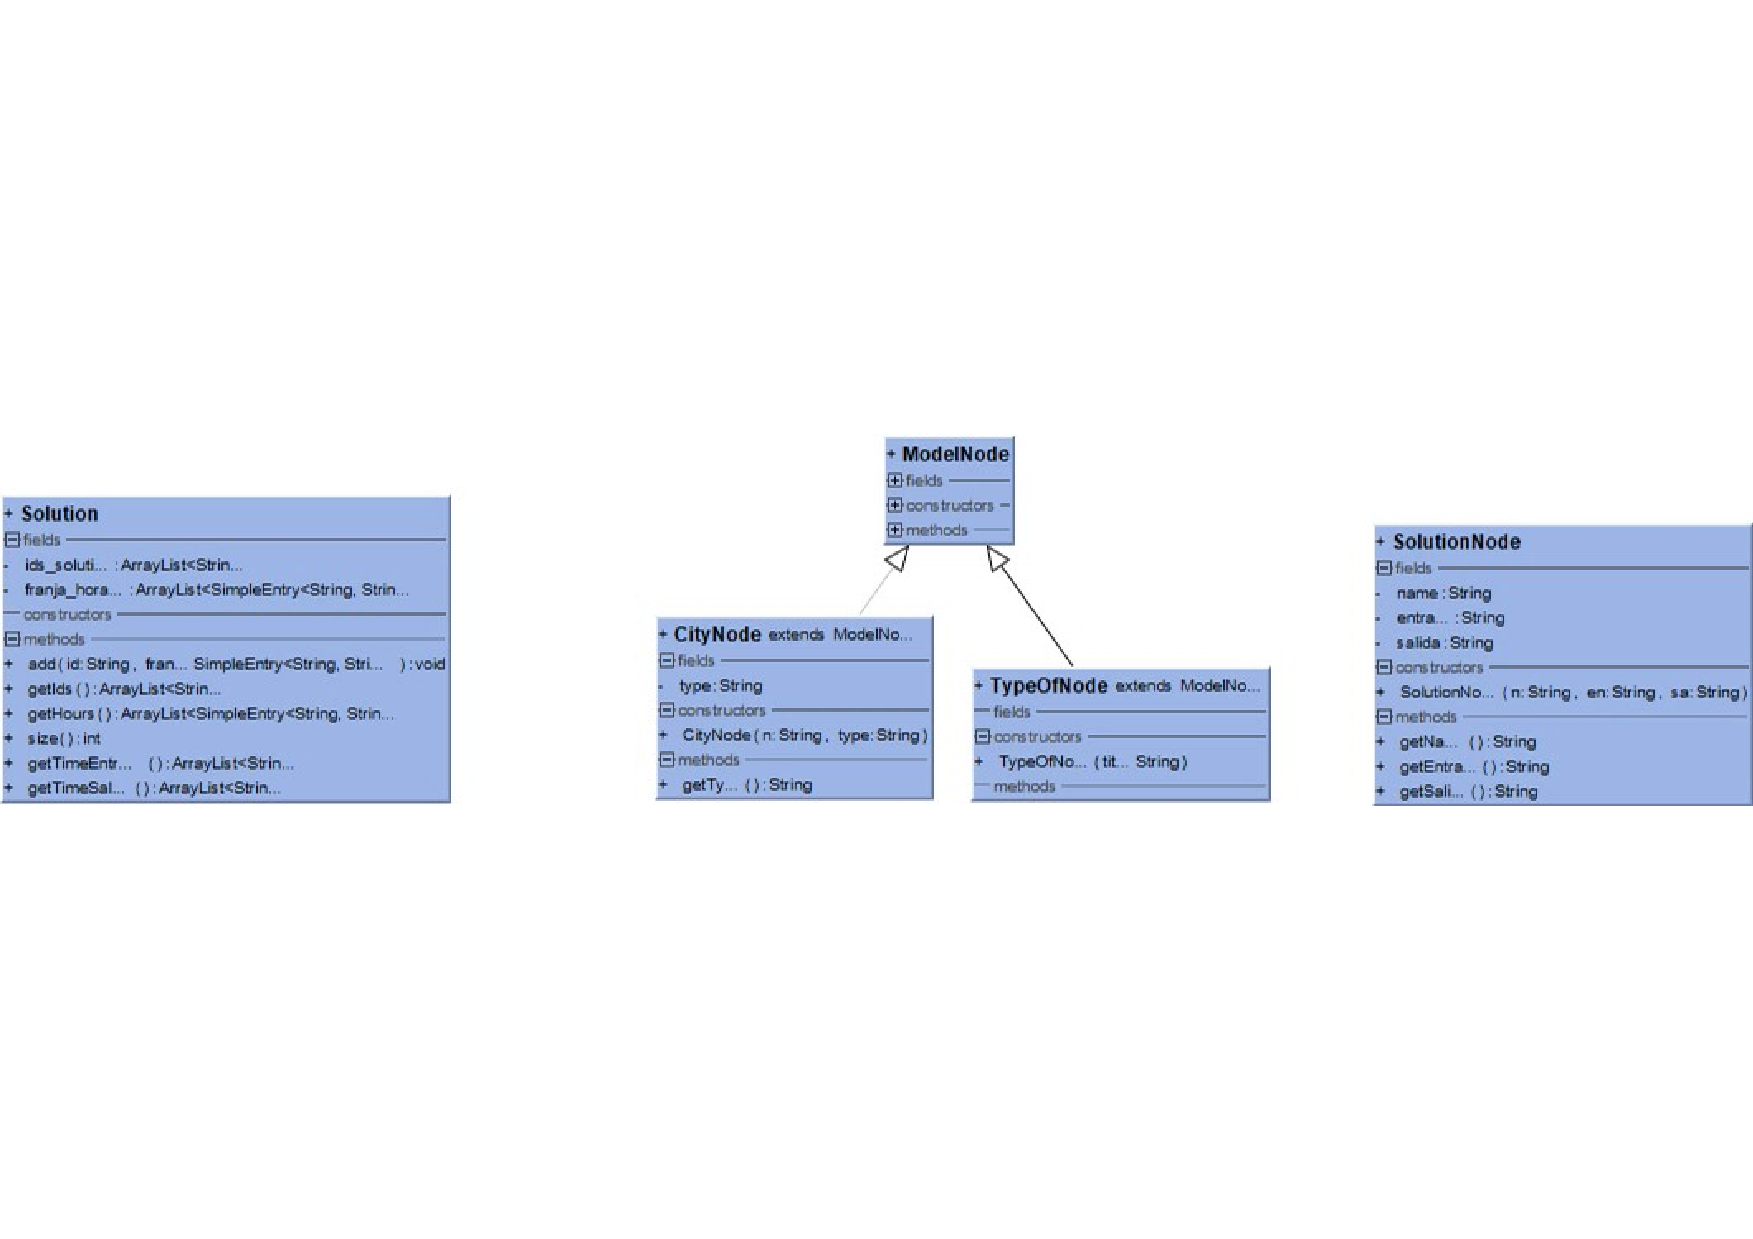
\includegraphics[scale=0.8,angle=90]{imagenes/models_package.pdf}
	\caption{Diagrama de clases del paquete \textbf{models}}
	\label{fig:models_diagram}
\end{figure}

\begin{figure}[H]
	\centering
	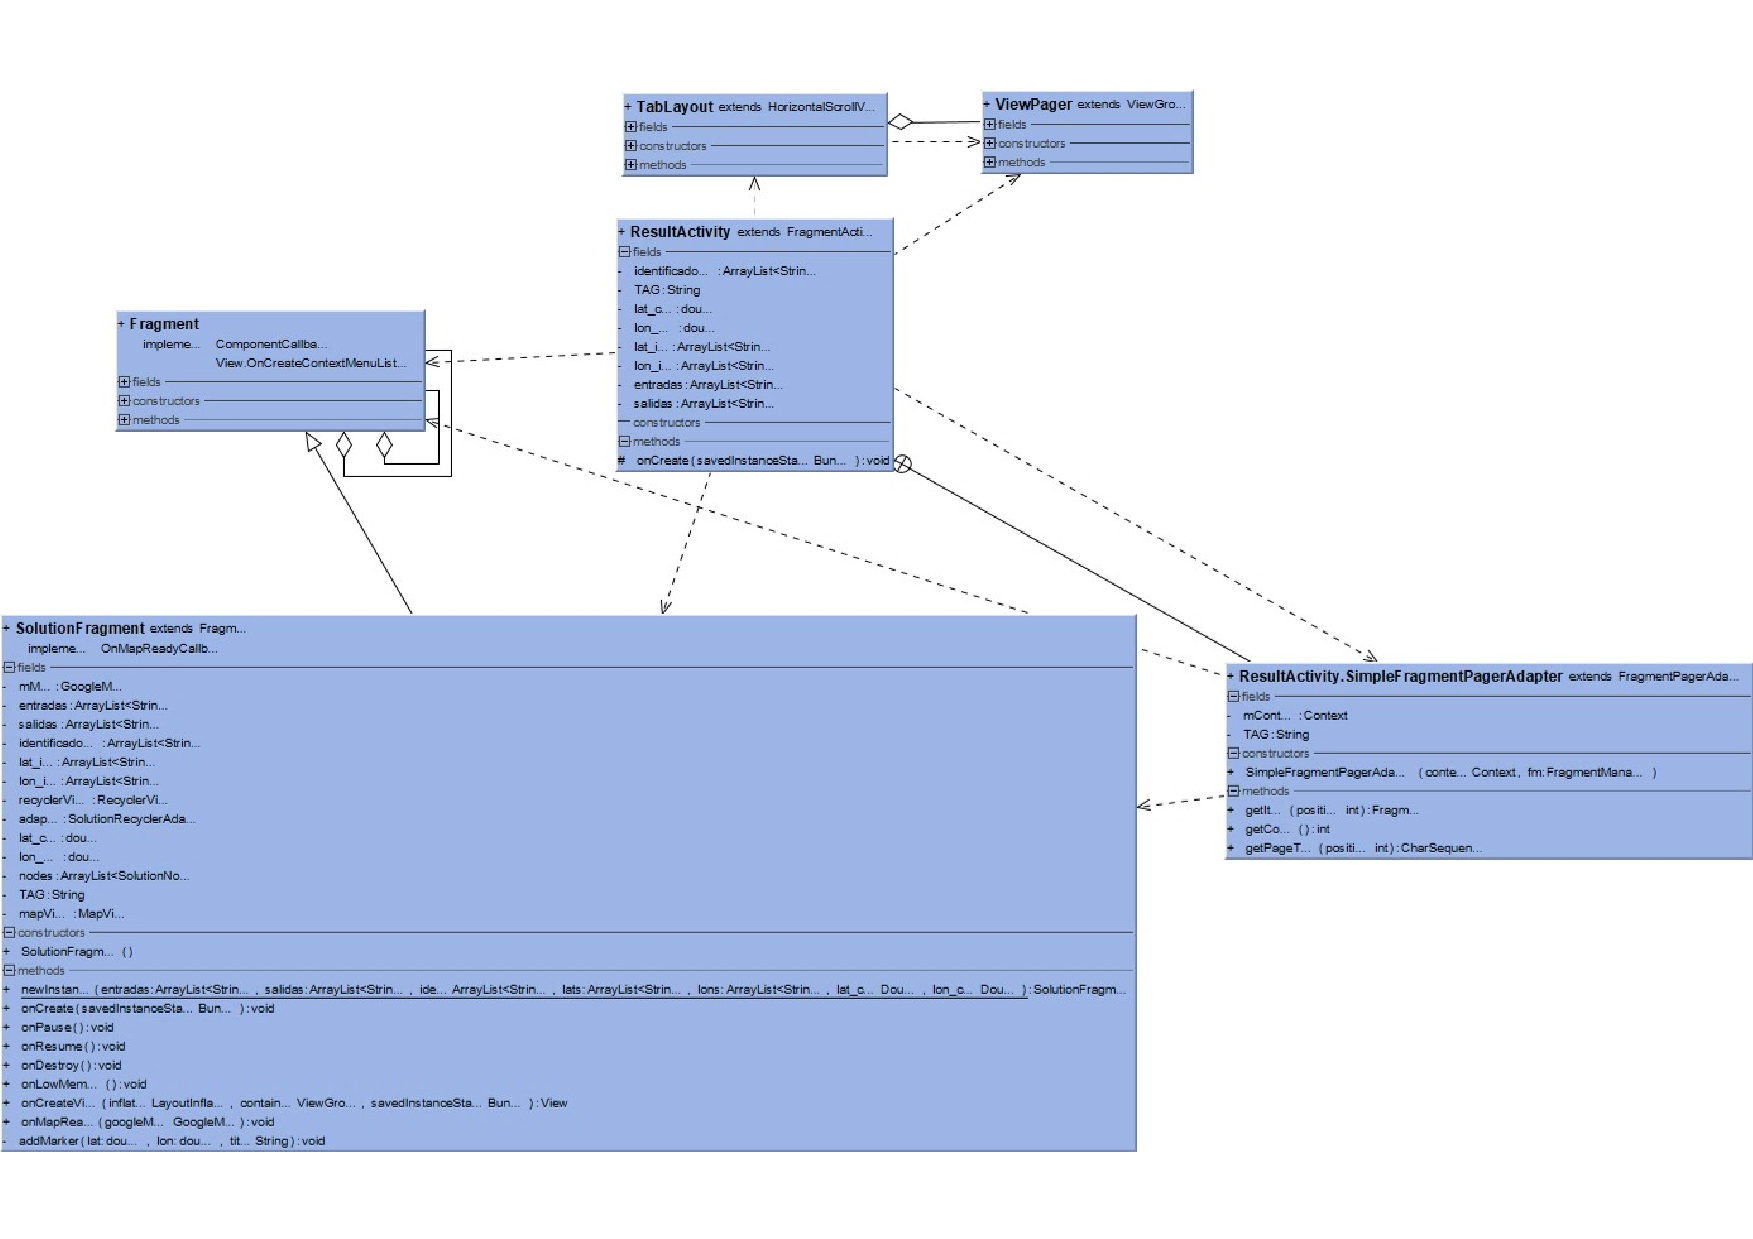
\includegraphics[scale=0.8,angle=90]{imagenes/result_activity.pdf}
	\caption{Diagrama de clases del activity \textbf{ResultActivity}}
	\label{fig:result_activity_diagram}
\end{figure}
\begin{figure}[H]
	\centering
	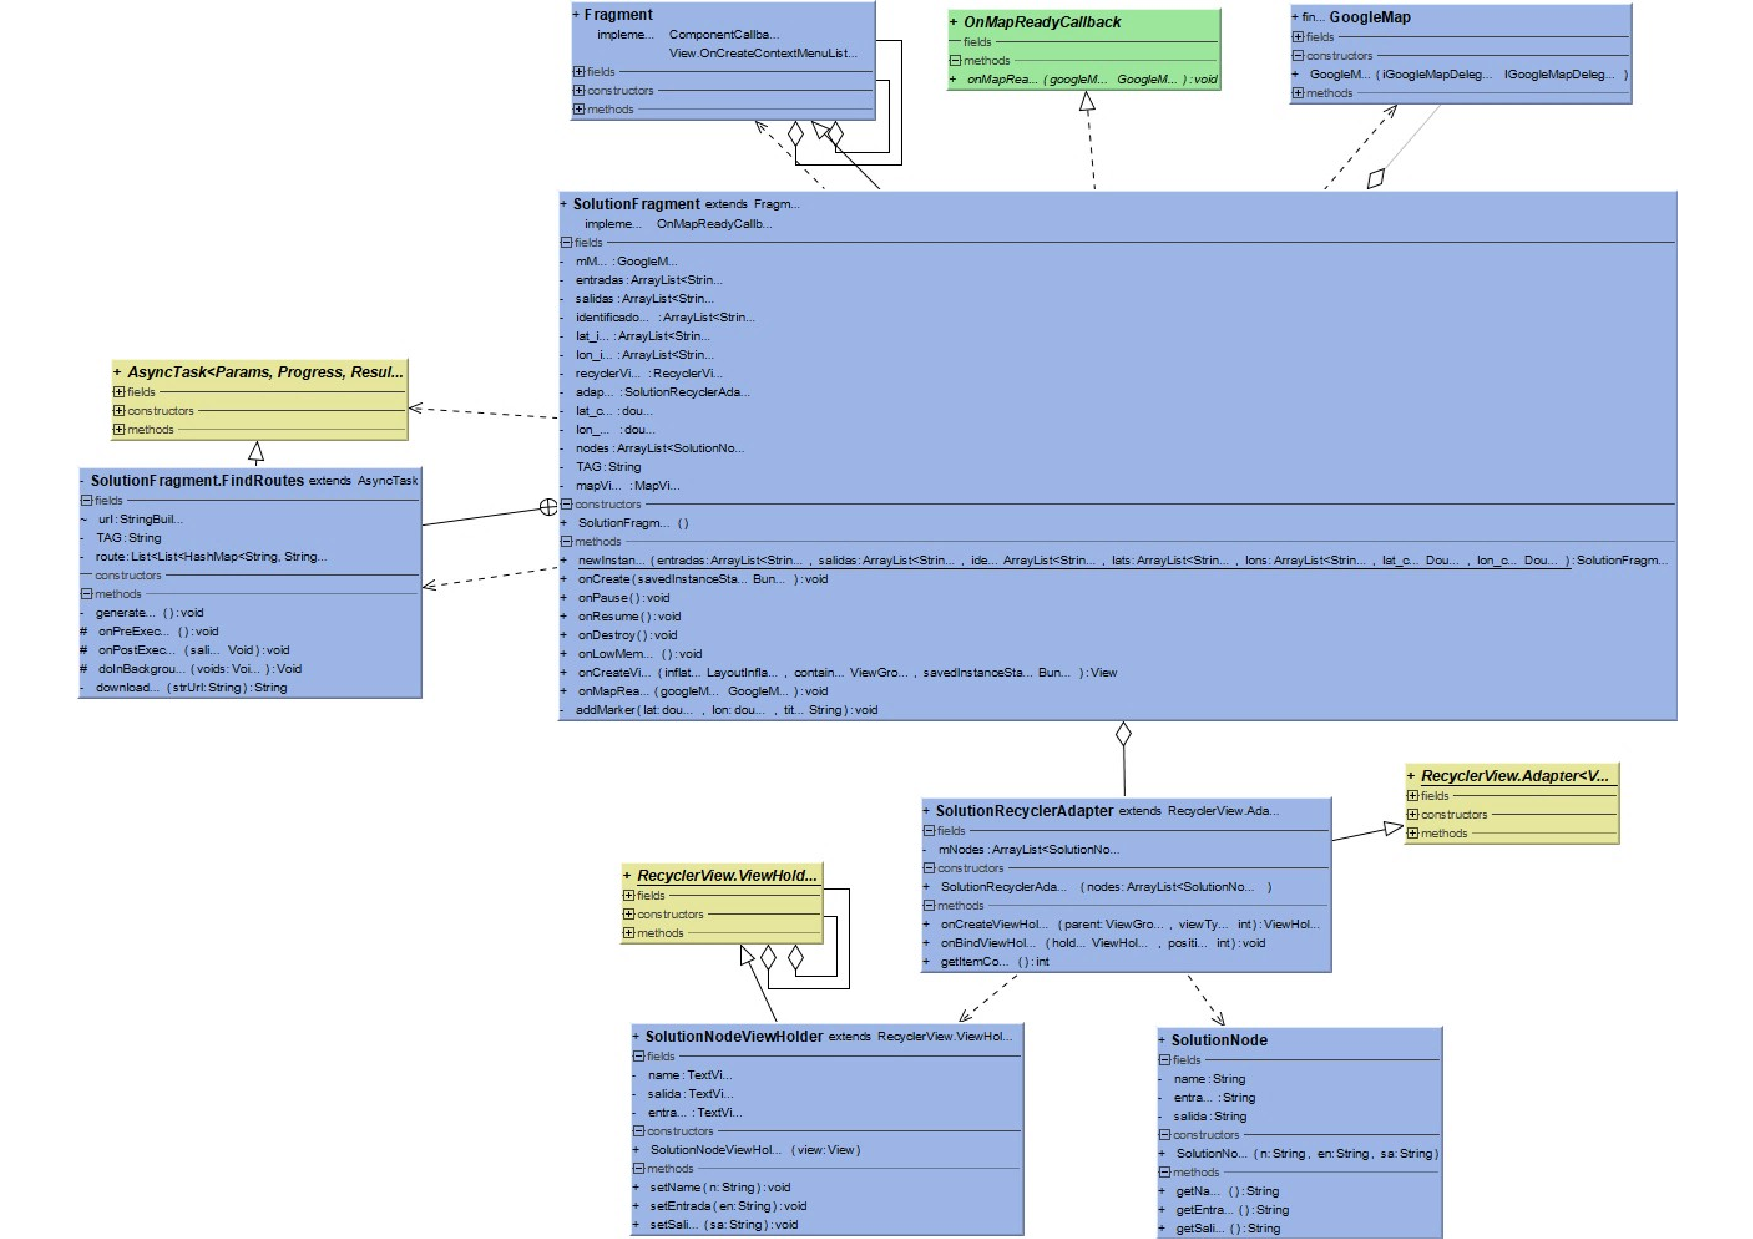
\includegraphics[scale=0.8,angle=90]{imagenes/result_fragment.pdf}
	\caption{Diagrama de clases de la clase \textbf{SolutionFragment}}
	\label{fig:solution_recycler_diagram}
\end{figure}


\section[Interfaz de Usuario]{Interfaz de Usuario}

A continuación se mostrarán todos los elementos que conforman la interfaz de usuario de la aplicación.\newline

Lo primero que se muestra es la actividad principal, esta cuenta con un mapa por el que se puede navegar y una lista de alojamientos y puntos de interés, entre los cuales el usuario puede elegir un alojamiento y el número de puntos de interés que desee; esto se puede encontrar en las figuras \ref{fig:main_activity_map}\ref{fig:main_activity_list}.\newline

Para poder ver la lista, se debe deslizar la pestaña \enquote{Sitios interesantes} hacia arriba, así tendremos acceso a la lista completa, para explorar todos los alojamientos y puntos de interés, debemos hacer scroll hacia arriba sobre la lista. Dicha lista muestra primero los alojamientos y tras estos los puntos de interés, que se organizan en \enquote{Museos}, \enquote{Miradores} y \enquote{Monumentos}.\newline

Dentro la lista, cada uno de los elementos contiene un caja en la que se puede pulsar para seleccionar o deseleccionar de dicho elemento. Dentro de las vistas de los tipos de punto de interés, se encuentra también una caja, dicha caja permite seleccionar o deseleccionar todos los puntos de interés de ese tipo.\newline

Tras elegir el alojamiento los puntos de interés que el usuario desee, se ejecuta el algoritmo y cuando este termina se abre una nueva actividad en la cual se muestran diferentes rutas al problema, por defecto se muestra la primera ruta, para mostrar otras rutas, se debe pulsar sobre los tabs llamados \enquote{"Solución X"} para mostar otras soluciones.\newline

Dentro de cada una de las soluciones, se puede pulsar sobre los marcadores para mostrar información sobre los mismos. Además, en la parte inferior de la pantalla se muestra una lista oculta que muestra la información detalla de la ruta; para poder ver dicha información se debe deslizar hacia arriba en \enquote{Descripción ruta final} o pulsar. Dentro de la lista, se muestra en orden los puntos de interés que contiene la ruta, el primer punto que se muestra es el alojamiento seleccionado; además, cada uno de los puntos de interés muestra la hora aproximada de entrada y de salida de dicho punto de interés. Debajo se muestran figuras de ejemplo sobre esto \ref{fig:result_activity}\ref{fig:result_activity_2}.


\newpage
\begin{figure}[H]
	\centering
	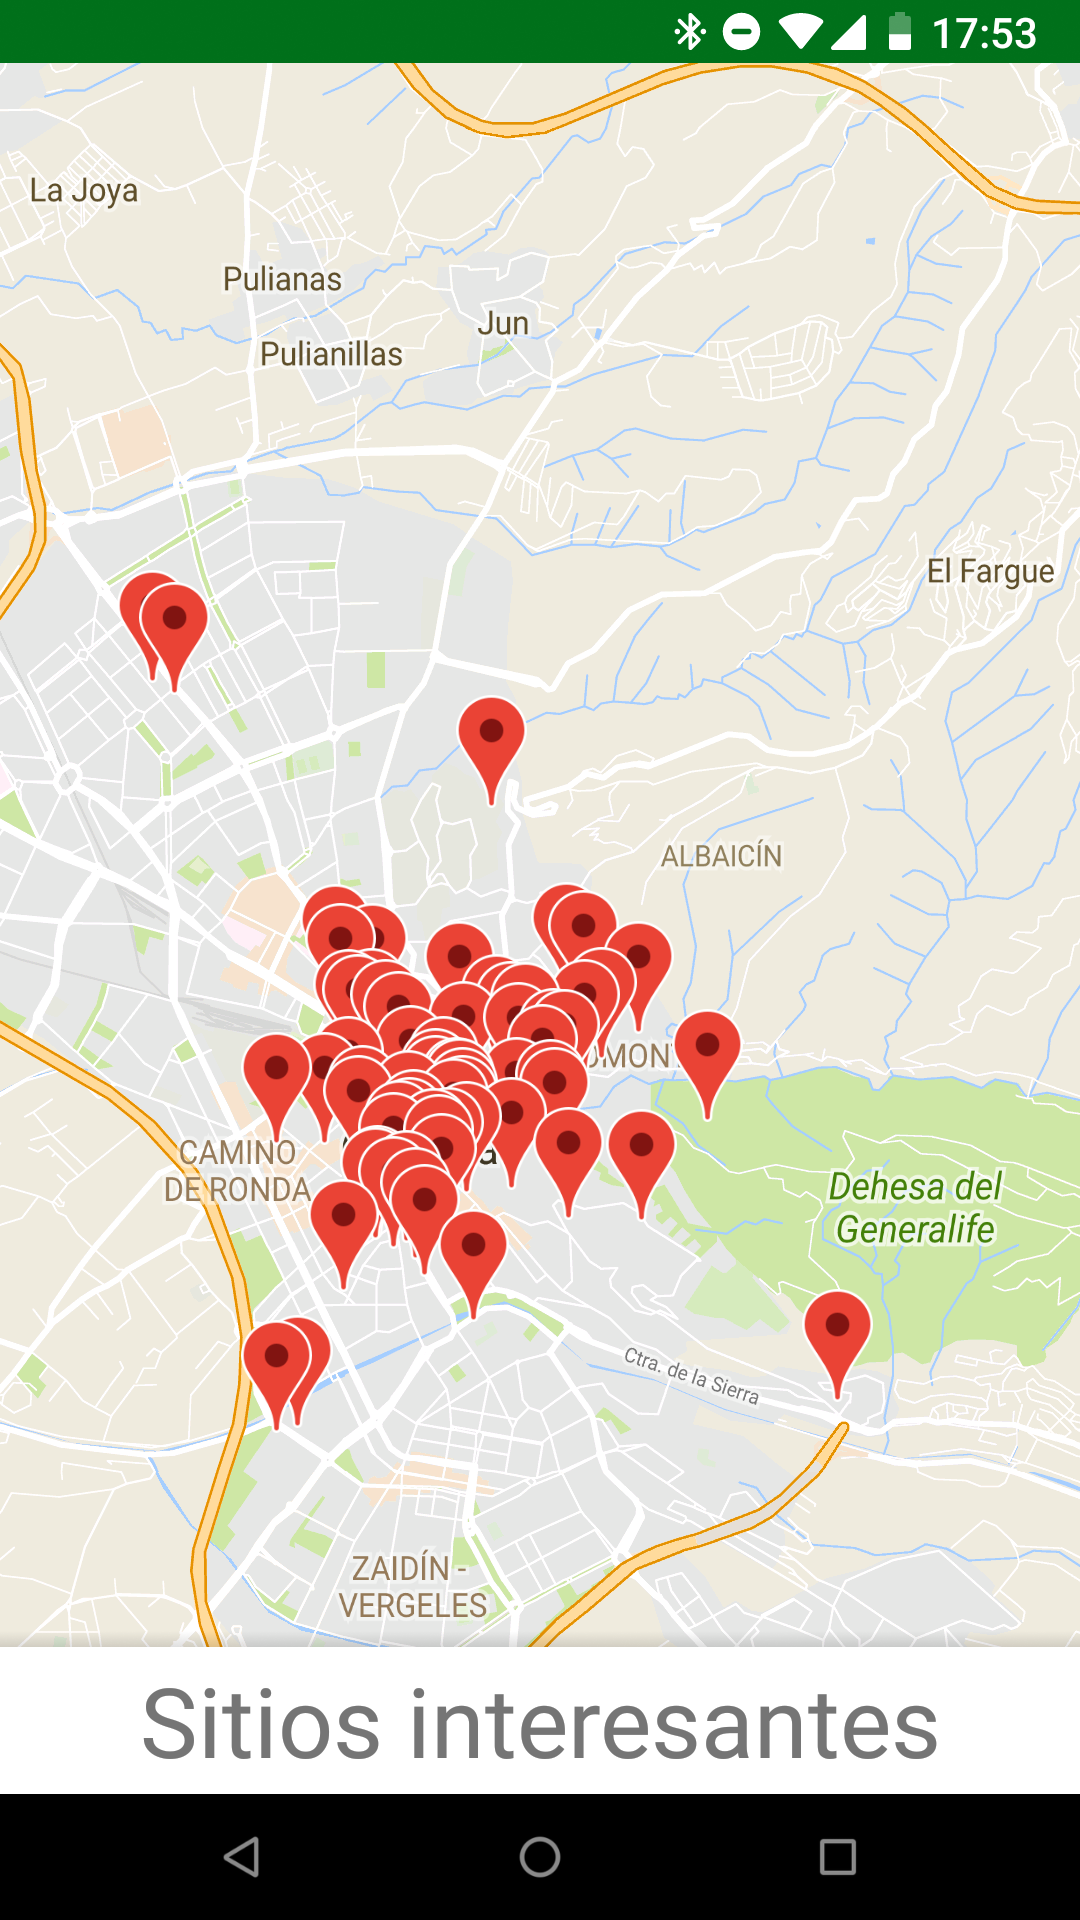
\includegraphics[width=50mm]{imagenes/main_activity_map}
	\caption{Mapa mostrando los puntos de interés y alojamientos sobre el mapa}
	\label{fig:main_activity_map}
\end{figure}
\vspace{0.06in}
\begin{figure}[H]
	\centering
	\subfigure{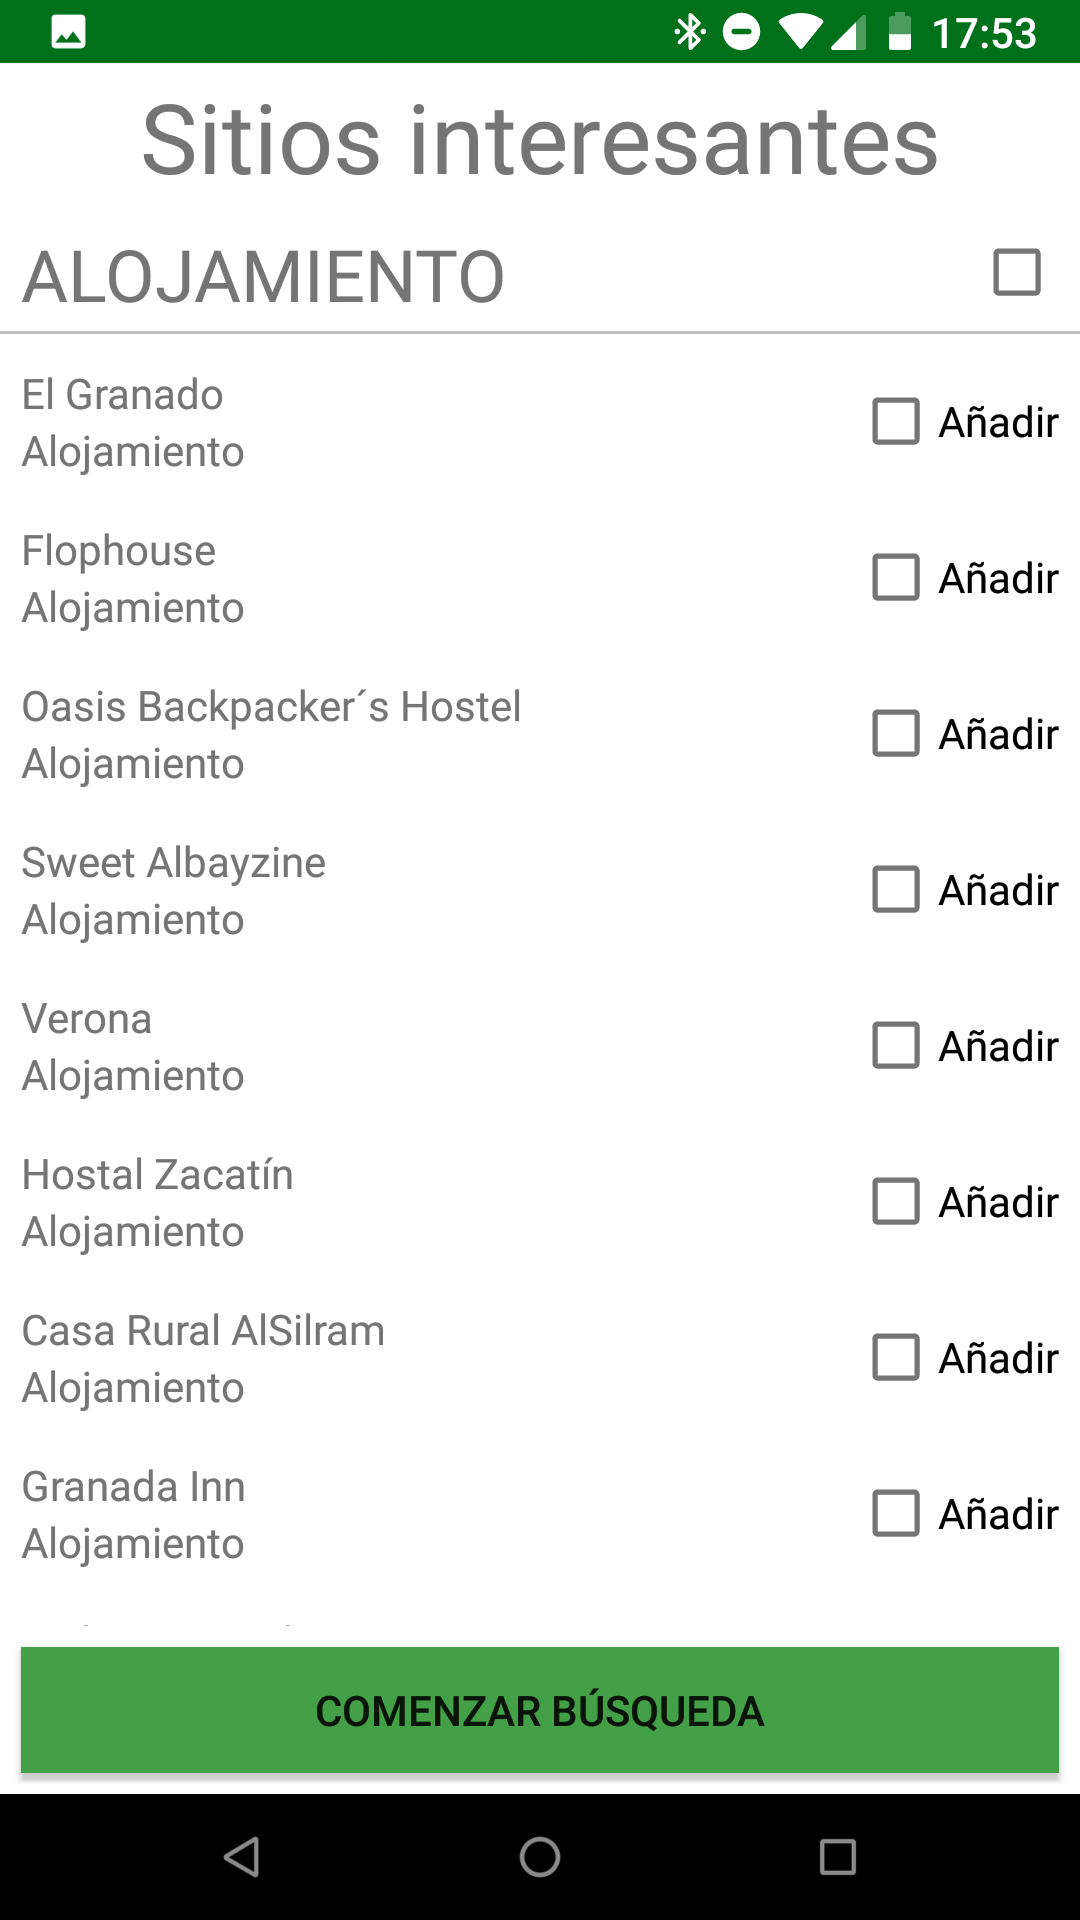
\includegraphics[width=50mm]{imagenes/main_activity_list}}
	\subfigure{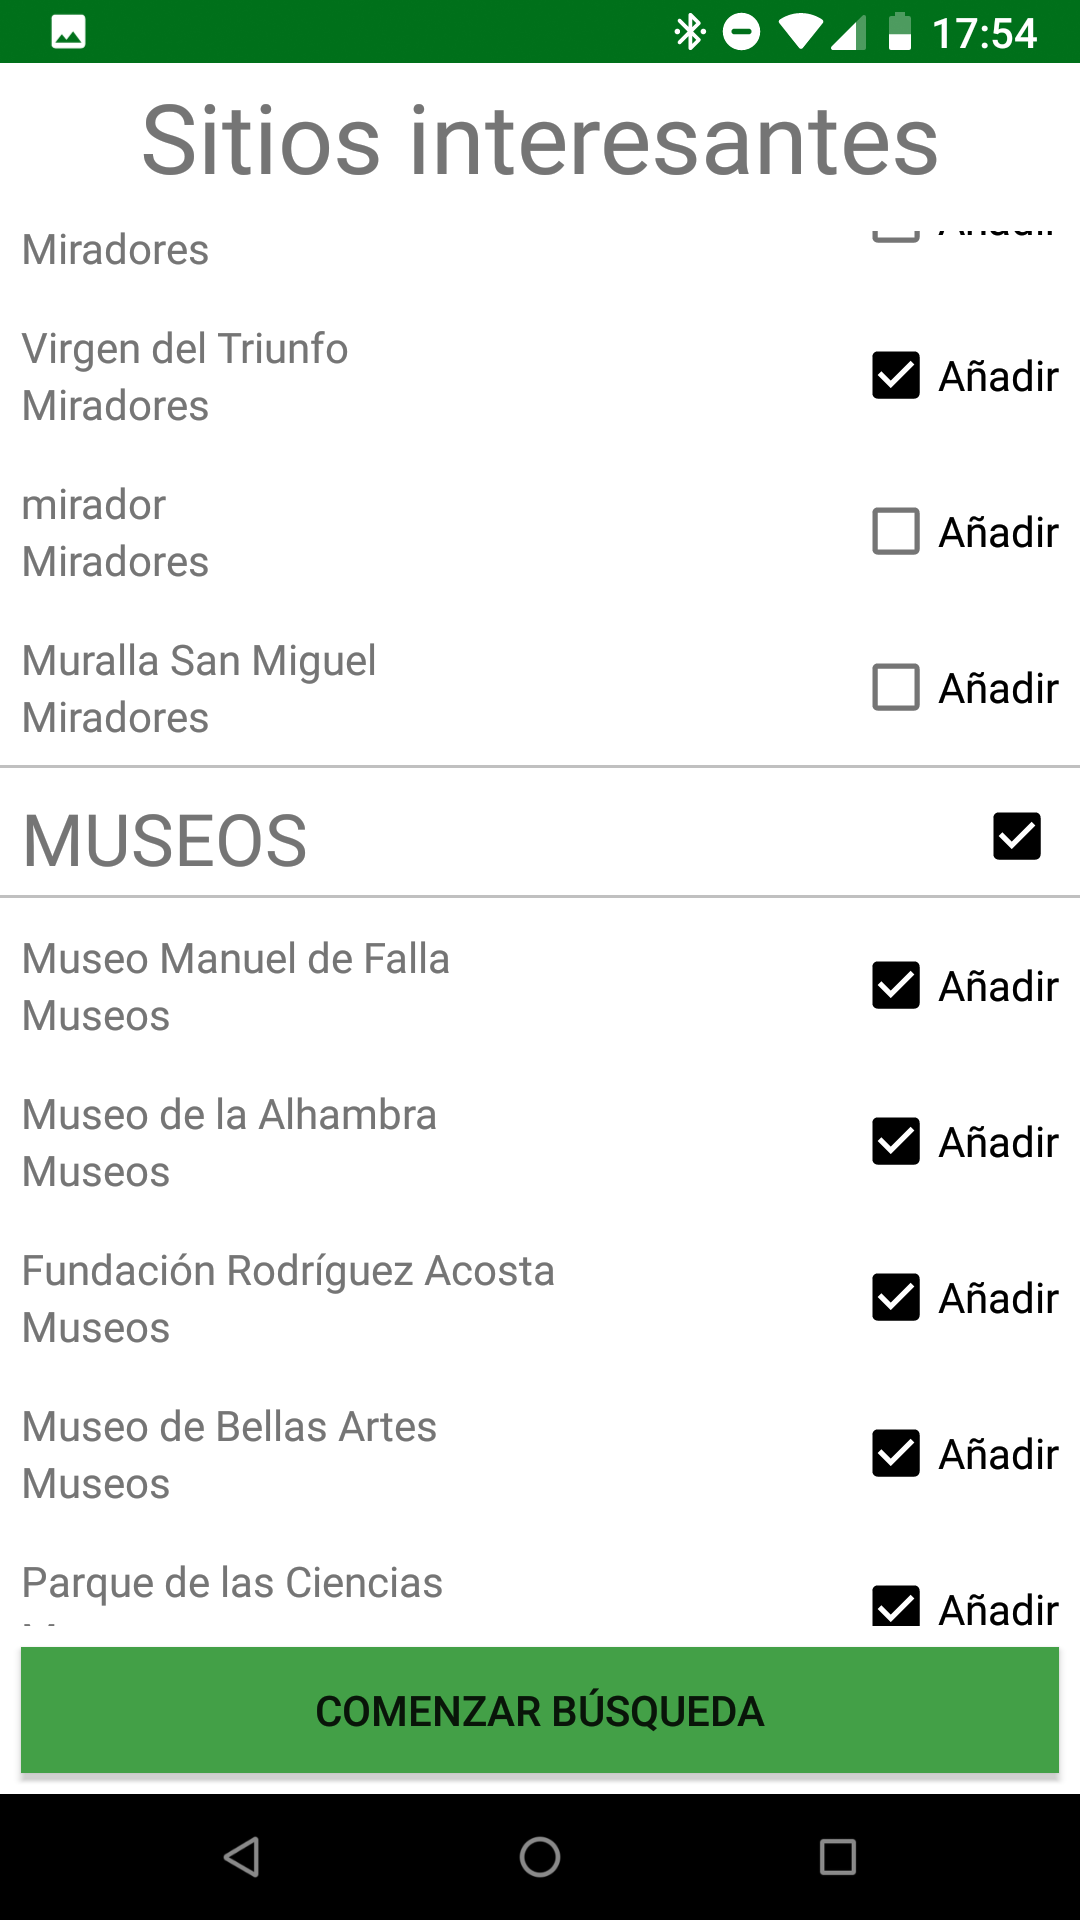
\includegraphics[width=50mm]{imagenes/main_activity_list_2}}
	\caption{Lista de alojamientos y puntos de interés disponibles para seleccionar}
	\label{fig:main_activity_list}
\end{figure}

\vspace{0.06in}
\begin{figure}
	\centering
	\subfigure{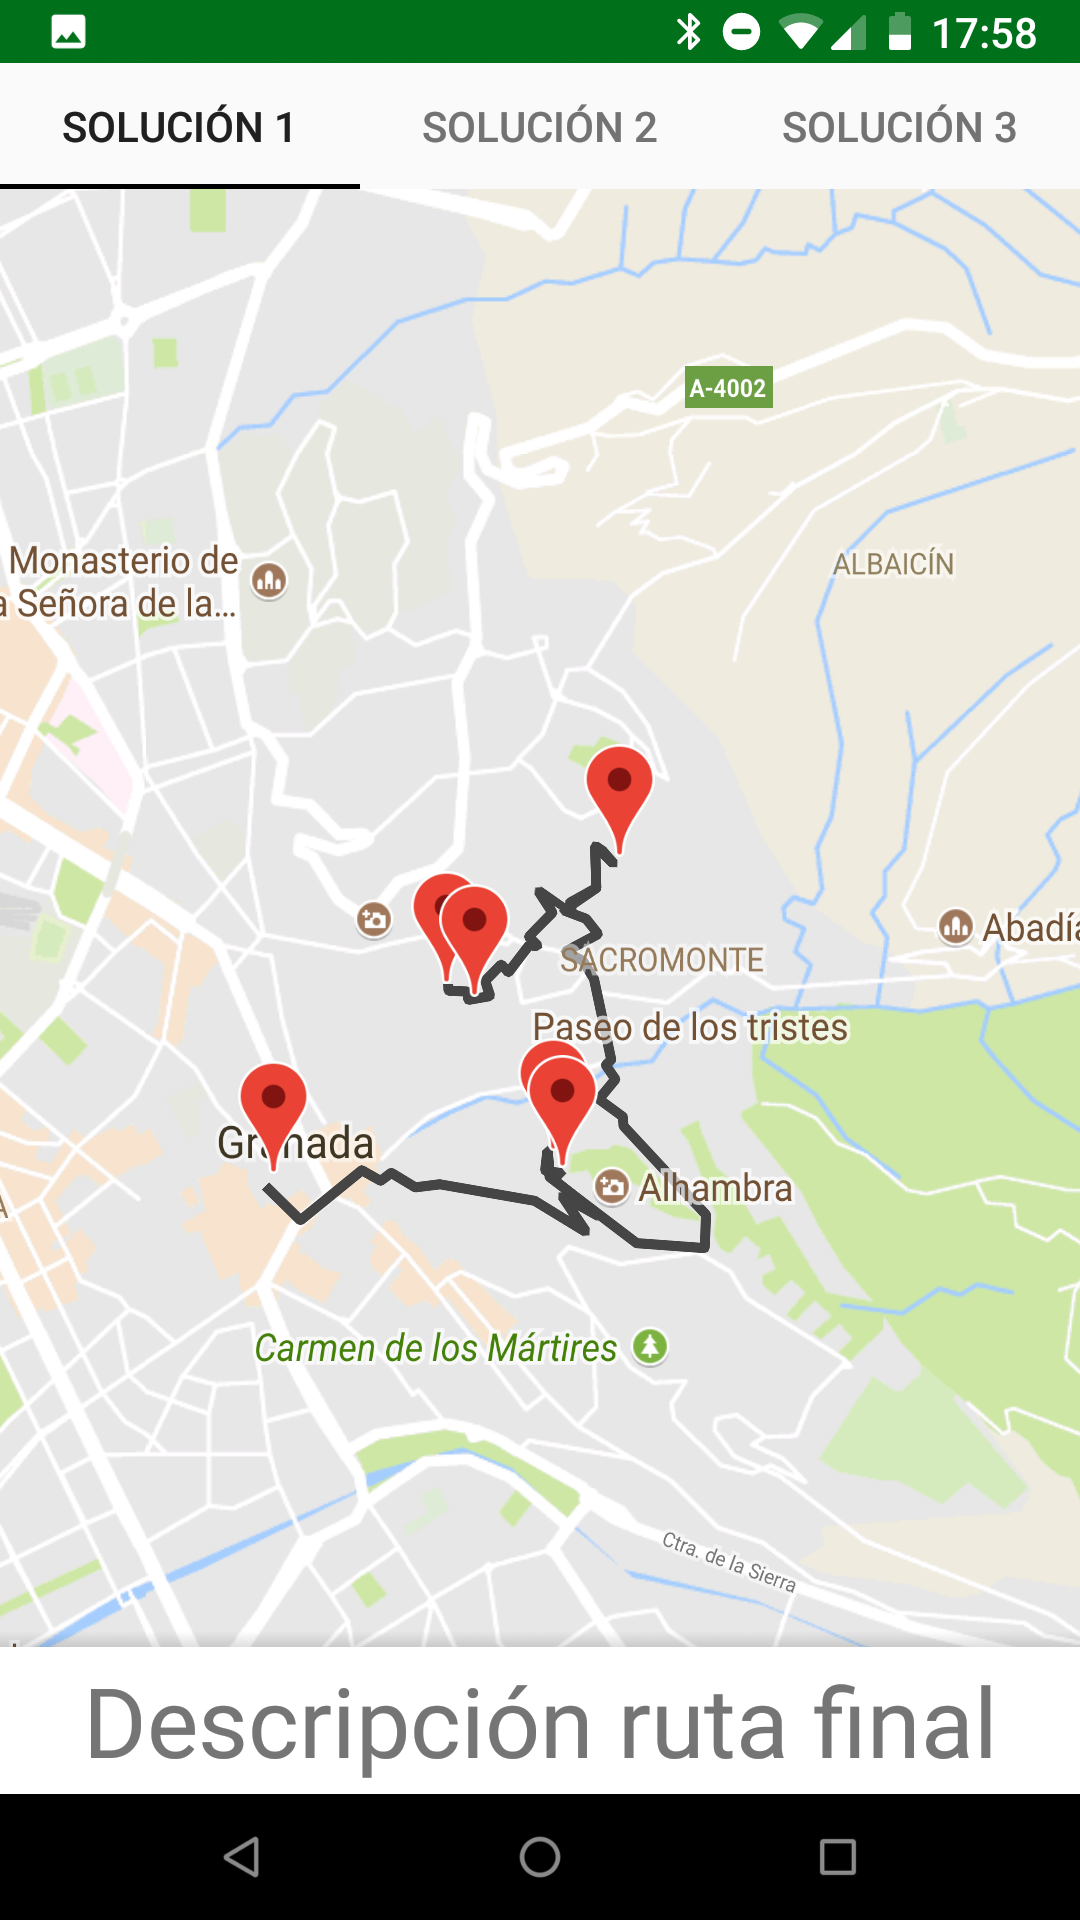
\includegraphics[width=50mm]{imagenes/solution}}
	\subfigure{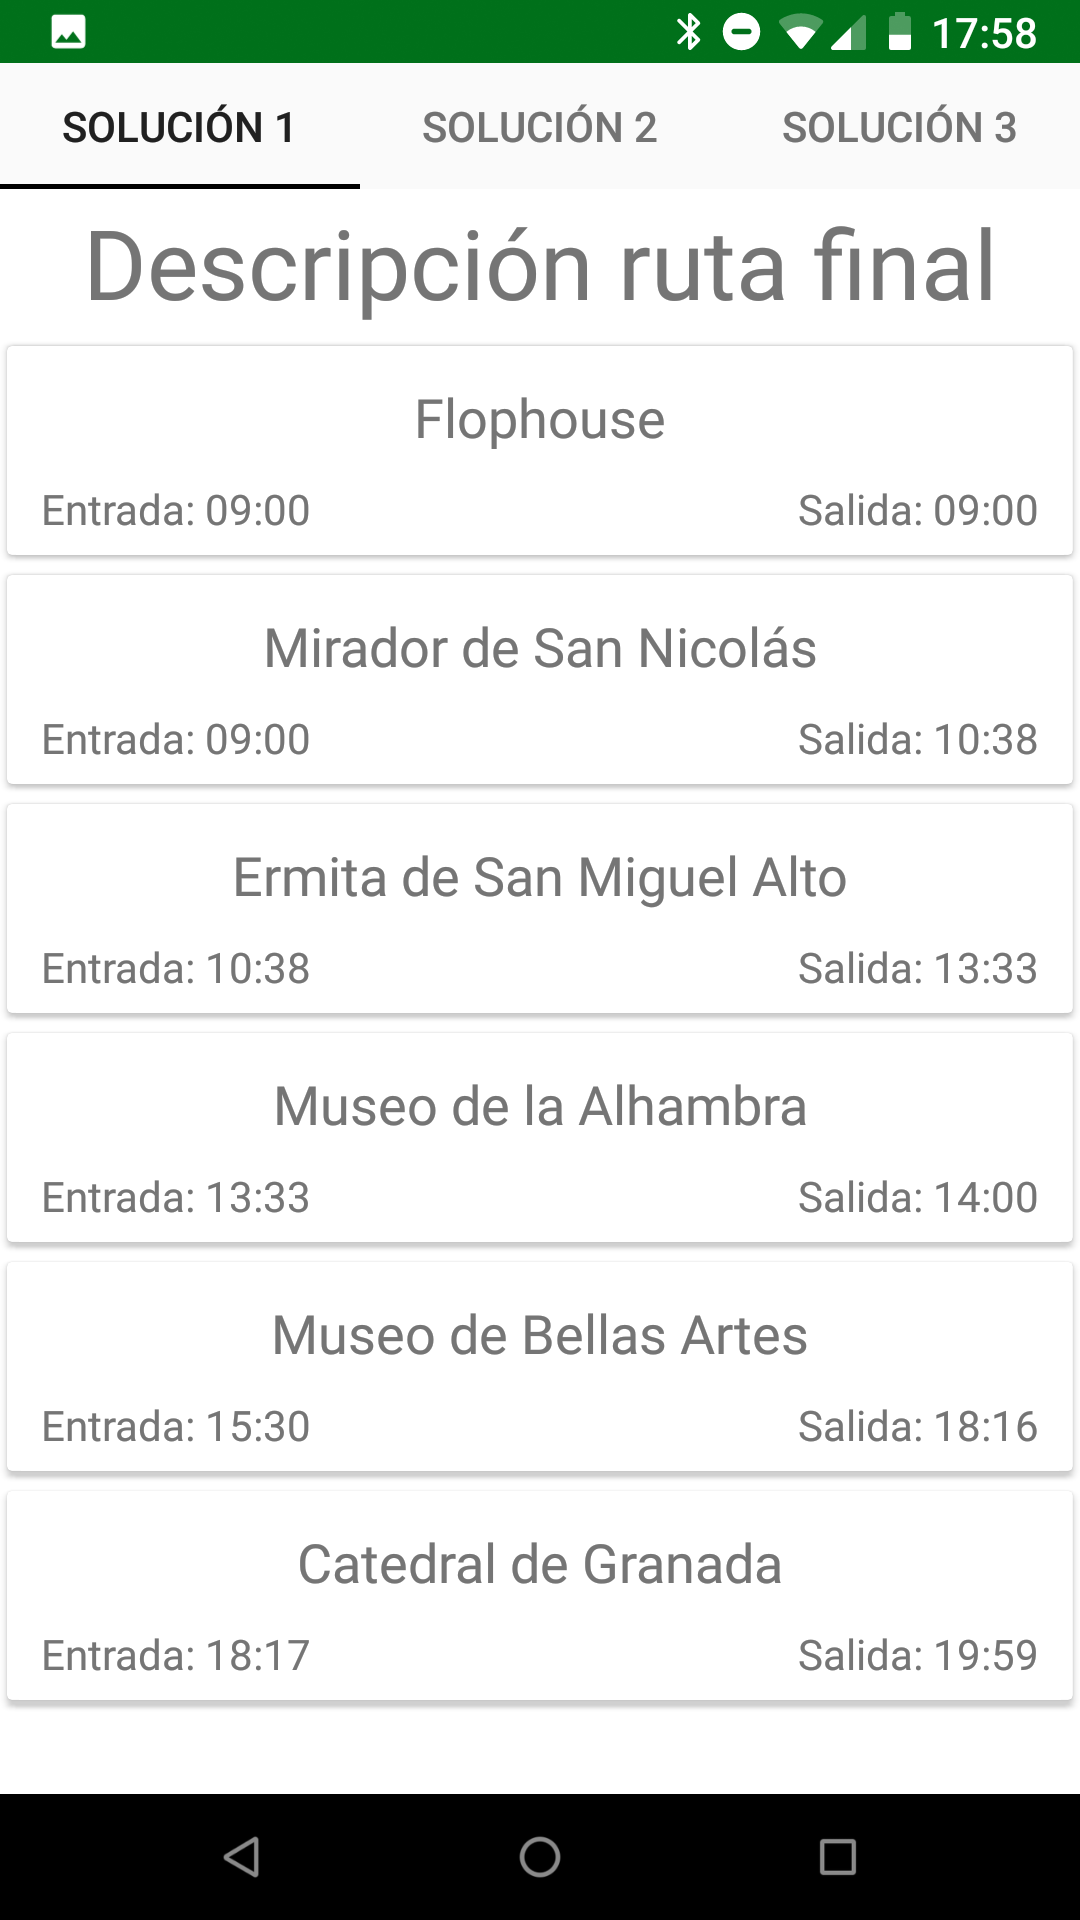
\includegraphics[width=50mm]{imagenes/list_solution}}
	\caption{Mapa mostrando solución y lista de puntos de interés de la solución}
	\label{fig:result_activity}
\end{figure}

\begin{figure}[H]
	\centering
	\subfigure{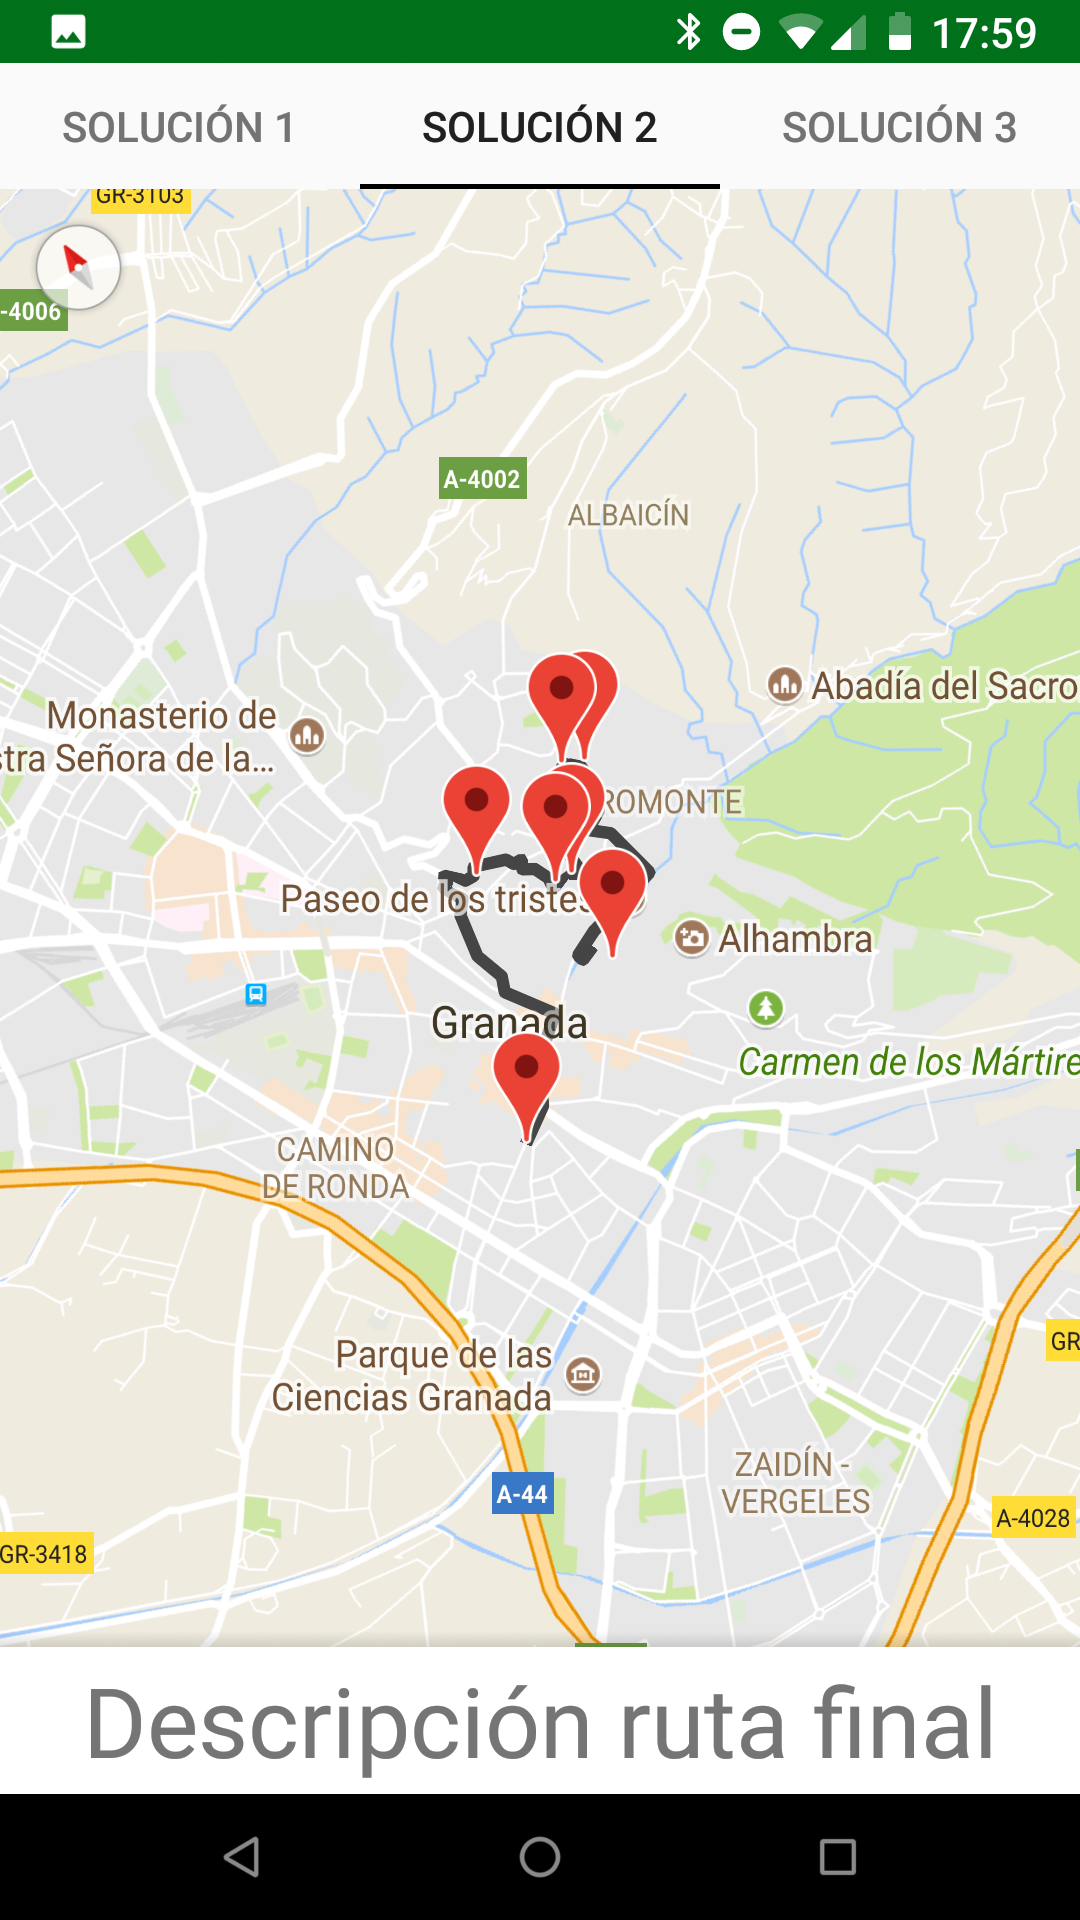
\includegraphics[width=50mm]{imagenes/solution_2}}
	\subfigure{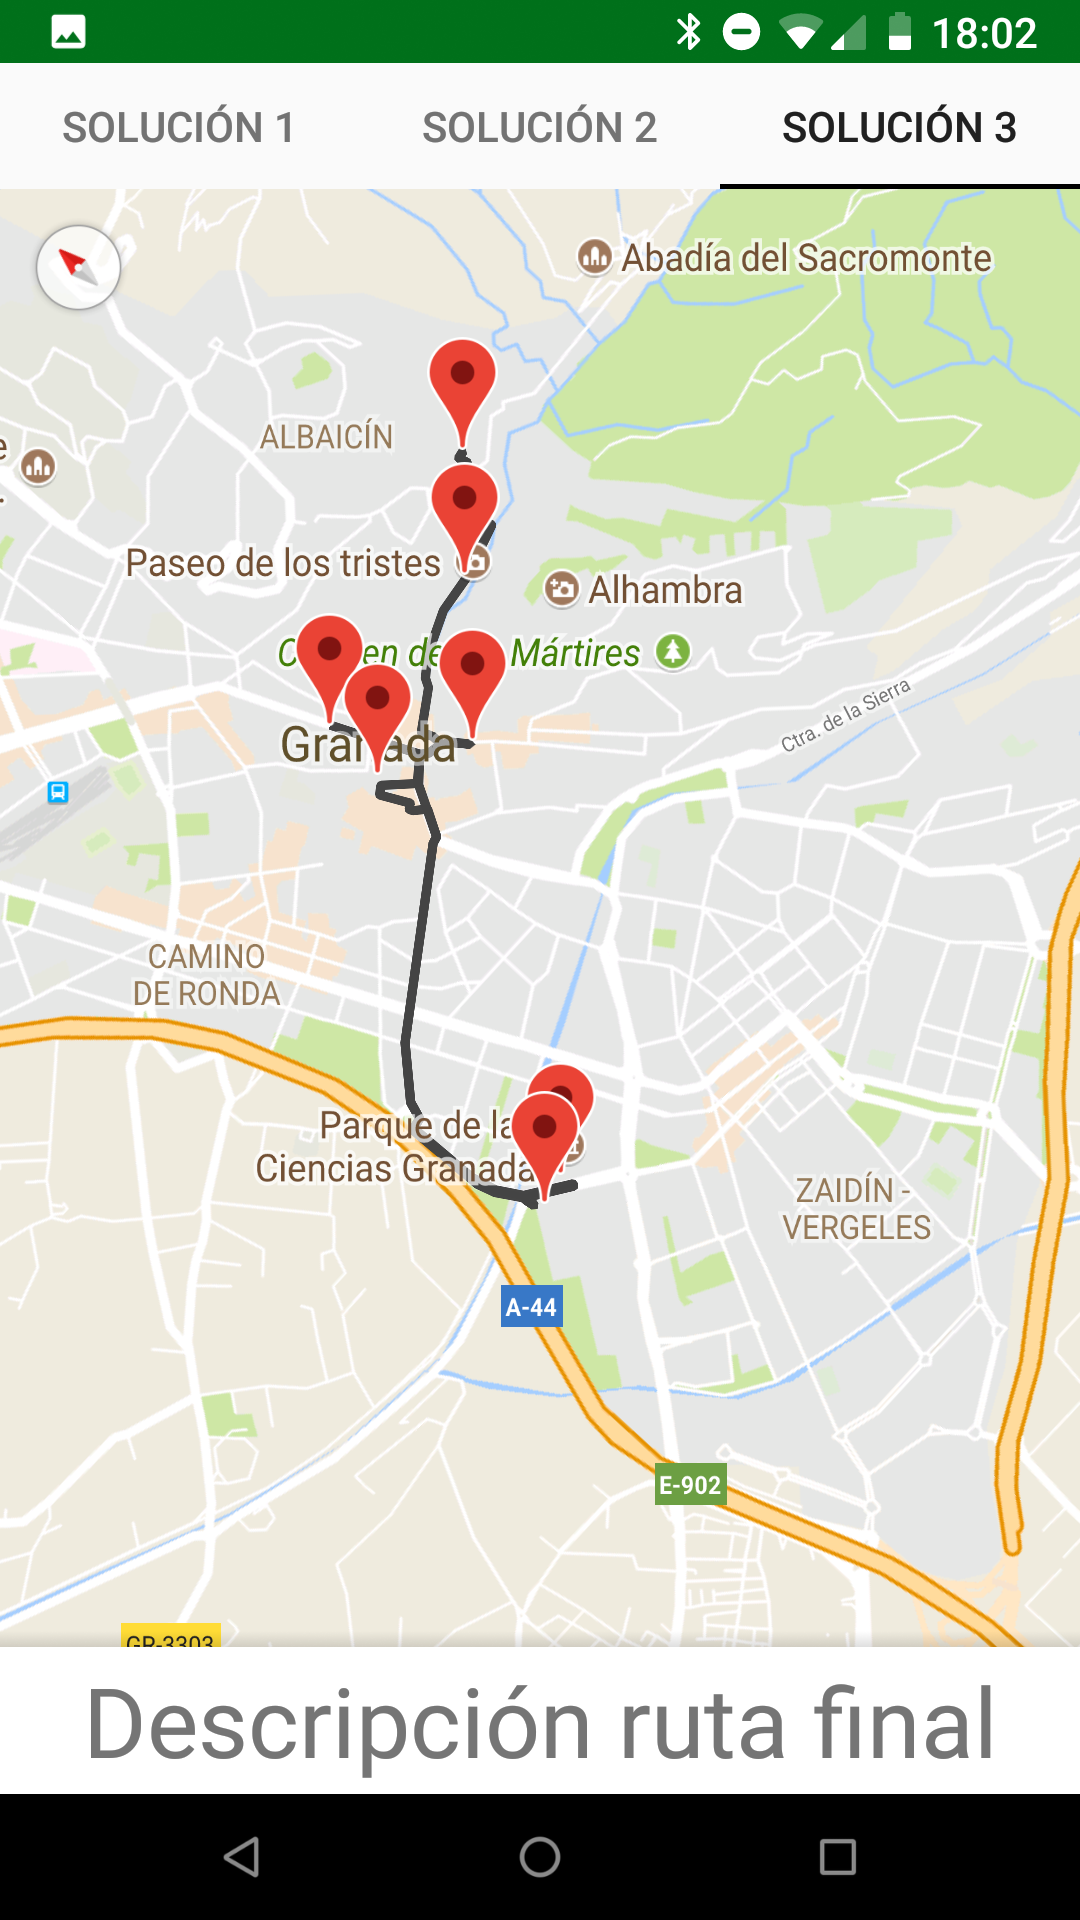
\includegraphics[width=50mm]{imagenes/solution_3}}
	\caption{Diferentes soluciones mostradas en un mapa}
	\label{fig:result_activity_2}
\end{figure}

%
%\chapter{Implementación}

En este apartado se mostrarán los aspectos más importantes del desarrollo del código de la aplicación, tanto en el lado de la interfaz como los procesos internos. Los métodos se organizarán en relación a los requisitos especificados en el análisis.

Todo el código de la aplicación está desarrollado en Java para Android.

\section[Interfaz de usuario]{Interfaz de usuario}
\subsection{Mostrar mapa}
Para mostrar el mapa se ha utilizado la vista que tiene integrada Android, para ello se debe crear una clave que  permita a la aplicación acceder a los servicios de Google Maps. Para ello, hay que crear al menos un plan estándar desde la página de Google Maps API. Una vez se tenga la clave, hay que crear una vista del mapa dentro de la actividad donde se quiera mostrar dicho mapa y implementar la interfaz OnMapReadyCallback, para la cual hay que implementar el método onMapReady(GoogleMap googleMap), el cuál se llama cuando se inicializa un objeto de la clase GoogleMaps y está preparado para usarse dentro de Android. El código necesario para mostrar el mapa es el siguiente.
\begin{lstlisting}[caption=código necesario para mostrar el mapa en la aplicación]
public class MapsActivity extends FragmentActivity implements OnMapReadyCallback, CustomClickListener {
	private GoogleMap mMap;
	...
	@Override
	protected void onCreate(Bundle savedInstanceState) {
		super.onCreate(savedInstanceState);
		
		/*
		* Inicializar otras vistas de la actividad
		*/
		
		// Obtain the SupportMapFragment and get notified when the map is ready to be used.
		SupportMapFragment mapFragment = (SupportMapFragment) getSupportFragmentManager()
		.findFragmentById(R.id.map);
		mapFragment.getMapAsync(this);
		initFragment();
		
		Log.e("map: ", "mapa puesto");
	}
	
	/*
	* Otros procesos de la actividad
	*/
	
	@Override
	public void onMapReady(GoogleMap googleMap) {
	mMap = googleMap;
		try {
		// Customise the styling of the base map using a JSON object defined
		// in a raw resource file.
		boolean success = googleMap.setMapStyle(
			MapStyleOptions.loadRawResourceStyle(
			this, R.raw.style_json));
		
		if (!success) {
			Log.e("map_style", "Style parsing failed.");
		}
		} catch (Resources.NotFoundException e) {
			Log.e("map_style", "Can't find style. Error: ", e);
		}
		
		
		
		// Add a marker in Sydney and move the camera
		LatLng granada = new LatLng(lat_granada, lon_granada );
		mMap.moveCamera(CameraUpdateFactory.newLatLngZoom(granada,13));
	}
}
\end{lstlisting}
El archivo de la vista de la actividad sería el siguiente.
\begin{lstlisting}[caption=Código XML de la vista de la actividad principal]
<android.support.constraint.ConstraintLayout xmlns:android="http://schemas.android.com/apk/res/android"
	xmlns:tools="http://schemas.android.com/tools"
	android:layout_width="match_parent"
	android:layout_height="match_parent">

	<com.sothree.slidinguppanel.SlidingUpPanelLayout xmlns:sothree="http://schemas.android.com/apk/res-auto"
	android:id="@+id/sliding_panel"
	android:layout_width="match_parent"
	android:layout_height="match_parent"
	android:gravity="bottom"
	sothree:layout_constraintBottom_toBottomOf="parent"
	sothree:layout_constraintEnd_toEndOf="parent"
	sothree:layout_constraintStart_toStartOf="parent"
	sothree:layout_constraintTop_toTopOf="parent"
	sothree:umanoDragView="@id/recyclerLayout"
	sothree:umanoOverlay="true"
	sothree:umanoPanelHeight="?android:attr/actionBarSize"
	sothree:umanoShadowHeight="6dp">

		<!-- MAIN CONTENT -->
		<fragment
		android:id="@+id/map"
		android:name="com.google.android.gms.maps.SupportMapFragment"
		android:layout_width="match_parent"
		android:layout_height="match_parent"
		/>
		
		<!-- SLIDING LAYOUT -->
		<FrameLayout
		android:id="@+id/recyclerLayout"
		android:layout_width="match_parent"
		android:layout_height="match_parent" />
	
	</com.sothree.slidinguppanel.SlidingUpPanelLayout>

</android.support.constraint.ConstraintLayout>
\end{lstlisting}
\subsection{Lista de puntos de interés/alojamiento y lista solución}
Para crear una lista en Android existen diferentes estructuras, la más reciente y más versátil es crear un RecyclerView. Para utilizar un RecyclerView en Android, se debe utilizar un objeto de la clase RecyclerView en la actividad o fragment en el que se vaya a mostrar la lista. Además, hay que crear una clase que herede de la clase RecyclerView.Adapter para indicar el comportamiento de la lista, dentro de esta clase se debe sobreescribir al menos los métodos onCreateViewHolder(), que es llamado cuando se crea un nuevo objeto en la lista; onBindViewHolder(), que es llamado cuando se va a mostrar un objeto en pantalla de la lista y se le asocia una posición dentro de la lista; y la función getItemCount(), que devuelve el número de elementos de la lista.\newline

Una vez se haya creado este objeto se debe de indicar al RecyclerView cual es el Adapter que se va a utilzar, esto se hace con el método RecyclerView.SetAdapter(Clase\_Adapter). También es necesario especificar el layout que tendrá el RecyclerView, para ello hay que utilizar el método RecyclerView.setLayoutManager(tipo\_layout\_manager); existen diferentes tipos de layout posibles para el RecyclerView, pero si se quiere mostrar una lista se debe utilizar como \enquote{tipo\_layout\_manager} un objeto de la clase LinearLayoutManager; para este objeto hay que especificar el contexto al crear el objeto, para ello se debe utilizar la función getActivity(), si se va a utilizar dentro de un Fragment, o this si se va a utilizar en una Activity.El código necesario para esto sería el siguiente.

\begin{lstlisting}[caption=Código de una clase que contiene un RecyclerView]
public class TypesFragment extends Fragment {

	private RecyclerView mRecycler;
	private TypesRecyclerAdapter mAdapter;
	private Button searchButton;
	private ArrayList<?extends ModelNode> mList = new ArrayList<>();
	private String TAG = TypesFragment.class.getSimpleName();
	private CustomClickListener listener;
	
	public TypesFragment() {
	// Required empty public constructor
	}
	
	...
	
	@Override
	public void onCreate(Bundle savedInstanceState) {
		super.onCreate(savedInstanceState);
	}
	
	@Override
	public View onCreateView(LayoutInflater inflater, ViewGroup container,
	Bundle savedInstanceState) {
	
	// Init recyclerView
	View recyclerViewLayout = inflater.inflate(R.layout.fragment_types, container, false);
	searchButton = (Button) recyclerViewLayout.findViewById(R.id.busqueda);
	mRecycler = (RecyclerView) recyclerViewLayout.findViewById(R.id.recycler);
	mAdapter = new TypesRecyclerAdapter(mList);
	mRecycler.setLayoutManager(new LinearLayoutManager(getActivity()));
	mRecycler.setAdapter(mAdapter);
	
	searchButton.setOnClickListener(new View.OnClickListener() {
			@Override
			public void onClick(View v) {
				listener.onSearchButtonClick(getSelected());
			}
		});
	
	return recyclerViewLayout;
	}
		
	...

}
\end{lstlisting}
 
\begin{lstlisting}[caption=Código para crear una lista en Android]
public class TypesRecyclerAdapter extends RecyclerView.Adapter<RecyclerView.ViewHolder> {

private String TAG = TypesRecyclerAdapter.class.getSimpleName();
private ArrayList<?extends ModelNode> tipos = new ArrayList<>();
private HashMap<String, Vector<String>> selected = new HashMap<>();
private ArrayList<String> type_selected = new ArrayList<>();

public TypesRecyclerAdapter(ArrayList< ?extends ModelNode> all) {
	this.tipos = all;
}

public void setTipos(ArrayList<?extends ModelNode> tipos){
	this.tipos = tipos;
}

@Override
public int getItemViewType(int position) {
	int pos=0;
	if(tipos.get(position).getClass().toString().contains("CityNode")){
		pos = 2;
	}
	return pos;
}

@Override
public RecyclerView.ViewHolder onCreateViewHolder(ViewGroup parent, int viewType) {
	View view;
	switch (viewType){
		case 0:
			view = LayoutInflater.from(parent.getContext()).inflate(R.layout.types_viewholder,
			parent, false);
			return new TypeViewHolder(view);
		
		case 2:
			view = LayoutInflater.from(parent.getContext()).inflate(R.layout.nodes_viewholder,
			parent,false);
			return new CityNodesViewHolder(view);
	}
	return null;
}

@Override
public void onBindViewHolder(final RecyclerView.ViewHolder holder, final int position) {
	switch (holder.getItemViewType()){
	case 0:
		final TypeViewHolder typeViewHolder = (TypeViewHolder) holder;
		final TypeOfNode typeNode = (TypeOfNode) tipos.get(position);
		typeViewHolder.setTypeText(typeNode.getName());
		typeViewHolder.setCheck(isInTypeSelected(typeNode.getName()));
		typeViewHolder.setOnClickListener(new View.OnClickListener(){
			@Override
			public void onClick(View v){
				typeViewHolder.changeChecked();
				addOrRemoveType(typeNode.getName());
			}
			});
		break;
	case 2:
		final CityNode cityNode = (CityNode) tipos.get(position);
		final CityNodesViewHolder node = (CityNodesViewHolder) holder;
		node.setNodeName(cityNode.getName());
		node.setNodeType(cityNode.getType());
		node.setCheck(isInSelected(cityNode.getType(),cityNode.getName()));
		node.setOnClickListener(new View.OnClickListener() {
		@Override
			public void onClick(View v) {
				node.changeChecked();
				addOrRemoveNode(cityNode.getType(), cityNode.getName());
			}
			});
	break;
}


}

...


@Override
public int getItemCount() {
	return tipos.size();
}
\end{lstlisting}

\begin{lstlisting}[caption=Código XML de la vista de una lista de elementos]
<?xml version="1.0" encoding="utf-8"?>
<android.support.constraint.ConstraintLayout xmlns:android="http://schemas.android.com/apk/res/android"
	xmlns:app="http://schemas.android.com/apk/res-auto"
	xmlns:tools="http://schemas.android.com/tools"
	android:id="@+id/typesLayout"
	android:layout_width="match_parent"
	android:layout_height="match_parent"
	tools:context=".fragment.TypesFragment"
	android:background="@color/white"
	>


	<android.support.v7.widget.RecyclerView
	android:id="@+id/recycler"
	android:layout_width="0dp"
	android:layout_height="0dp"
	android:layout_marginBottom="8dp"
	android:layout_marginTop="8dp"
	android:clickable="true"
	android:focusable="true"
	app:layout_constraintBottom_toTopOf="@+id/busqueda"
	app:layout_constraintEnd_toEndOf="parent"
	app:layout_constraintStart_toStartOf="parent"
	app:layout_constraintTop_toBottomOf="@+id/textView"
	tools:listitem="@layout/types_viewholder" />
	
	<TextView
	android:id="@+id/textView"
	android:layout_width="0dp"
	android:layout_height="?android:attr/actionBarSize"
	android:layout_marginEnd="8dp"
	android:layout_marginStart="8dp"
	android:text="@string/textViewSlideUpPanel"
	android:textSize="32sp"
	app:layout_constraintEnd_toEndOf="parent"
	app:layout_constraintHorizontal_bias="1.0"
	app:layout_constraintStart_toStartOf="parent"
	app:layout_constraintTop_toTopOf="parent"
	android:gravity="center"/>
	
	<Button
	android:id="@+id/busqueda"
	android:layout_width="0dp"
	android:layout_height="wrap_content"
	android:layout_marginBottom="8dp"
	android:layout_marginEnd="8dp"
	android:layout_marginStart="8dp"
	android:background="@color/searchGreen"
	android:text="@string/startSearch"
	app:layout_constraintBottom_toBottomOf="parent"
	app:layout_constraintEnd_toEndOf="parent"
	app:layout_constraintStart_toStartOf="parent" />
</android.support.constraint.ConstraintLayout>
\end{lstlisting}

Una vez se tiene  creada y definida la lista, se debe crear una clase más para especificar la vista y el comportamiento individual de cada uno de los elementos de dicha lista. Esta nueva clase debe heredar de la clase RecyclerView.ViewHolder; esta debe tener además un fichero XML que defina la estructura de la vista de dicha clase. El código necesario para crear dicha clase es el siguiente.

\begin{lstlisting}[caption=Código para crear un elemento de una lista en Android]
public class CityNodesViewHolder extends RecyclerView.ViewHolder {
	private TextView nodeName;
	private TextView nodeType;
	private CheckBox mAddButton;
	private String TAG = CityNodesViewHolder.class.getSimpleName();
	private boolean isChecked = false;
	
	public CityNodesViewHolder(View itemView){
		super(itemView);
		nodeName = (TextView) itemView.findViewById(R.id.nodeName);
		mAddButton = (CheckBox) itemView.findViewById(R.id.addButton);
		nodeType = (TextView) itemView.findViewById(R.id.type_name);
		mAddButton.setChecked(isChecked);
	}
	...
}
\end{lstlisting}

\begin{lstlisting}[caption=Código XML de la vista de un elemento de la lista]
<?xml version="1.0" encoding="utf-8"?>
<android.support.constraint.ConstraintLayout xmlns:android="http://schemas.android.com/apk/res/android"
	xmlns:app="http://schemas.android.com/apk/res-auto"
	xmlns:tools="http://schemas.android.com/tools"
	android:id="@+id/node_layout"
	android:layout_width="match_parent"
	android:layout_height="wrap_content">

	<TextView
	android:id="@+id/nodeName"
	android:layout_width="0dp"
	android:layout_height="wrap_content"
	android:layout_marginEnd="8dp"
	android:layout_marginStart="8dp"
	android:layout_marginTop="8dp"
	app:layout_constraintEnd_toStartOf="@+id/addButton"
	app:layout_constraintStart_toStartOf="parent"
	app:layout_constraintTop_toTopOf="parent" />
	
	<CheckBox
	android:id="@+id/addButton"
	android:layout_width="wrap_content"
	android:layout_height="wrap_content"
	android:layout_marginBottom="8dp"
	android:layout_marginEnd="8dp"
	android:layout_marginTop="8dp"
	android:text="@string/add_checkbox"
	app:layout_constraintBottom_toBottomOf="parent"
	app:layout_constraintEnd_toEndOf="parent"
	app:layout_constraintTop_toTopOf="parent" />
	
	<TextView
	android:id="@+id/type_name"
	android:layout_width="wrap_content"
	android:layout_height="wrap_content"
	android:layout_marginBottom="8dp"
	android:layout_marginStart="8dp"
	app:layout_constraintBottom_toBottomOf="parent"
	app:layout_constraintStart_toStartOf="parent"
	app:layout_constraintTop_toBottomOf="@+id/nodeName" />

</android.support.constraint.ConstraintLayout>
\end{lstlisting}

\subsection{Mostrar diferentes soluciones}
Para mostrar diferentes soluciones se optó por mostrar cada una de las diferentes soluciones en un mapa distinto, para ello, se debe crear una vista del mapa y una lista para mostrar la solución por cada solución; este proceso está explicado en los apartados anteriores, por lo que no se va a entrar en más detalle en este. Para poder navegar por las diferentes vistas de las soluciones, hay que crear una vista que permita seleccionar la vista de la solución que se quiera en cada momento, para esto se puede utilizar la clase TabLayout; dicha clase debe ir acompañada de un objeto de la clase ViewPager.\newline

La clase TabLayout solo se utiliza para definir tabs  que se muestran en pantalla, y cada uno de ellos hace referencia a una vista diferente. Para añadir comportamiento a cada uno de los tabs, se debe preparar al TabLayout para ser usado por la clase ViewPager, esto se hace utilizando el método TabLayout.setupWithViewPager(viewpager\_obj).\newline

Para definir el comportamiento del objeto de la clase ViewPager, hay que crear una clase que defina dicho comportamiento y especificárselo al objeto de la clase ViewPager con el método ViewPager.setAdapter(adapter). Una de las posibles formas de hacer esto es crear una clase interna a la clase en la que se utiliza el ViewPager que herede de la clase FragmentViewPager. Dentro de esta clase se deben sobreescribir al menos los métodos getItem(), que determina el Frament que se debe utilizar para cada tab; getCount(), que devuelve el número de tabs; y getPageTitle(), que determina el nombre de cada uno de los tabs según su posición. \newline

El siguiente código se encarga de hacer lo descrito en los párrafos anteriores.
\begin{lstlisting}[caption=Código de una vista con tabs dentro de ella]
public class ResultActivity extends FragmentActivity  {

	/*
	* Atributos de la clase
	*/
	
	
	@Override
	protected void onCreate(Bundle savedInstanceState) {
		super.onCreate(savedInstanceState);
		/*
		* Inicializar de otras vistas y atributos
		*/
		
		ViewPager viewPager = (ViewPager) findViewById(R.id.viewpager);
		SimpleFragmentPagerAdapter adapter = new SimpleFragmentPagerAdapter(this, getSupportFragmentManager());
		viewPager.setAdapter(adapter);
		
		TabLayout tabLayout = (TabLayout) findViewById(R.id.sliding_tabs);
		tabLayout.setupWithViewPager(viewPager);
	}
	
	public class SimpleFragmentPagerAdapter extends FragmentPagerAdapter {
	
		private Context mContext;
		private String TAG = SimpleFragmentPagerAdapter.class.getSimpleName();
		
		public SimpleFragmentPagerAdapter(Context context, FragmentManager fm) {
			super(fm);
			mContext = context;
		}
		
		// This determines the fragment for each tab
		@Override
		public Fragment getItem(int position) {
			Log.i(TAG,"position "+ position);
			if (position == 0) {
				return SolutionFragment.newInstance(entradas,salidas,identificadores,lat_ids,lon_ids,lat_city,lon_city);
			} else if (position == 1){
				return SolutionFragment.newInstance(entradas,salidas,identificadores,lat_ids,lon_ids,lat_city,lon_city);
			} else if (position == 2){
				return SolutionFragment.newInstance(entradas,salidas,identificadores,lat_ids,lon_ids,lat_city,lon_city);
			} else{
				return null;
			}
		}
		
		// This determines the number of tabs
		@Override
		public int getCount() {
			return 3;
		}
		
		// This determines the title for each tab
		@Override
		public CharSequence getPageTitle(int position) {
			// Generate title based on item position
			switch (position) {
			case 0:
				return "Sol 1";
			case 1:
				return "Sol 2";
			case 2:
				return "Sol 3";
			default:
				return null;
			}
		}
	}

}
\end{lstlisting}
\begin{lstlisting}[caption=Código XML de la vista con tabs]
<?xml version="1.0" encoding="utf-8"?>
<LinearLayout xmlns:android="http://schemas.android.com/apk/res/android"
	xmlns:app="http://schemas.android.com/apk/res-auto"
	android:id="@+id/result_constraint"
	android:layout_width="match_parent"
	android:layout_height="match_parent"
	android:orientation="vertical">

	<android.support.design.widget.TabLayout
	android:id="@+id/sliding_tabs"
	android:layout_width="match_parent"
	android:layout_height="wrap_content"
	app:tabMode="fixed" />
	
	<android.support.v4.view.ViewPager
	android:id="@+id/viewpager"
	android:layout_width="match_parent"
	android:layout_height="match_parent"
	android:background="@android:color/white" />

</LinearLayout>
\end{lstlisting}


\section[Procesos internos]{Procesos internos}
En este apartado se describirán las funciones de envío de peticiones a servidores, procesado de las respuestas de los servidores y el cálculo de la ruta óptima.
\subsection{Peticiones a servidores}
La aplicación cuenta con procesos que se encargan de mandar peticiones a servidores para obtener información sobre puntos de interés, distancias entre puntos, o camino óptimo entre dos puntos. Para enviar dichas peticiones, se debe especificar una URL para la cual el servidor pueda devolver una respuesta, una vez se ha obtenido la respuesta se guarda en un archivo o en un String para procesarlo. La función que descarga las respuestas de servidores se puede encontrar en la función doInBackground() de la clase DownloadFileFromURL.
\begin{lstlisting}[caption=Función para enviar peticiones a servidores y guardar respuesta]
@Override
protected String doInBackground(String... f_url) {
	int count;
	// Output stream
	String baseFolder = mContext.getFilesDir().getAbsolutePath();
	File file = new File(baseFolder + File.separator + f_url[1]);
	Log.i(TAG,"starting download");
	
	
	try {
		URL url = new URL(f_url[0]);
		HttpURLConnection conection = (HttpURLConnection) url.openConnection();
		
		// download the file
		InputStream input = new BufferedInputStream(url.openStream(),
		8192);
		
		file.getParentFile().mkdirs();
		OutputStream output = new FileOutputStream(file);
		
		Log.i(TAG,"file_out: "+"File opened");
		Log.i(TAG,"file_out:"+ "File saved in: " + mContext.getFilesDir().getAbsolutePath());
		
		byte data[] = new byte[1024];
		
		long total = 0;
		
		while ((count = input.read(data)) != -1) {
		total += count;
		
		// writing data to file
		output.write(data, 0, count);
		}
		
		// flushing output
		output.flush();
		
		// closing streams
		output.close();
		input.close();
		
		conection.disconnect();
		
		Log.i(TAG,"file_out:"+ "Finished writting output");
	
	} catch (Exception e) {
		Log.e(TAG, e.getMessage());
	}
	
	return baseFolder + File.separator + f_url[1];
}
\end{lstlisting}

Cuando la función termina, devuelve el PATH donde está guardado el archivo que contiene la respuesta del servidor. El parámetro que se le pasa a la función doInBackground(String... f\_url) se trata de un vector que contiene como primer elemento la URL que la función debe abrir y guardar el contenido; el segundo elemento contiene el nombre del archivo que contendrá la respuesta del servidor.
\subsection{Procesado de respuestas de servidor}
Para el procesado de la información que devuelven los servidores, se ha creado la clase JsonParser. Esta clase procesa los archivos y guarda la información en estructuras para poder utilizarlas después. Para procesar los datos, se debe pasar el PATH del archivo, para abrirlo y meterlo en un String que después se utilizará para inicializar un objeto del tipo JSONObject; o se puede pasar el String que contiene el fichero directamente.
\subsubsection{Procesado de alojamientos y puntos de interés}
Para el procesado del archivo que contiene la información sobre alojamientos y puntos de interés existe el método processJSON(), este método no tiene parámetros, por lo que hay que crear el objeto de la clase JsonParser indicando el PATH del archivo.\newline

Dentro de este método se recorre el array llamado \enquote{elements}, por cada uno de los elementos del array se crea un objeto JSONObject y se obtiene la información sobre el identificador del nodo, latitud, longitud, nombre y tipo de nodo en un hashmap. El código es el siguiente.\newline
\begin{lstlisting}[caption=Función para procesar información sobre puntos de interés y alojamientos]
public void processJSON() throws JSONException{
	JSONArray elements = file_info.getJSONArray("elements");
	for(int i=0; i < elements.length(); i++){
	JSONObject node = elements.getJSONObject(i);
	
	// Obtenemos datos del archivo.
	String id = node.optString("id");
	String latitud = node.optString("lat");
	String longitud = node.optString("lon");
	JSONObject tags = node.getJSONObject("tags");
	String name = tags.optString("name", "desconocido");
	
	String tipo = tags.optString("tourism");
	if( tipo.equals("") ){
		tipo = tags.optString("amenity");
	}
	
	
	HashMap<String, String> aux_hashMap = new HashMap<>();
	// Utilizamos un hashMap auxiliar.
	if( !name.equals("desconocido")) {
		aux_hashMap.put("id", id);
		aux_hashMap.put("lat", latitud);
		aux_hashMap.put("lon", longitud);
		aux_hashMap.put("name", name);
		
		if(!city_nodes.containsKey(tipo)){
			// Metemos un nuevo nodo.
			System.out.println("nuevo tipo: " + tipo);
			Vector<HashMap<String,String>> v_aux = new Vector<>();
			v_aux.add(aux_hashMap);
			city_nodes.put(tipo, v_aux);
		
		}else{
			System.out.println("adding new map to "+ tipo);
			city_nodes.get(tipo).add(aux_hashMap);
		}
	}
	
	
	}

}
\end{lstlisting}
\subsubsection{Procesado de la matriz de tiempos}
Para el procesado de la matriz se creó el método processOSRMJSON(), dicho método necesita que antes se inicialice el objeto de la clase JsonParser para que funcione correctamente.
Este método procesa el array llamado \enquote{durations} donde va guardando en una matriz el tiempo necesario para llegar desde un punto a otro en segundos. El código de dicho método es el siguiente.
\begin{lstlisting}[caption=Función para procesar matriz de tiempos entre puntos]
public void processOSMRJSON() throws JSONException{

	JSONArray times = file_info.getJSONArray("durations");
	ArrayList<Integer> tim = new ArrayList<>();
	for(int i=0; i < times.length(); i++){
		JSONArray aux_t = times.getJSONArray(i);
		for(int j=0; j < aux_t.length(); j++){
			int dist_time = aux_t.getInt(j);
			Log.i(TAG,dist_time+"");
			tim.add(dist_time);
		}
	
	segs.add(tim);
	tim = new ArrayList<>();
	}

}
\end{lstlisting}
\subsubsection{Procesado de caminos entre puntos de la solución}
Para el procesado de caminos entre dos puntos se creó el método parseRoutes(String geo\_coord). Este método recorre el array llamado \enquote{steps}, dentro de este array se toma el String \enquote{points} que está contenido en el objeto \enquote{polyline}, después este String se debe decodificar \cite{decode_polyline}. Para entrar en el array \enquote{steps} se debe primero entrar en el array \enquote{routes} y dentro de este en \enquote{legs}.\newline

El array \enquote{routes} contiene todas las rutas posibles entre los puntos que se le indiquen; las rutas se dividen en etapas, que representan la ruta entre dos puntos; dichas etapas se representan con los arrays \enquote{legs}. Dentro de una etapa puede haber más de un paso a seguir, dichos pasos se representan con los arrays \enquote{steps}.\newline

El código de la función de procesado de rutas y de decodificar las polilíneas es el siguiente.
\begin{lstlisting}[caption=Función para procesar los caminos entre los puntos de una ruta]
public List<List<HashMap<String,String>>> parseRoutes(String geo_coord) throws JSONException{
	JSONObject object = new JSONObject(geo_coord);
	Log.i(TAG,object.toString());
	List<List<HashMap<String, String>>> routes = new ArrayList<>() ;
	JSONArray jRoutes;
	JSONArray jLegs;
	JSONArray jSteps;
	
	try {
	
		jRoutes = object.getJSONArray("routes");
		
		
		for(int i=0;i<jRoutes.length();i++){
			jLegs = ( (JSONObject)jRoutes.get(i)).getJSONArray("legs");
			List path = new ArrayList<>();
			
			for(int j=0;j<jLegs.length();j++){
				jSteps = ( (JSONObject)jLegs.get(j)).getJSONArray("steps");
				
				for(int k=0;k<jSteps.length();k++){
					String polyline = "";
					polyline = (String)((JSONObject)((JSONObject)jSteps.get(k)).get("polyline")).get("points");
					List<LatLng> list = decodePoly(polyline);
				
					for(int l=0;l<list.size();l++){
						HashMap<String, String> hm = new HashMap<>();
						hm.put("lat", Double.toString((list.get(l)).latitude) );
						hm.put("lng", Double.toString((list.get(l)).longitude) );
						path.add(hm);
					}
				}
			routes.add(path);
			}
		}
	
	} catch (JSONException e) {
		e.printStackTrace();
	}catch (Exception e){
	}
	
	
	return routes;
}
\end{lstlisting}
\begin{lstlisting}[caption=Función para decodificar polilíneas]
private ArrayList<LatLng> decodePoly(String encoded) {

	ArrayList<LatLng> poly = new ArrayList<LatLng>();
	int index = 0, len = encoded.length();
	int lat = 0, lng = 0;
	
	while (index < len) {
		int b, shift = 0, result = 0;
		do {
			b = encoded.charAt(index++) - 63;
			result |= (b & 0x1f) << shift;
			shift += 5;
		} while (b >= 0x20);
		int dlat = ((result & 1) != 0 ? ~(result >> 1) : (result >> 1));
		lat += dlat;
		
		shift = 0;
		result = 0;
		do {
			b = encoded.charAt(index++) - 63;
			result |= (b & 0x1f) << shift;
			shift += 5;
		} while (b >= 0x20);
		int dlng = ((result & 1) != 0 ? ~(result >> 1) : (result >> 1));
		lng += dlng;
		
		LatLng p = new LatLng((((double) lat / 1E5)),
		(((double) lng / 1E5)));
		poly.add(p);
	}
	
	return poly;
}
\end{lstlisting}
\subsection{Cálculo de ruta}
Para el cálculo de la ruta óptima se ha creado el método obtainGreedySolution(starting\_time); esta función implementa un algoritmo Greedy para calcular la ruta. Para ejecutar el algoritmo se debe de inicializar un objeto de la clase PathFinder pasándole como argumentos la lista de identificadores de los puntos seleccionados, la matriz de tiempos entre puntos y los horarios en los que cada punto de interés está abierto.\newline

Una vez comienza el algoritmo, el primer nodo, que corresponde con el alojamiento que el usuario a seleccionado, se introduce dentro de la solución y se inicializa una variable que contiene el tiempo actual en el algoritmo, esta variable se inicializa con el valor del parámetro \enquote{starting\_time}. Después, se selecciona el punto más cercano a este que se pueda visitar y se introduce en la solución; también se añade al tiempo actual el tiempo que se tarda en realizar la visita y el tiempo necesario para llegar hasta dicho punto. Finalmente se actualiza el punto actual, que pasa a ser el punto seleccionado. Esta operación se repite hasta que no quedan más puntos por seleccionar o hasta que se llega a la hora límite, esta hora por defecto es las 20:00.\newline

Una vez se termina el algoritmo, se devuelve la solución, un objeto de la clase Solution; que contiene un subconjunto de los puntos que se habían sido seleccionados por el usuario. La implementación del algoritmo se muestra en la siguiente imagen.\newline
\begin{lstlisting}[caption=Función para encontrar la ruta entre los puntos seleccionados]
public Solution obtainGreedySolution(GregorianCalendar starting_time){
	Solution m_solution = new Solution();
	GregorianCalendar finish_time = new GregorianCalendar(1,1,1,20,0,0);
	GregorianCalendar current_time = new GregorianCalendar();
	current_time = starting_time;
	GregorianCalendar aux_time = new GregorianCalendar();
	aux_time = current_time;
	Vector<Integer> solution = new Vector<Integer>();
	Vector<String> ids_solution = new Vector<String>();
	Vector<Integer> non_added = new Vector<Integer>();
	for(int i=0; i < identificadores.size(); i++){
	non_added.add(i);
	}
	Vector<Integer> valid = new Vector<Integer>(non_added);
	boolean added = false;
	Integer id = 0;
	Integer visita = 0;
	GregorianCalendar aux_greg = new GregorianCalendar();
	
	if(identificadores.size() <= 0){
		return m_solution;
	}
	

	solution.add(id);
	non_added.remove(id);
	valid.remove(id);
	m_solution.add(identificadores.get(0),new SimpleEntry<String, String>(GregorianCalendarToString(starting_time),
	GregorianCalendarToString(starting_time)));
	
	
	while( current_time.before(finish_time) && !non_added.isEmpty()){
		added = false;
		valid = non_added;
	
		while(!added && !valid.isEmpty()){
			// Calculamos el museo al cual tardamos menos en llegar desde donde estamos.
			Integer pos = findNearest(id,valid);
			aux_time = (GregorianCalendar)current_time.clone();
			aux_time.add(GregorianCalendar.SECOND,duracion.get(id).get(pos));
			
			if( checkTime( aux_time, horarios_abierto.get(pos-1)) ) {
				current_time.add(GregorianCalendar.SECOND,duracion.get(id).get(pos));
				aux_greg = (GregorianCalendar) current_time.clone();
				
				visita = ThreadLocalRandom.current().nextInt(60,180+1);
				current_time.add(GregorianCalendar.MINUTE,visita );
				
				current_time = checkIfNotClosed(current_time,horarios_abierto.get(pos-1));
				
				id = pos;
				solution.add(id);
				added = true;
				non_added.remove(id);
				valid.remove(id);
				
				
				m_solution.add(identificadores.get(id),new SimpleEntry<>(GregorianCalendarToString(aux_greg)
				,GregorianCalendarToString(current_time)));
						
			} 
			else if(checkLunchTime(aux_time, horarios_abierto.get(pos-1))){
				if(horarios_abierto.get(pos-1).size() > 1) {
					current_time = horarios_abierto.get(pos - 1).get(1).getKey();
				}else{ 
					current_time = horarios_abierto.get(pos-1).get(0).getKey();
				}
				aux_greg = (GregorianCalendar) current_time.clone();
				
				visita = ThreadLocalRandom.current().nextInt(60,180+1);
				current_time.add(GregorianCalendar.MINUTE,visita );
				
				current_time = checkIfNotClosed(current_time,horarios_abierto.get(pos-1));
				
				id = pos;
				solution.add(id);
				added = true;
				non_added.remove(id);
				valid.remove(id);
				
				
				m_solution.add(identificadores.get(id),new SimpleEntry<>(GregorianCalendarToString(aux_greg),
				GregorianCalendarToString(current_time)) );
			
			}
			else{
				valid.remove(pos);
			}
		
	}
	
		if(valid.isEmpty() && !added){
			non_added.clear();
		}
	
	}
	
	
	return m_solution;
}
\end{lstlisting}

Dentro de esta función se encuentran funciones para comprobar si el tiempo es válido. La función checkTime(tiempo\_actual, horarios\_punto) comprueba si el valor del parámetro \enquote{tiempo\_actual} está dentro del horario del punto de interés, si está dentro devuelve true, sino false.\newline

La función checkLunchTime(tiempo\_actual, horario\_punto) comprueba si el parámetro \enquote{tiempo\_actual} está entre el horario de mañana del punto y el horario de tarde del punto, si es así devuelve true, sino false. Esta función se utiliza para cambiar el valor de la variable \enquote{tiempo\_actual} hasta que el punto seleccionado esté abierto.

%
%\chapter{Pruebas}
En este capitulo se van a mostrar varios casos de uso de la aplicación, junto con las soluciones que obtiene. Dichos casos de uso están basados en los datos de la ciudad de Granada.

\section[Caso 1]{Ruta sobre museos en Granada}
En el caso de que un usuario quiera visitar museos, lo primero que debe hacer es abrir la aplicación y seleccionar un alojamiento; para ello debe levantar o pulsar sobre la pestaña llamada \enquote{Sitios interesantes}. Una vez se ha seleccionado el alojamiento; el usuario deberá buscar en la lista el tipo llamado \enquote{Museos}, al lado de esta hay una casilla en la que deberá pulsar para que se seleccionen todos los museos. El resultado se puede ver en la figura \ref{fig:selec_museos}.\newline

Una vez ha seleccionado los museos deberá pulsar en el botón \enquote{Comenzar búsqueda}. Cuando se haya terminado la búsqueda de la ruta, se cargará otro mapa en el que se mostrará los museos seleccionados en la ruta; si el usuario pulsa en alguno de los marcadores se mostrará el nombre y el horario de entrada y salida del museo aproximada. Si quiere ver la ruta entera en detalle, puede pulsar o deslizar hacia arriba la pestaña \enquote{Descripción ruta final}.\newline

Si nos fijamos en la ruta seleccionada que se muestra en las figuras \ref{fig:salida}; se puede ver que el algoritmo selecciona el primer museo que se encuentra más cerca del alojamiento seleccionado, después va seleccionando el museo más cercano al que se ha visitado; cumpliendo con la heurística que se ha implementado.
\begin{figure}[H]
	\centering
	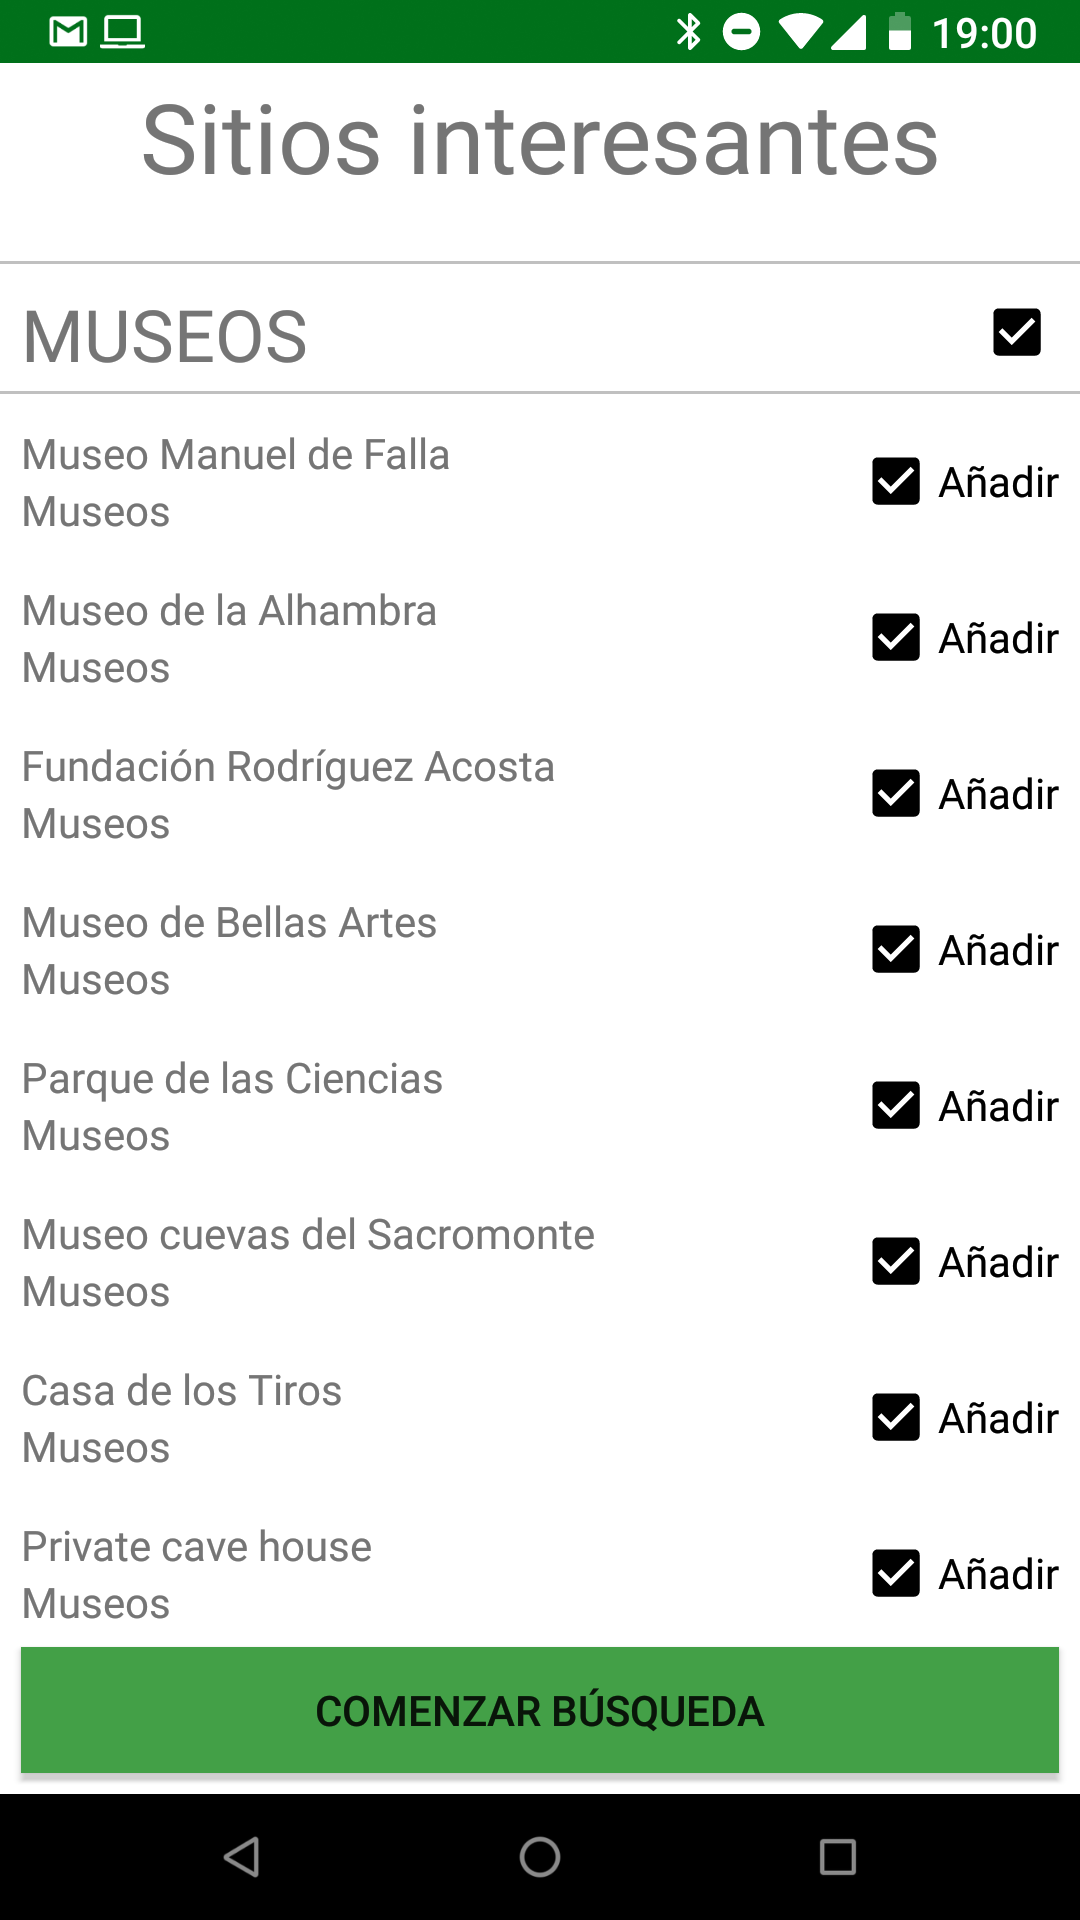
\includegraphics[width=50mm]{imagenes/seleccion_museos}
	\caption{Selección de todos los museos disponibles dentro de la aplicación.}
	\label{fig:selec_museos}
\end{figure}
\begin{figure}[H]
	\centering
	\subfigure{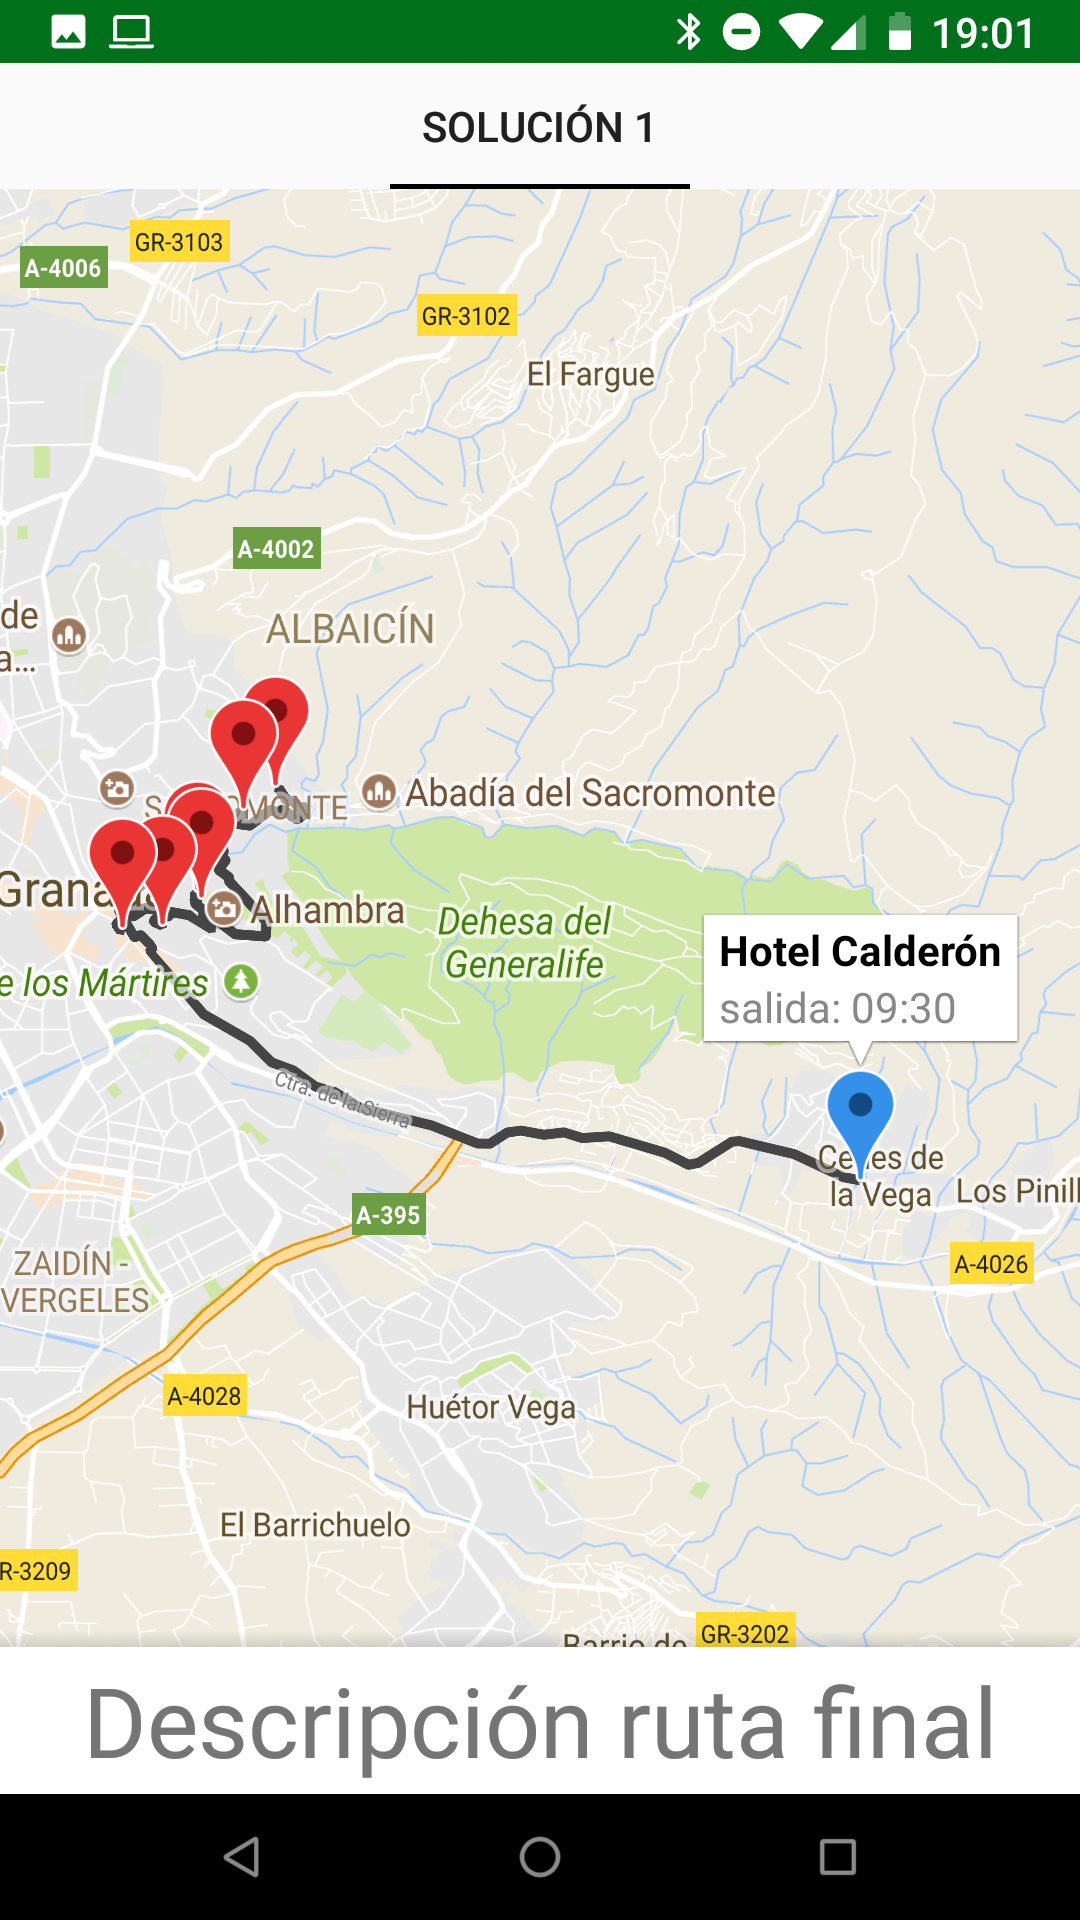
\includegraphics[width=40mm]{imagenes/salida_1}}
	\subfigure{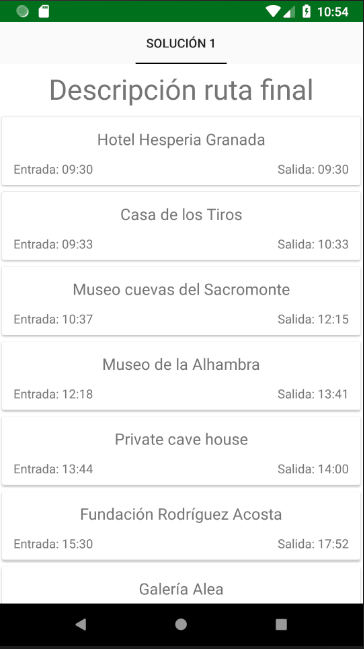
\includegraphics[width=40mm]{imagenes/descripcion_ruta}}
	\caption{Ruta obtenida para el alojamiento seleccionado y todos los museos seleccionados.}
	\label{fig:salida}
\end{figure}

\section[Caso 2]{Ruta sobre un conjunto específico de puntos de interés}
Si se da el caso de que el usuario quiera visitar unos puntos de interés también puede hacerlo; para este ejemplo se van a seleccionar el mirador de San Nicolás, la Hermita de San Miguel Alto, la Catedral de Granada y el Parque de las Ciencias. Para seleccionar dichos puntos, el usuario debe buscarlos dentro de la lista; al igual que se muestran en las figuras \ref{fig:seleccion_multiple}.\newline

Tras esto, el usuario deberá iniciar la búsqueda para pulsar el botón \enquote{Comenzar búsqueda}. Tras esto, se mostrará el resultado, dicho resultado es el que se puede ver en las figuras \ref{fig:salida_2}.Al ser pocos puntos de interés, la solución selecciona todos los puntos de interés.\newline

\begin{figure}[H]
	\centering
	\subfigure{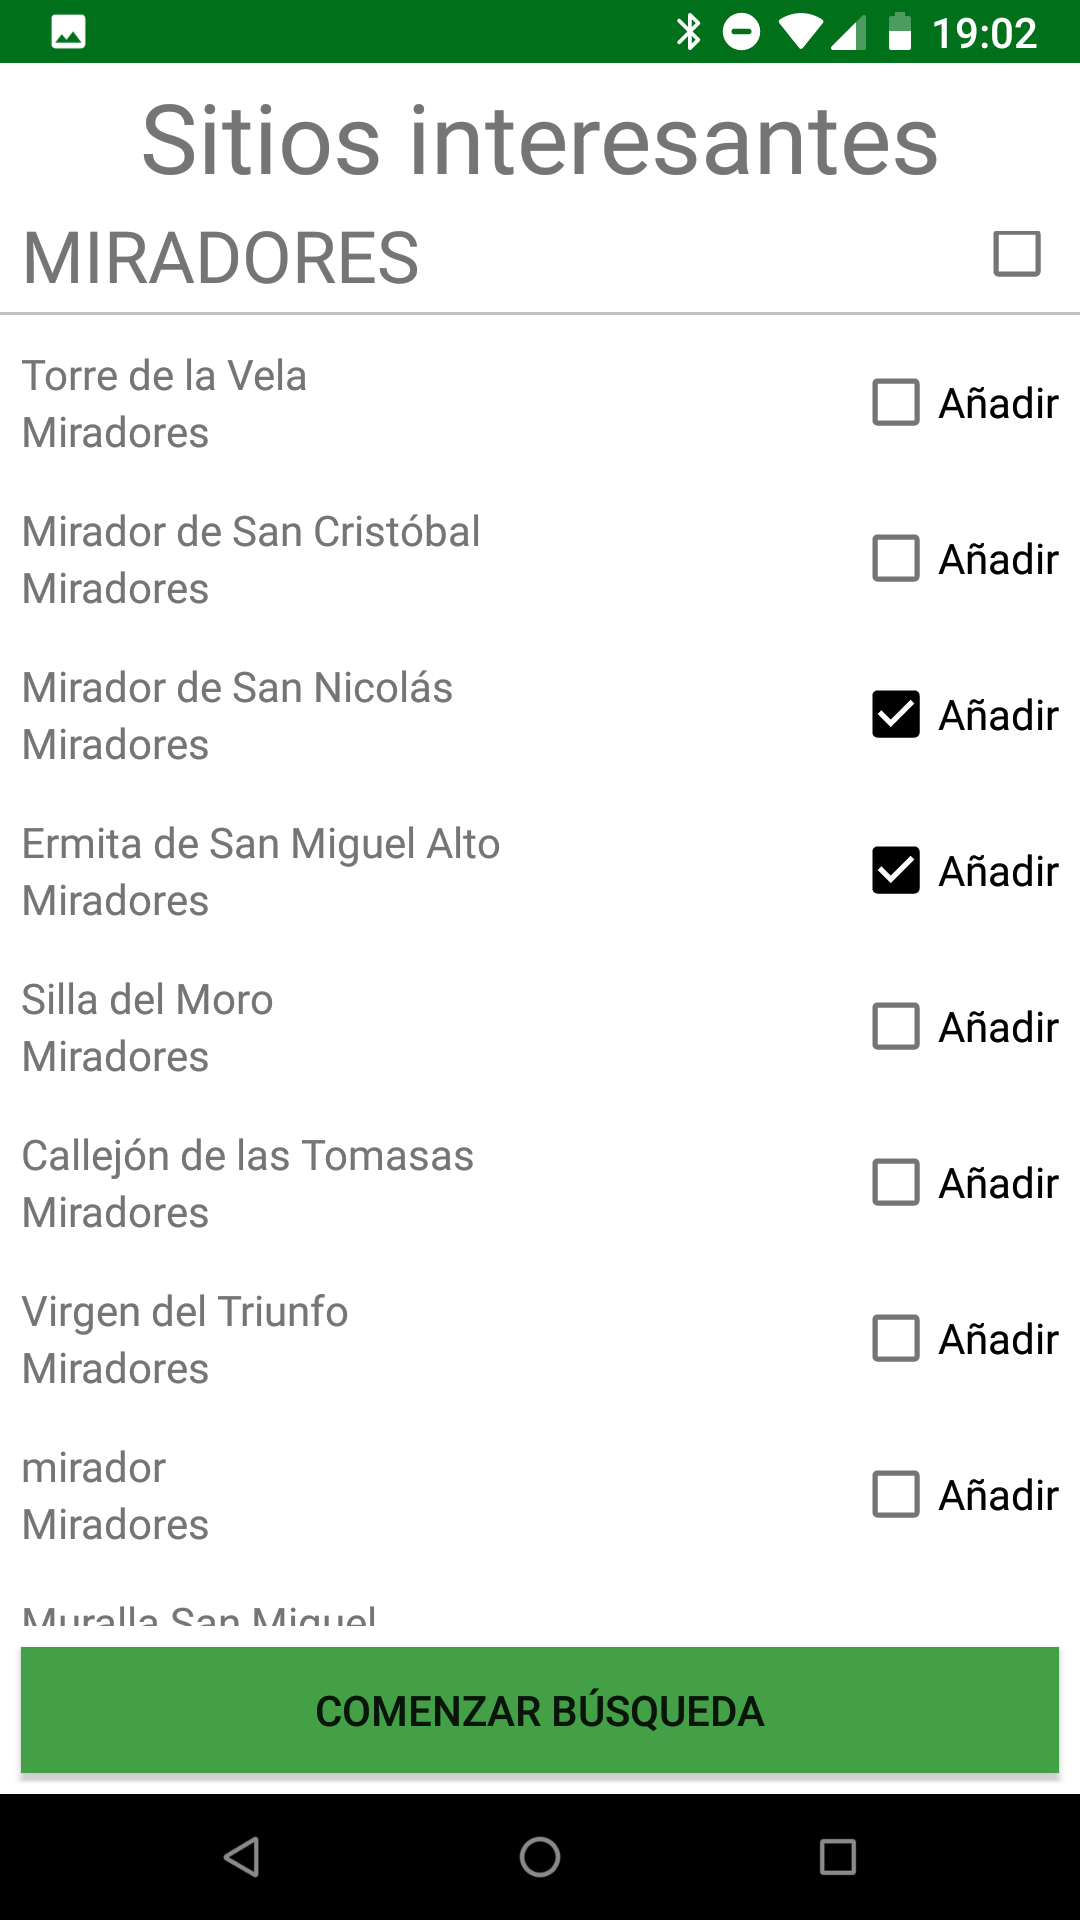
\includegraphics[width=45mm]{imagenes/seleccion_miradores}}
	\subfigure{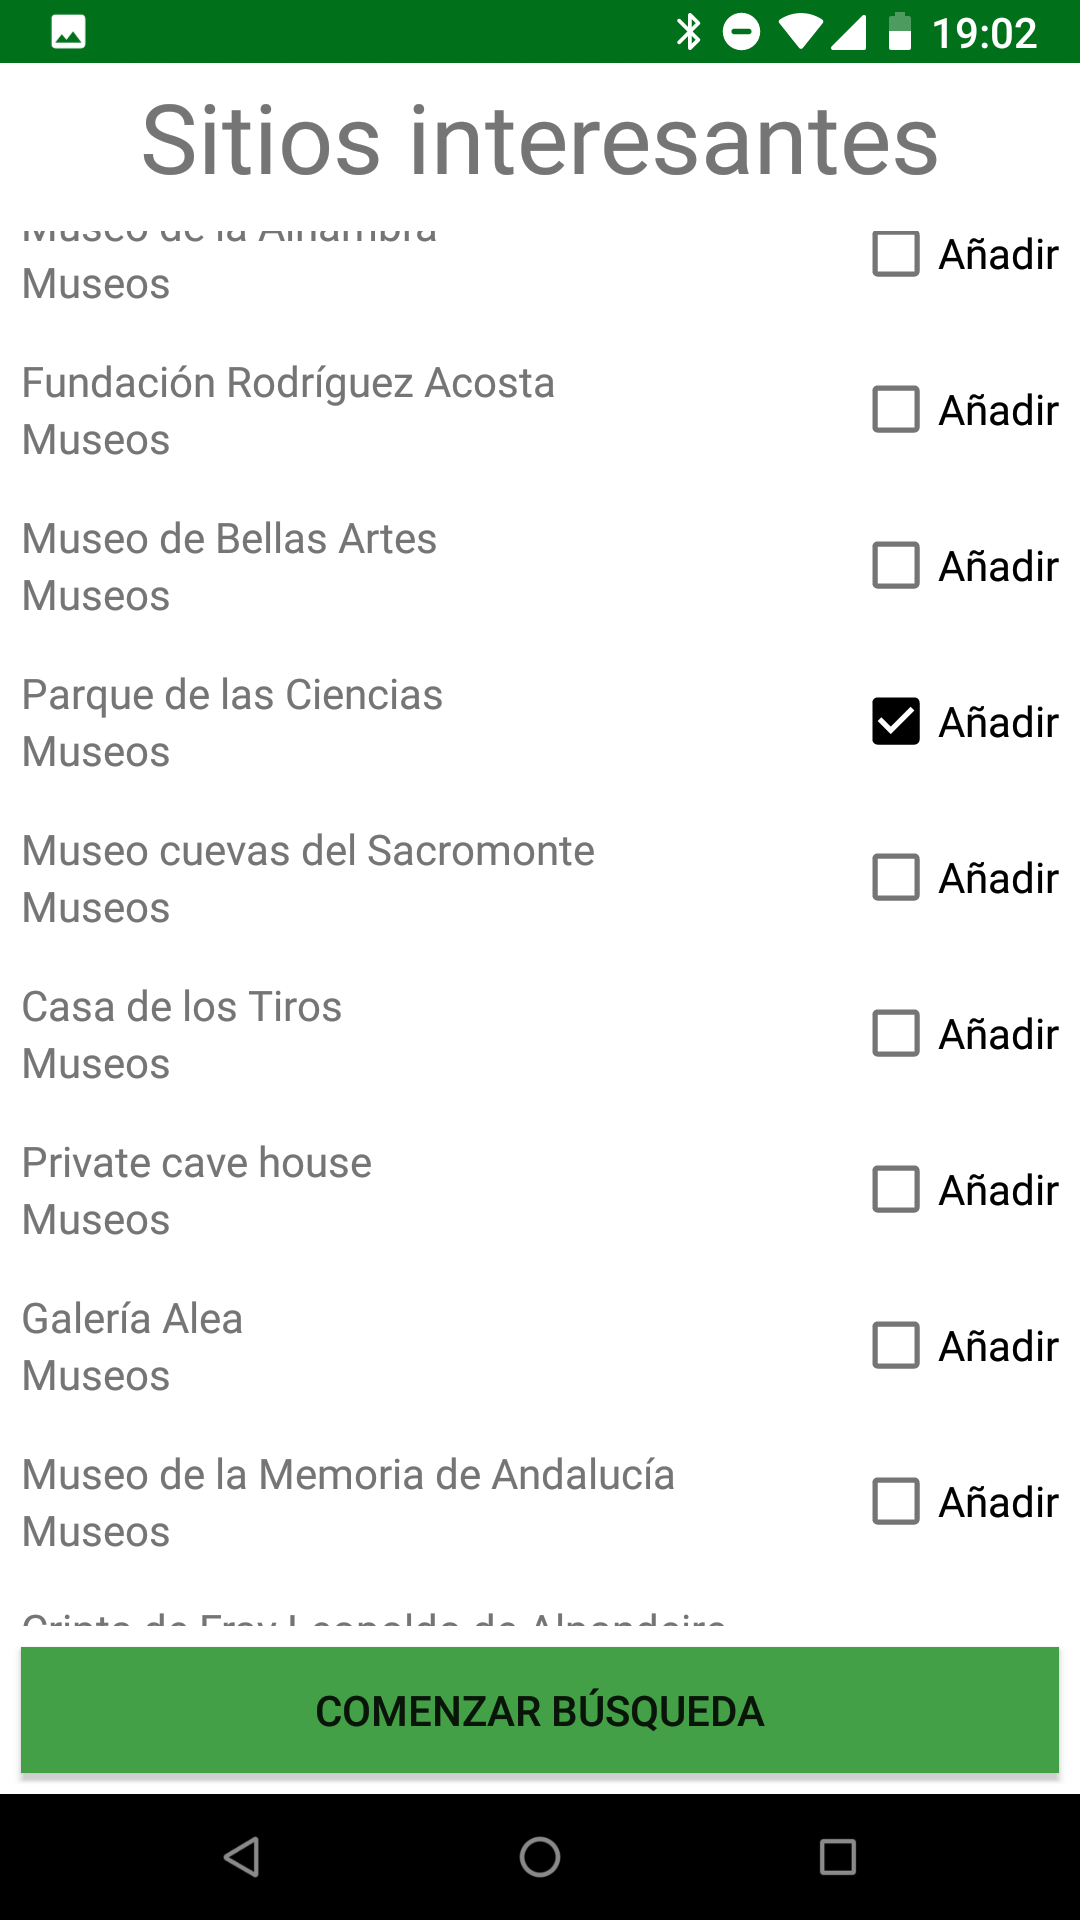
\includegraphics[width=45mm]{imagenes/seleccion_parque}}
	\subfigure{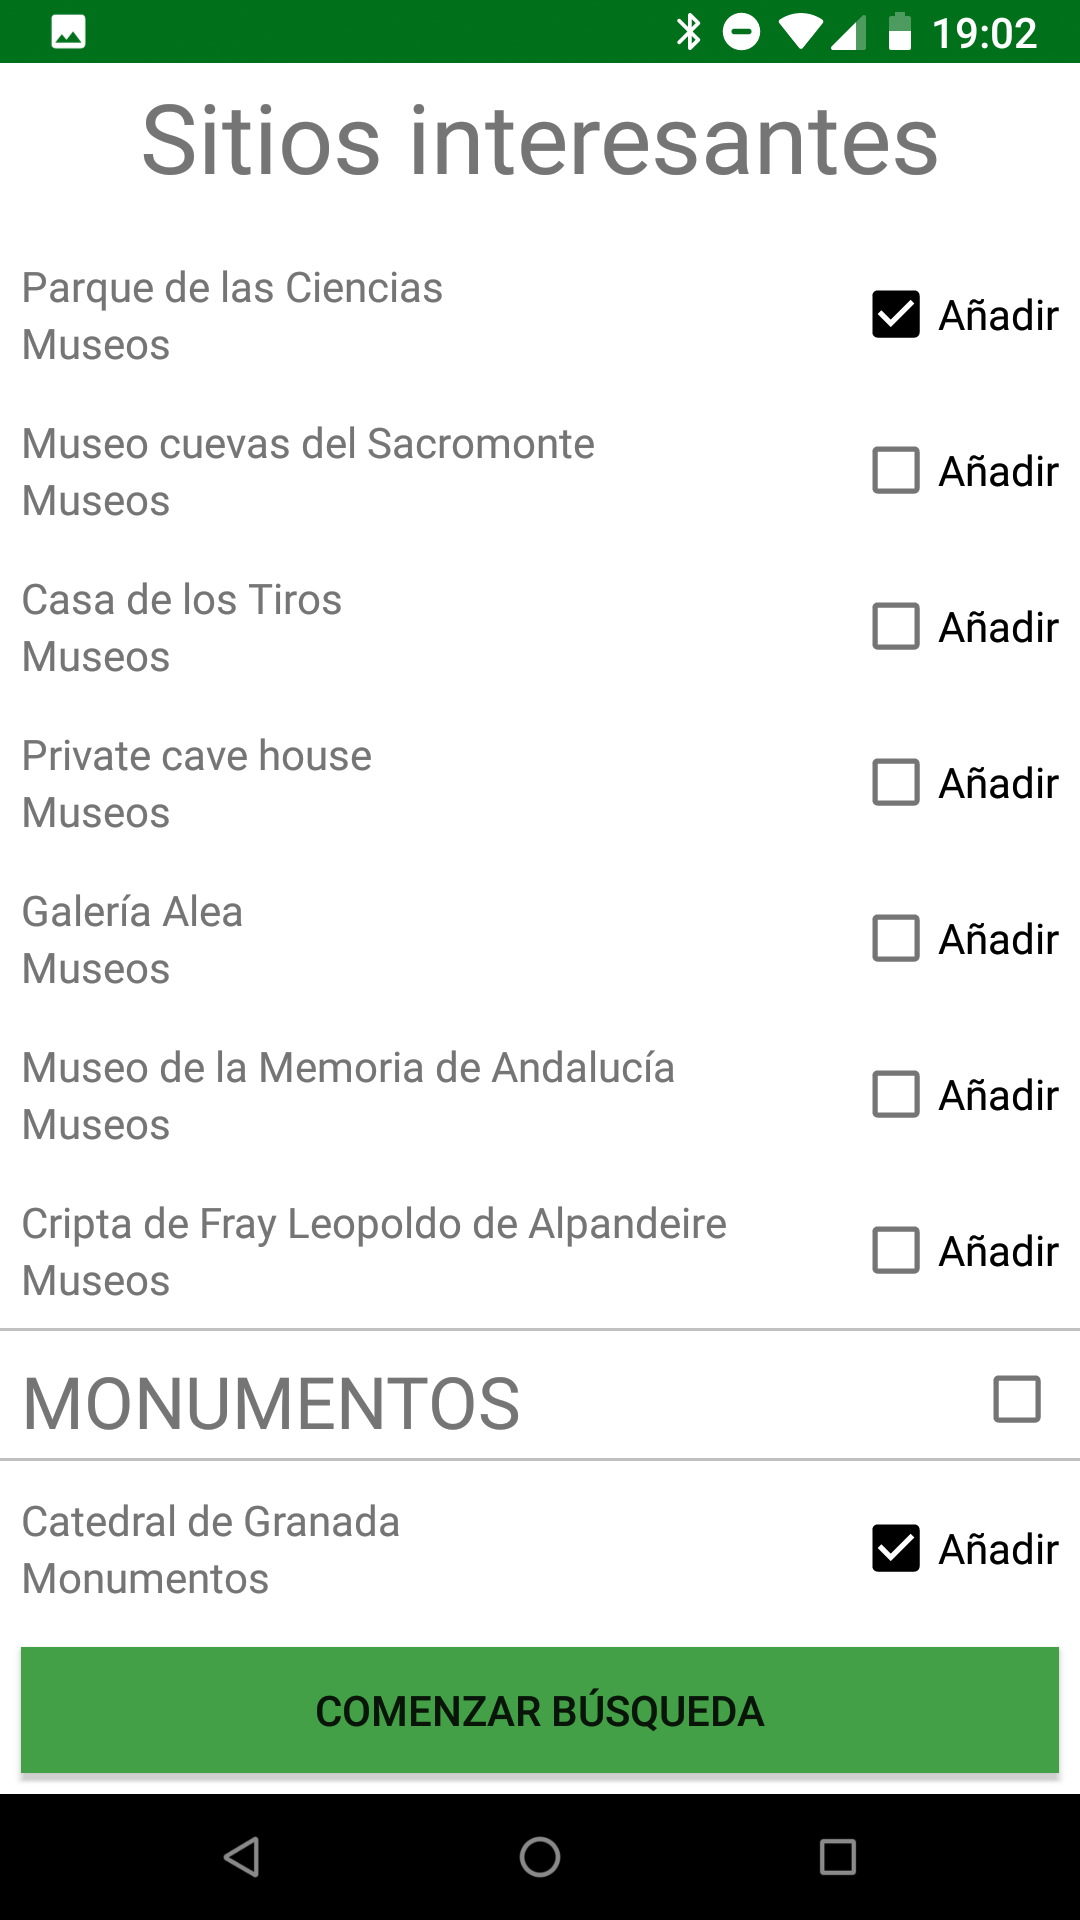
\includegraphics[width=45mm]{imagenes/seleccion_catedral}}
	\caption{Selección de un subconjunto específico de punto de interés.}
	\label{fig:seleccion_multiple}
\end{figure}
\begin{figure}[H]
	\centering
	\subfigure{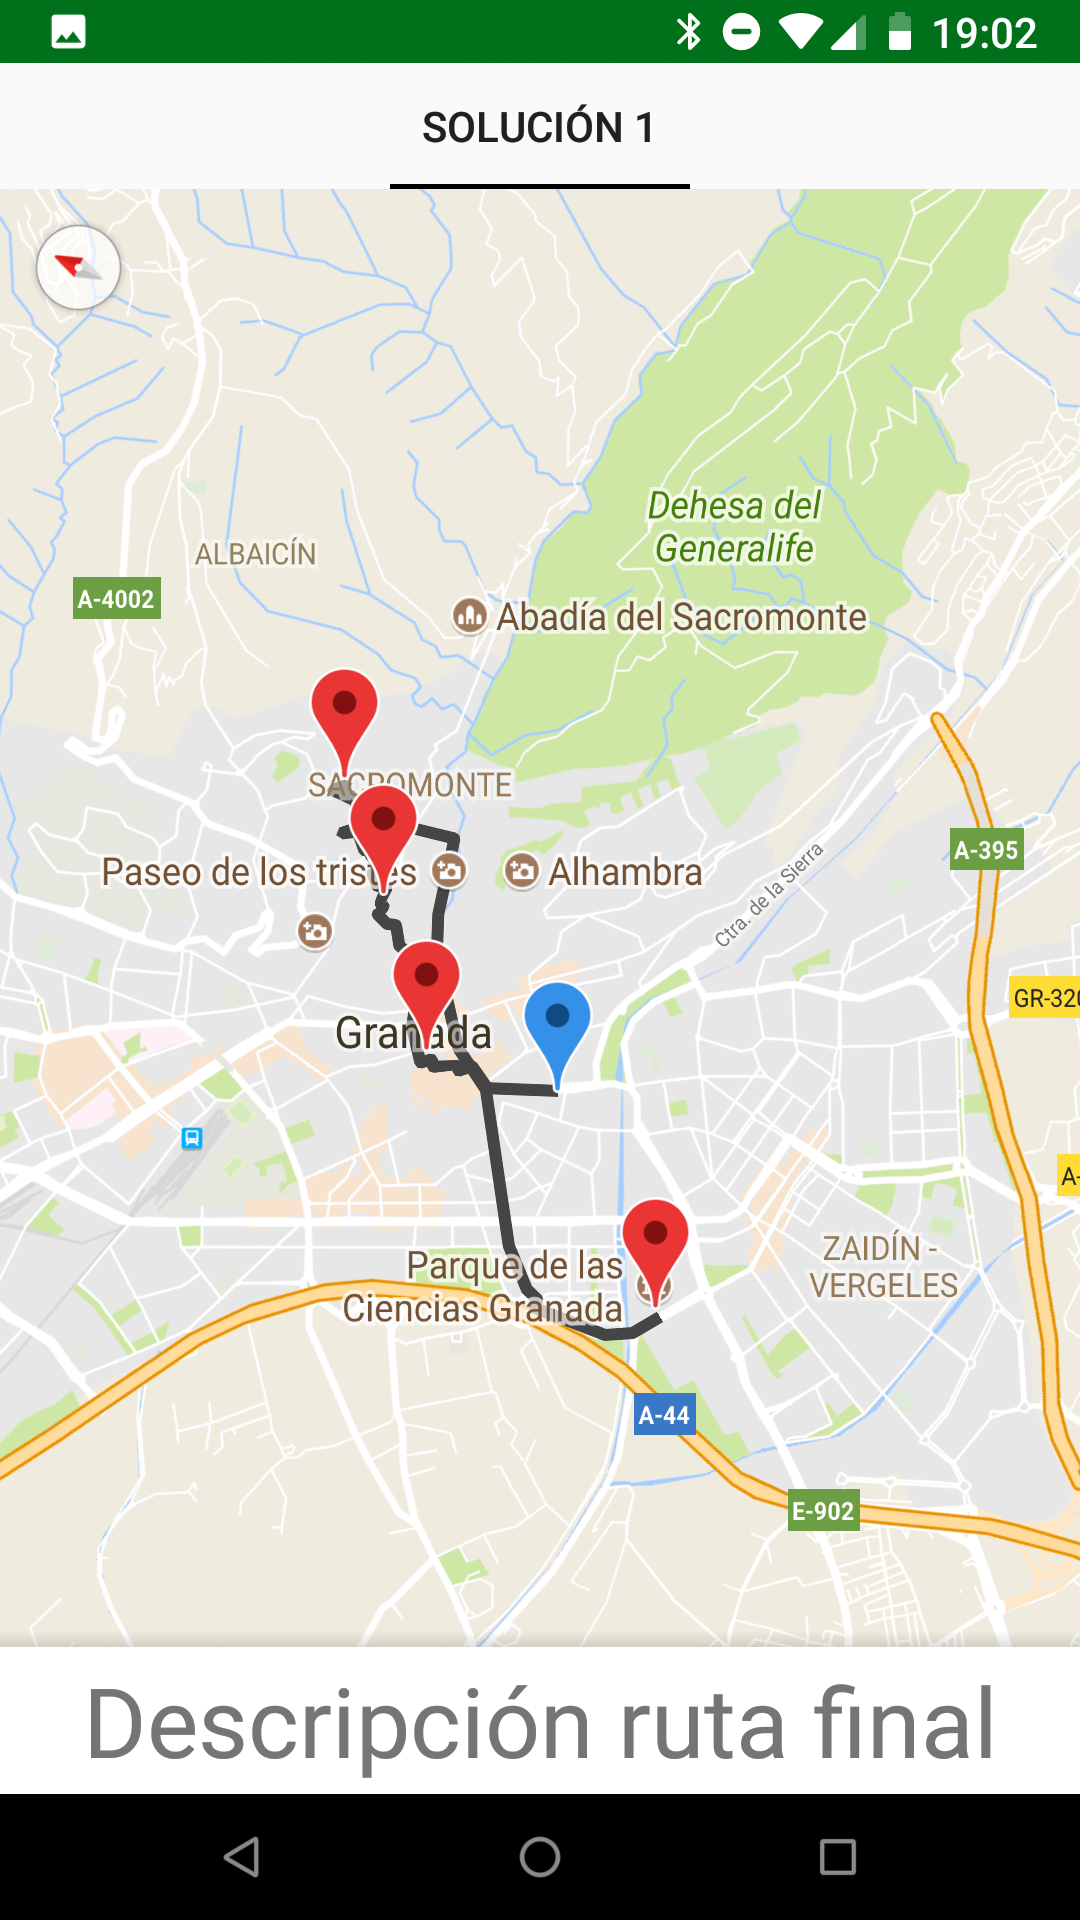
\includegraphics[width=40mm]{imagenes/salida_2}}
	\subfigure{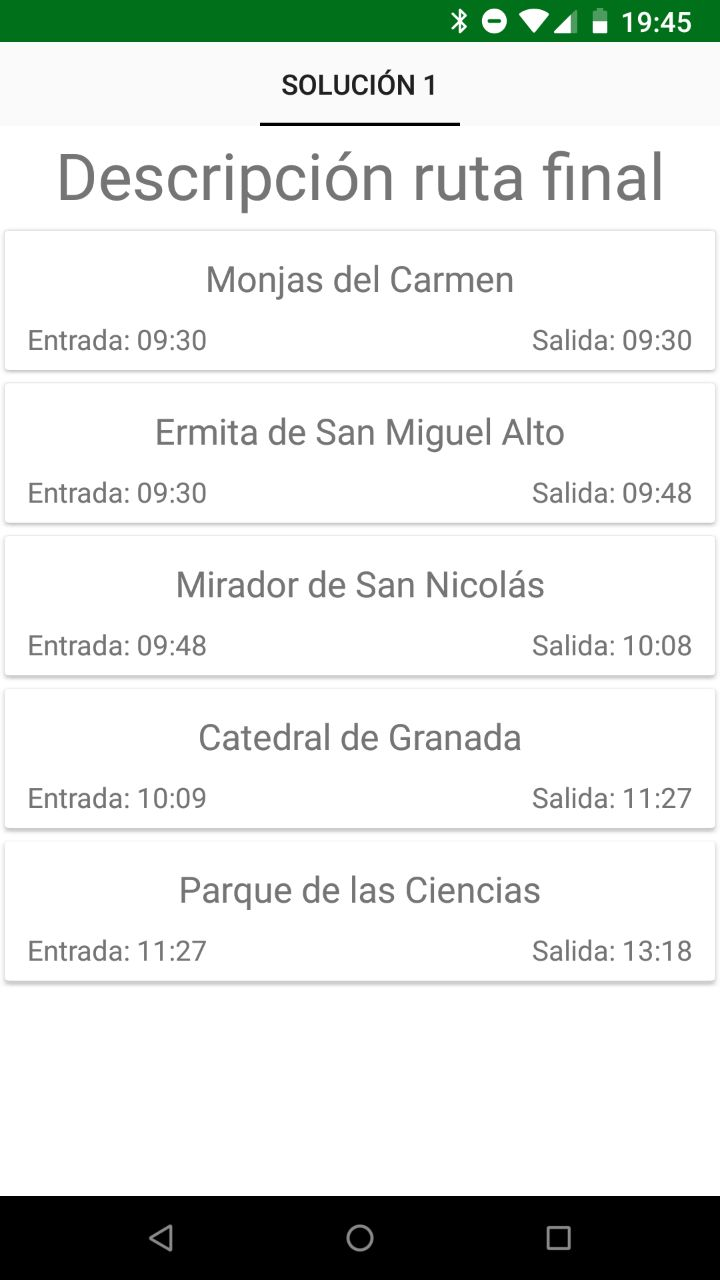
\includegraphics[width=40mm]{imagenes/descripcion_2}}
	\caption{Ruta calculada para el conjunto de puntos de interés.}
	\label{fig:salida_2}
\end{figure}
%
%\chapter{Conclusiones}
%
%%\chapter{Conclusiones y Trabajos Futuros}
%
%
%%\nocite{*}
%\bibliography{bibliografia/bibliografia}\addcontentsline{toc}{chapter}{Bibliografía}
%\bibliographystyle{miunsrturl}
%
%\appendix
%\input{apendices/manual_usuario/manual_usuario}
%%\input{apendices/paper/paper}
%\huge \textbf{Glosario}
\normalsize
\begin{itemize}
	\item \textbf{Activity:} es una componente de la aplicación que contiene una pantalla con la que un usuario puede interactuar. Cada actividad tiene una pantalla asociada a una interfaz de usuario. Normalmente la pantalla suele ocupar toda la pantalla.
	\item \textbf{Fragment:} representa un comportamiento o parte de la interfaz de usuario de una Activity. Dentro de una Activity se pueden combinar varios Fragments. Al igual que una Activity, tiene un ciclo de vida propio y recibe sus propios eventos de entrada. Podría definirse como una \enquote{subactividad}.
	\item \textbf{View:} representa el bloque básico para representar cualquier elemento básico de la interfaz de usuario en Android.
	\item \textbf{ViewGroup:} es un tipo especial de View que puede contener Views a su vez. Este tipo de View es utilizada como base de un Layout y otro contenedores complejos dentro de Android.
	\item \textbf{Layout:} define la estructura para el diseño de una interfaz de usuario, como la UI de una actividad o un widget de una aplicación.
\end{itemize}

% \addcontentsline{toc}{chapter}{Glosario}
% \printglossary
\chapter*{}
\thispagestyle{empty}

\end{document}
